% !TeX root = main_submission.tex

\documentclass[superscriptaddress,
               floatfix,
               longbibliography, 
               showkeys,apl]{revtex4-2}  
  
%\bibliographystyle{apsrevtitle}

\usepackage{graphicx} 
\usepackage{bm}	
\usepackage{color}                     
\usepackage{xcolor}
\usepackage{epsfig}
\usepackage{amsmath} 
\usepackage{amssymb} 
\usepackage{longtable} 
\usepackage{float}
\usepackage{mathtools}
\usepackage{dsfont}
\usepackage{xparse}
\usepackage{hyperref}
\usepackage{times}
\usepackage[normalem]{ulem}
\usepackage{sidecap}
\usepackage{appendix} 
\sidecaptionvpos{figure}{t}
\usepackage{comment}
\usepackage{physics}
\usepackage{float}
\usepackage{xfrac}
\newtheorem{theorem}{Theorem}
\usepackage{svg}
\usepackage{multirow}
\usepackage{algpseudocode}
\usepackage{tikz,lipsum,lmodern}
\usepackage[most]{tcolorbox}
\usepackage{tikz}

%% Text flags
\definecolor{darkgreen}{rgb}{0.0, 0.5, 0.0}
\newcommand{\wip}[2]{\textcolor{darkgreen}{[#1] #2}}

%\newcommand{\eg}{e.g.}
%\newcommand{\ie}{i.e.}

%PQC tasks
\newcommand{\ansatz}{\mathcal{U}} % Ansatz
\newcommand{\pqc}{\ansatz(\params)} % PQC

\newcommand{\objective}{C} % cost operator
\newcommand{\objectiveparams}{\objective(\params)} % cost operator

\newcommand{\costfunction}{\mathcal{C}} % PQC
\newcommand{\costfunctionstate}{\costfunction(\psi)} % PQC
\newcommand{\costoperator}{\mathcal{O}} % cost operator

\newcommand{\taskidx}{\tau} % cost operator
\newcommand{\taskidxtest}{\tau^{\prime}} % cost operator
\newcommand{\stateinit}{|\psi_0 \rangle} % cost operator
\newcommand{\statefinal}{|\psi(\params) \rangle}
\newcommand{\state}{|\psi \rangle}

\newcommand{\proj}[1]{|#1\rangle \langle #1|}


\newcommand{\be}{\begin{equation}}
\newcommand{\ee}{\end{equation}}
\newcommand{\bd}{\begin{displaymath}}
\newcommand{\ed}{\end{displaymath}}
\newcommand{\BE}{\begin{eqnarray}}
\newcommand{\EE}{\end{eqnarray}}
\newcommand{\vsp}{\vspace*{3mm}}
\newcommand{\pprime}{{\prime\prime}}
\newcommand{\R}{{\rm I\!R}}
\newcommand{\smallo}{{o}}
\newcommand{\plus}{{\!+\!}}
\newcommand{\minus}{{\!-\!}}
\newcommand{\sgn}{{\rm sgn}}
\newcommand{\erfc}{{\rm erfc}}
\newcommand{\id}{{\rm 1\!\!I}}
\newcommand{\ba}{\ensuremath{\mathbf{a}}}
\newcommand{\bb}{\ensuremath{\mathbf{b}}}
\newcommand{\bc}{\ensuremath{\mathbf{c}}}
\newcommand{\bh}{\ensuremath{\mathbf{h}}}
\newcommand{\bk}{\ensuremath{\mathbf{k}}}
\newcommand{\bq}{\ensuremath{\mathbf{q}}}
\newcommand{\bs}{\ensuremath{\mathbf{s}}}
\newcommand{\bu}{\ensuremath{\mathbf{u}}}
\newcommand{\bv}{\ensuremath{\mathbf{v}}}
\newcommand{\bw}{\ensuremath{\mathbf{w}}}
\newcommand{\bx}{\ensuremath{\mathbf{x}}}
\newcommand{\by}{\ensuremath{\mathbf{y}}}
\newcommand{\bz}{\ensuremath{\mathbf{z}}}
\newcommand{\bn}{\ensuremath{\mathbf{n}}}
\newcommand{\bolde}{\ensuremath{\mathbf{e}}}
\newcommand{\bee}{\ensuremath{\mathbf{e}}}
\newcommand{\boldeff}{\ensuremath{\mathbf{f}}}
\newcommand{\bA}{\ensuremath{\mathbf{A}}}
\newcommand{\bB}{\ensuremath{\mathbf{B}}}
\newcommand{\bC}{\ensuremath{\mathbf{C}}}
\newcommand{\bD}{\ensuremath{\mathbf{D}}}
\newcommand{\bF}{\ensuremath{\mathbf{F}}}
\newcommand{\bG}{\ensuremath{\mathbf{G}}}
\newcommand{\bGz}{\ensuremath{\mathbf{G_0}}}
\newcommand{\bRone}{\ensuremath{\mathbf{R_1}}}
\newcommand{\bJ}{\ensuremath{\mathbf{J}}}
\newcommand{\bK}{\ensuremath{\mathbf{K}}}
\newcommand{\bR}{\ensuremath{\mathbf{R}}}
\newcommand{\bT}{\ensuremath{\mathbf{T}}}
\newcommand{\bW}{\ensuremath{\mathbf{W}}}
\newcommand{\bM}{\ensuremath{\mathbf{M}}}
\newcommand{\bp}{\ensuremath{\mathbf{p}}}
\newcommand{\bCx}{\ensuremath{\mathbf{C_1}}}
\newcommand{\bCy}{\ensuremath{\mathbf{C_2}}}
\newcommand{\bGx}{\ensuremath{\mathbf{G_1}}}
\newcommand{\bGy}{\ensuremath{\mathbf{G_2}}}
\newcommand{\beff}{\ensuremath{\mathbf{f}}}
\newcommand{\hq}{\hat{q}}
\newcommand{\hw}{\hat{w}}
\newcommand{\hx}{\hat{x}}
\newcommand{\hy}{\hat{y}}
\newcommand{\hA}{\hat{A}}
\newcommand{\hC}{\hat{C}}
\newcommand{\hG}{\hat{G}}
\newcommand{\hK}{\hat{K}}
\newcommand{\hL}{\hat{L}}
\newcommand{\D}{{\cal{D}}}
\newcommand{\hbq}{\hat{\mbox{\boldmath{q}}}}
\newcommand{\qbo}{{\mbox{\boldmath{q}}}}
\newcommand{\hbx}{\hat{\mbox{\boldmath{x}}}}
\newcommand{\hbw}{\hat{\mbox{\boldmath{w}}}}
\newcommand{\hOmega}{\hat{\mbox{$\Omega$}}}
\newcommand{\bchi}{{\mbox{\boldmath{$\chi$}}}}
\newcommand{\boldeta}{{\mbox{\boldmath{$\eta$}}}}
\newcommand{\boldomega}{{\mbox{\boldmath{$\omega$}}}}
\newcommand{\boldpsi}{{\mbox{\boldmath{$\psi$}}}}
\newcommand{\boldphi}{{\mbox{\boldmath{$\varphi$}}}}
\newcommand{\bEta}{{\mbox{\boldmath{$\eta$}}}}
\newcommand{\bzeta}{{\mbox{\boldmath{$\zeta$}}}}
\newcommand{\boldOmega}{{\mbox{\boldmath{$\Omega$}}}}
\newcommand{\bxi}{\bm{\xi}}
\newcommand{\olx}{\overline{\mathbf{x}}}
\newcommand{\olxone}{\overline{x}_1}
\newcommand{\olxtwo}{\overline{x}_2}
\newcommand{\olxonedot}{\dot{\overline{x}}_1}
\newcommand{\olxtwodot}{\dot{\overline{x}}_2}
\newcommand{\bnull}{{\mbox{\boldmath{$0$}}}}
\newcommand{\rate}{\tilde{\eta}}
\newcommand{\double}{{\prime\prime}}
\newcommand{\tp}{t^\prime}
\newcommand{\td}{t^{\prime\prime}}
\newcommand{\wt}{\widetilde}
\newcommand{\avg}[1]{\left\langle{#1}\right\rangle}
\newcommand{\davg}[1]{\left\langle\left\langle{#1}\right\rangle\right\rangle}
\newcommand{\fE}{\mathbb{E}}
\newcommand{\ds}{\mathcal{D}\,\mathbf{S}}
\newcommand{\mcD}{\mathcal{D}}
\newcommand{\mcM}{\mathcal{M}}

\newcommand{\Jferro}{J_{\mathrm{F}}}


\newcommand{\Ham}[1]{H_{\mathrm{#1}}}
\newcommand{\Hnumfault}{\Ham{numfaults}}
\newcommand{\Hgate}{\Ham{gate}}
\newcommand{\Hfaultset}{\Ham{faultset}}
\newcommand{\Hconsist}{\Ham{consist}}
\newcommand{\Hmultfault}{\Ham{multfault}}
\newcommand{\weight}[1]{\lambda_{\mathrm{#1}}}
\newcommand{\faultweight}{\weight{faultset}}
\newcommand{\multfaultweight}{\weight{multfault}}
\newcommand{\gateweight}{\weight{gate}}
\newcommand{\OR}{\textsc{OR}}
\newcommand{\AND}{\textsc{AND}}
\newcommand{\XOR}{\textsc{XOR}}
\newcommand{\EQ}{\textsc{EQ}}
\newcommand{\BUFFER}{\textsc{BUFFER}}
\newcommand{\NOR}{\textsc{NOR}}
\newcommand{\NOT}{\textsc{NOT}}
\newcommand{\NAND}{\textsc{NAND}}

\renewcommand{\labelenumi}{(\roman{enumi})}
\newcommand{\expectedval}[1]{{\mathbb E}\left[ #1 \right]}
\newcommand{\probability}[1]{{\mathbb P}\left[ #1 \right]}


\DeclareMathOperator{\sign}{sign}
\DeclareMathOperator*{\argmin}{arg\,min}

\providecommand{\abs}[1]{\lvert#1\rvert}

\def\c#1{\textcolor{blue}{#1}}
\def\cc#1{\textcolor{red}{#1}}
\def\ccc#1{\textcolor{green}{#1}}

\newcommand{\fs}[1]{\textcolor{blue}{#1}}
\def\hs#1{\textcolor{magenta}{[#1]}}
\newcommand{\ws}[1]{\textcolor{orange}{#1}}
\newcommand{\pjl}[1]{\textcolor{darkgreen}{#1}}
\def\aak#1{\textcolor{orange}{[#1]}}
\def\apo#1{\textcolor{cyan}{#1}}
\def\apoNote#1{\textcolor{cyan}{\textbf{ [#1]} }}

\def\mm#1{\textcolor{green!10!orange!90!}{#1}}


%\NewDocumentCommand{\ceil}{s O{} m}{
%  \IfBooleanTF{#1} 
%    {\left\lceil#3\right\rceil} 
%    {#2\lceil#3#2\rceil} 
%}

\hyphenation{OptDigits}

\begin{document}


\title{Sparse Block-Encodings for Linear Combinations of Ladder Operators}


\date{\today} 

% \ws{You can make comments}
% \gus{using your shortcut}
% \ks{and it'll put}
% \ar{your comments}
% \pjl{in your own color :D}

\begin{abstract}
\label{abstract}

In this work, we detail the construction of block-encodings for observables described as a linear combination of products of ladder operators acting on fermionic, antifermionic, and bosonic modes.
We refer to this constuction as LOBE (Ladder Operator Block-Encoding) and show how it can be used to simulate Hamiltonians involving interactions between these different types of particles.
Our work builds off of similar sparse block-encoding constructions for fermionic system, but generalizes them to include bosonic ladder operators.
Additionally, we establish a clear connection between these sparse block-encodings and LCU (Linear Combination of Unitaries) block-encodings.
This connection allows for implementations of these block-encodings that significantly reduce the rescaling factor of the block-encoding without significantly affecting the quantum resources required to implement the block-encoding.
Constructing efficient block-encodings that allow for interactions between fermions, antifermions, and bosons, paves the way for the simulation of systems that are not purely fermionic which is vital for the simulation of many models that arise in high-energy physics.

\end{abstract} 

\maketitle

\section{Introduction}
\label{sec:intro}

The simulation of many-body quantum systems is a promising potential application for quantum computers \cite{feynman2018simulating}.
Accessing the information of non-unitary operators - such as the Hamiltonian - within a quantum algorithm, which is comprised solely of unitary operations, is a necessary subroutine for performing such simulations.
This task has been pursued through various means, resulting in methods such as Trotterization \cite{suzuki1976generalized,hatano2005finding,lie1893theorie,trotter1959product,childs2021theory} and Block-Encoding \cite{lin2022lecture, poulin2018quantum, low2019hamiltonian}.

Block-Encoding describes a general strategy for encoding a non-unitary operator within a chosen subspace (block) of a larger unitary operator.
Two general frameworks for constructing block-encodings of different operators - sparse block-encodings \cite{berry2009black, childs2009universal, lin2022lecture} and Linear Combinations of Unitaries (LCU) \cite{childs2012hamiltonian} - have allowed for the exploration of explicitly compiled block-encodings of several systems.

Understanding the spacetime quantum resources - the number of qubits (space), the number of operations (time), and the rescaling factor (overhead) - required for quantum simulation algorithms is important for understanding the feasability of simulating different systems.
These quantum resource estimates are crucial as they allow us to gauge the practical usefulness of quantum computers, particularly those that have experimentally demonstrated quantum error correction \cite{bluvstein2024logical, acharya2024quantum}.

Many previous works have investigated the quantum simulation for purely fermionic systems, with a particular emphasis on the simulation of molecules in quantum chemistry \cite{aspuru2005simulated, peruzzo2014variational, babbush2014adiabatic, o2016scalable, babbush2018encoding, google2020hartree, lee2021even, kivlichan2020improved, campbell2021early}.
Another interesting set of quantum systems to simulate are those that are derived from quantum field theories \cite{Peskin:1995ev, jordan2012quantum} \ws{@Gus, pls add citation for all models (quartic, static, phi, yukawa)}, which have applications in areas such as high-energy physics \cite{bauer2023quantum}.
These systems often include interactions between fermions, antifermions, and bosons and several works have produced quantum resource estimates for simulating such systems \cite{camps2024explicit, liu2024efficient, rhodes2024exponential}.

In this work, we provide a novel framework for constructing block-encodings of second-quantized operators, which we refer to as Ladder-Operator Block-Encoding (LOBE).
This framework directly block-encodes operators comprised of creation and annihilation operators and does not require the use of operator transformations that expand fermionic \cite{jordan1928paulische, bravyi2002fermionic, seeley2012bravyi} and bosonic \cite{somma2005quantum} \ws{add standard binary citations} ladder operators in the Pauli operator basis.

We give numerical quantum resource estimates for implementing block-encodings of several classes of operators and several Hamiltonians that arise in quantum field theories.
This includes purely fermionic systems, purely bosonic systems, and systems which include fermions, antifermions, and bosons. 
We analyze the numerical spacetime quantum resources for LOBE - in comparison to techniques which require mapping ladder operators onto the Pauli basis - and find that LOBE results in constructions with better asymptotic scaling and lower numerical quantum resources for many of the systems examined.

This work is organized as follows.
In Section \ref{sec:theory}, we review the defined action of ladder operators on quantum states.
In Section \ref{sec:block-encoding}, we review block-encodings and discuss frameworks for constructing block-encodings of different operators.
In Section \ref{sec:ladder-op-oracles}, we describe the LOBE framework, show compiled block-encodings for several classes of second-quantized operators, and give analytical spacetime costs of the associated constructions.
In Section \ref{sec:results}, we provide numerical quantum resource estimates for block-encodings of various classes of operators and Hamiltonians.
In Section \ref{sec:conclusions}, we summarize the results presented in this work and discuss future directions.
Additionally, a glossary that defines the terminology and variables used throughout this work is given in Appendix \ref{sec:glossary}.

\section{Theory}

Give background of ladder operators and constructions of realistic Hamiltonians/Observables from ladder operators

\subsection{Encoding}
\label{subsec:encoding}

Here we'll discuss how we encode the physical states we are interested in terms of qubits/registers.

\ws{Question: do we want to also cost-out the unary encoding or just the "compact" encoding that we've been primarily working with?}

\subsection{Ladder Operators}
\label{subsec:operators}

\ws{@Gus, you probably have much better language to define all of this stuff. I just needed to write something down so I could reference it in the circuit construction. Don't hesitate to scrap anything in here.}


\subsubsection{Feromons and Antiferomons}

Define action of fermionic ladder operators.

Fermions (and antifermions) obey the Pauli-exclusion principle \ws{citation} and therefore the occupation of a (anti)fermionic mode can only be occupied ($\ket{1}$) or unoccupied ($\ket{0}$).
Fermionic (and antifermionic) ladder operators only act non-trivially on the qubits encoding the mode that the ladder operator acts on and we define their action as follows.

The fermionic creation operator is given by:
\begin{equation}
    b_i^\dagger \ket{n_{b_i}} = 
    \begin{cases} 
        (-1)^{\sum_{j < i} b_j} \ket{1}  & when \ket{n_{b_i}} is \ket{0} \\
        0 & when \ket{n_{b_i}} is \ket{1}
    \end{cases}
\end{equation}
where $b_i$ denotes a fermionic ladder operator on the $i^{th}$ mode, the $^\dagger$ indicates a creation operator, and $\ket{n_{b_i}}$ is the occupation of the $i^{th}$ fermionic mode.
An antifermionic creation operator is defined as above with the symbol $d$ to denote that the operator acts on antifermions.

For a fermionic creation operator, if the mode being acted upon is unoccupied, then the creation operator "creates" a fermion in that mode and applies a phase determined by the parity of the occupation of the previous modes.
Therefore the ordering of the modes in the encoding has an implication on the action of the operator that must be accounted for.
Since fermionic modes can only be either occupied or unoccupied, then if the mode is already occupied the operator zeroes the amplitude of the quantum state, thereby "destoying" that portion of the quantum state. 

The fermionic annihilation operator is given by:
\begin{equation}
    b_i \ket{n_{b_i}} = 
    \begin{cases} 
        (-1)^{\sum_{j < i} b_j} \ket{0}  & when \ket{n_{b_i}} = \ket{1} \\
        0 & when \ket{n_{b_i}} = \ket{0}
    \end{cases}
\end{equation}
and the antifermionic annihilation operator is likewise defined for $d$ instead of $b$.

The action of the annihilation operators is similar (and opposite) to the creation operators.
If the mode is already occupied, then the annihilation operator "annihilates" the fermion at that mode by setting the occupation to zero and applies a phase based on the parity of the occupation of the preceeding modes.
If the mode is unoccupied before the operator is applied, then the annihilation operator zeroes the amplitude.

\subsubsection{Bosos}

\begin{equation}
    a_i^\dagger \ket{n_{a_i}} = 
    \begin{cases} 
        \sqrt{n_{a_i} + 1} \ket{n_{a_i} + 1}  & when \ket{n_{a_i}} \neq \ket{\Omega} \\
        0 & when \ket{n_{a_i}} = \ket{\Omega}
    \end{cases}
\end{equation}
where $a_i$ denotes a bosonic ladder operator on the $i^{th}$ mode, the $^\dagger$ indicates a creation operator, $\ket{n_{a_i}}$ is the occupation of the $i^{th}$ bosonic mode, and $\Omega$ is the maximum allowable bosonic occupation.

\begin{equation}
    a_i \ket{n_{a_i}} = 
    \begin{cases} 
        \sqrt{n_{a_i}} \ket{n_{a_i} - 1}  & when \ket{n_{a_i}} \neq \ket{0} \\
        0 & when \ket{n_{a_i}} = \ket{0}
    \end{cases}
\end{equation}

\subsubsection{Commutation Rules}
\label{subsec:commutation}


\subsection{Observables}
\label{subsec:observables}

\subsubsection{Products of Ladder Operators (Terms)}

We define a \textit{term} ($T$) as a product of ladder operators that can act on fermionic, antifermionic, and bosonic modes:
\begin{equation}
    T = \prod_{m=0}^{M-1} c_m
\end{equation}
where $M$ is the number of ladder operators in the term and $c_m \in \{b_i, b_i^\dagger, d_i, d_i^\dagger, a_i, a_i^\dagger\}$.

The ladder operators ($c_m$) can be reordered arbitrarily with the introduction of additional terms due to the commutation rules described in \ref{subsec:commutation}.
In this work, we will have a preference for \textit{normal ordering} of the operators to obey the following structure:
\begin{equation}
    T = \Big( \prod_i (\delta_{b_i^\dagger} b_i^\dagger)(\delta_{b_i} b_i) \Big) \Big( \prod_i (\delta_{d_i^\dagger} d_i^\dagger)(\delta_{d_i} d_i) \Big) \Big( \prod_i (\delta_{a_i^\dagger} (a_i^\dagger)^r)(\delta_{a_i} (a_i)^s) \Big) 
\end{equation}
where $\delta$ takes the value $0$ or $1$ to denote if the operator is active in the term and the values $r$ and $s$ are positive integers $\in [0, \Omega]$ and denote the exponent of the bosonic ladder operators acting on that particular bosonic mode.

\ws{Describe number/occupation operators acting on fermions/antifermions and bosons and rewrite previous equation for $T$ including these operators.}

\subsubsection{Linear Combinations of Terms}

We can write Hamiltonians (or observables) in the form of linear combinations of terms:
\begin{equation}
    \label{eq:lclo}
    H = \sum_{l=0}^{L-1} \alpha_l T_l
\end{equation}
where $L$ is the total number of terms and $\alpha_l$ is a real-valued coefficient associated with the term $T_l$.
\section{Block-Encodings}
\label{sec:block-encoding}

Quantum algorithms are constructed as a series of unitary operators.
However, it is often necessary to access information regarding non-unitary operators within a quantum algorithm.
Block-Encoding refers to an access model to non-unitary operators wherein the information regarding the operator is stored in a marked subspace of a larger unitary operator.

If we let $H$ represent some Hermitian, non-unitary operator, then a block-encoding of $H$ is given by:
\begin{equation}
    U_H = 
    \begin{pmatrix}
    \bar{H} & * \\
    * & * 
    \end{pmatrix}
\end{equation}
where $U_H$ is the larger unitary operator, $\bar{H}$ is a rescaled form of the original operator such that all matrix elements have magnitude less than one, and matrix entries $*$ denote matrix elements that are chosen such that the $U_H$ is untiary.

The action of the block-encoding on an arbitrary quantum state ($\ket{\psi}$) can be defined as:
\begin{equation}
    \ket{\psi} \ket{0}_{\text{anc}} \rightarrow_{U_H} \bar{H} \ket{\psi} \ket{0}_{\text{anc}} + \beta \ket{junk} \ket{0_\perp}_{\text{anc}}
\end{equation}
where $\ket{}_{\text{anc}}$ is the ancilla register and $\beta$ is a complex coefficient that normalizes the quantum state.
In the above equation, the encoded subspace of $\bar{H}$ is chosen (without loss of generality) to be the all-zero state of the ancilla register.
The state $\ket{junk}$ represents the state of the system register outside of the encoded subspace and can typically be disregarded.

Measurement of the ancilla after the block-encoding is apply and post-selecting on the encoded subspace gives the success probably of applying the block-encoding.
This success probability is a function of the rescaling factor of $H / \bar{H}$ and can have important implication for the cost of algorithms constructed with block-encodings.  

\subsection{Linear Combination of Unitaries}
\label{subsec:lcu}

Linear Combination of Unitary (LCU) is a method for generating block-encodings of operators that can be written as:
\begin{equation}
    H = \sum_{l=0}^{L-1} \alpha_l U_l
\end{equation}
where $\alpha_l$ is some real-valued coefficient.

In this construction, the rescaled operator is given by:
\begin{equation}
    H = \lambda_{LCU} \bar{H}
\end{equation}
where the rescaling factor ($\lambda_{LCU}$) is the 1-norm of the coefficients of the unitary operators in the LCU:
\begin{equation}
    \lambda_{LCU} = \sum_{l=0}^{L-1} | \alpha_l |
\end{equation}

LCU is constructed via two oracles: \textit{Prepare} and \textit{Select}.
The action of the \textit{Prepare} oracle is to create a superposition state of an ancilla register that is weighted by the normalizes coefficients of the terms in the LCU when the ancilla register begins in the all-zero state.
We refer to this ancilla register as the \textit{index register} as it encodes the index of the term in the LCU.
This is given by:
\begin{equation}
    \ket{0^{\otimes \lceil \log_2 L \rceil}} \rightarrow_{Prepare} \sum_{l=0}^{L-1} \sqrt{| \bar{\alpha_l} |} \ket{l}
\end{equation}
where $\ket{l}$ is the computational basis state of the index register encoding the integer $l$ in binary and the noramlized coefficients are given by:
\begin{equation}
    \bar{\alpha_l} = \frac{\alpha_l}{\lambda_{LCU}}
\end{equation}

The action of the \textit{Select} oracle is to apply the unitary $U_l$ onto the system register \textit{controlled} on the index regsiter being in the state $\ket{l}$.
This is given by:
\begin{equation}
    Select: 
    \begin{cases} 
        Apply \hspace{0.125cm} U_l \hspace{0.125cm} on \hspace{0.125cm} \ket{\psi} & when \hspace{0.05cm} \ket{\text{anc}} \hspace{0.05cm} is \hspace{0.05cm} \ket{l} \\
        Undefined & Otherwise \\
    \end{cases}
\end{equation}

With these two oracles defined, a block-encoding of $H$ can be realized as:
\begin{equation}
    \begin{split}
        \ket{\psi} \ket{0}_{\text{\text{index}}} &\rightarrow_{Prepare} \ket{\psi} \sum_{l=0}^{L-1} \sqrt{| \bar{\alpha_l} |} \ket{l}_{\text{\text{index}}} \\
        &\rightarrow_{Select} \sum_{l=0}^{L-1} \big(\sqrt{| \bar{\alpha_l} |} (U_l \ket{\psi}) \ket{l}_{\text{\text{index}}} \big) + \beta^* \ket{\perp^*} \\
        &\rightarrow_{Prepare^\dagger}  \bar{H} \ket{\psi} \ket{0}_{\text{\text{index}}} + \beta \ket{\perp} \\
    \end{split}
\end{equation}
where $\ket{\perp}$ and $\ket{\perp^*}$ denote quantum states of both the system and the index register that are outside the encoded subspace.
The state within the encoded subspace, $\bar{H} \ket{\psi} \ket{0}_{\text{\text{index}}}$, gives the rescaled Hamiltonian applied to the quantum state.
\ws{The math on this is sketchy. Probably gonna replace this with something actually correct.}

\subsection{Sparse Block-Encoding of Pairing Hamiltonians}
\label{subsec:sparse-be}

An alternative framework for constructing block-encodings is the sparse oracle approach.
In this approach, we assume access to two oracles: $O_A$ and $O_C$.
$O_A$ performs a controlled-rotation of a signal qubit encoding the value of the matrix element \cite{lin2022lecture} \ws{Is there another citation for this?}.
On inputs $\ket{l}$ and $\ket{j}$, $O_C$ returns the row index of the $l^{th}$ nonzero element in column $j$ \cite{camps2024explicit}.
The general idea of these oracles is that $O_C$ indicates where the non-zero matrix elements are and $O_A$ encodes what the values of the corresponding matrix elements are. 

In \cite{camps2024explicit}, the authors provide circuit constructions for these two oracles for certain sparse matrices.
Liu et. al \cite{liu2024efficient} use this framework to construct a sparse block-encoding for a pairing Hamiltonian of the form:
\begin{equation}
    H = \sum_{ij}h_{ij}b^\dagger_i b_j
\end{equation}

\begin{figure}[h]
    \includegraphics[width=12cm]{figures/liu-construction.pdf}
    \caption{
        \textbf{Sparse Block-Encoding Circuit for Pairing Hamiltonians}
        A circuit diagram for the block-encoding described by Liu et. al \cite{liu2024efficient} is shown.
        The \textit{Diffusion} operator is implemented via \textit{Uniform State Preparation} (USP).
        The $O_A$ oracle is implemented by the series of $O_H^l$ operators (shaded in purple) which load the coefficients of the $l^{th}$ term.
        The $O_C$ oracle is implemented by the series of $U_l$ operators (shaded in orange) which apply the $l^{th}$ term onto the state.
    }
    \label{fig:liu-construction}
\end{figure}

The layout of these circuits is given in Figure \ref{fig:liu-construction}.
The \textit{USP} oracle in Figure \ref{fig:liu-construction} represents the \textit{Diffusion} operator of \cite{camps2024explicit} and \cite{liu2024efficient}.
This oracle creates an equal superposition of basis states from $\ket{0}\dots \ket{2^{\lceil \log_2{L} \rceil} - 1}$ on the index register where $L$ is the number of terms in the Hamiltonian.
We will elaborate on this operator in Subsection \ref{subsec:prepare}.

The sequence of $O_H^l$ operators implement the $O_A$ oracle.
This oracle performs a controlled rotation on an ancilla qubit that, given the basis state from the index register, rotates the ancilla qubit proportionally to the coefficient of the term.
Explicity, this is implemented via the following steps:
\begin{algorithmic}[1]
    \For{$\ket{l} \in [0, L-1]$}
        \If{$\ket{\text{index}} == \ket{l}$}
            \State $\ket{\text{anc}} \gets \ket{1}$
        \EndIf

        \If{$\ket{\text{anc}} == \ket{1}$}
            \State $\theta_l \gets 2\arccos(\alpha_l)$, where $\alpha_l$ is $h_{ij}$ and a predetermined ordering of $i$ and $j$ gives a function: $f(i, j) = l$.
            \State $\ket{0}_{\text{coeff}} \gets R_y(\theta_l) \ket{0}_{\text{coeff}}$ 
        \EndIf

        \State $\ket{\text{anc}} \gets \ket{0}$
    \EndFor
\end{algorithmic}
% \begin{enumerate}
%     \item Control on the index register being in the state $\ket{l}$ and store the quantum boolean in an ancilla qubit
%     \item Controlled on this ancilla, perform a Pauli-Y rotation on an additional ancilla of the angle $\theta_l = 2\arccos(\alpha_l)$, where $\alpha_l$ is the value of $h_{ij}$ where an ordering of $i$ and $j$ gives a function: $f(i, j) = l$
%     \item The "control" qubit is then reset to $\ket{0}$
% \end{enumerate}
where the ``for'' loop is a coherent for-loop implemented by a mulitplexor over the index register.
Additionally, $\ket{\text{anc}}$ is a clean ancilla qubit and $\ket{0}_{\text{coeff}}$ is a single qubit in a ``coefficient" register that begins in the $\ket{0}$ state on the branch of the wavefunction where $\ket{\text{anc}}$ is $\ket{1}$. 
A constraint on the coefficients $h_{i, j}$ is that they be scaled such that all have magnitude less than $1$ which can be easily achieved by rescaling the Hamiltonian by the maximum value of $h_{i, j}$ for all $i$ and $j$.

The $O_C$ oracle is constructed by the unitaries denoted as $U_0 \dots U_{L - 1}$. 
Each of the unitaries encodes the behavior of one term $T_l$ when acting on the system. 
In general, these unitaries are constructed with the following steps:
\begin{algorithmic}[1]
    \For{$\ket{l} \in [0, L-1]$}
        \If{$\ket{\text{index}} == \ket{l}$}
            \State $\ket{\text{anc}}_{\text{index}} \gets \ket{1}$
        \EndIf

        \If{$\ket{\text{anc}}_{\text{index}} == \ket{1}$ and $T_l \ket{\psi} \neq 0$ and $\ket{\text{valid}} == \ket{1}$}
            \State $\ket{\text{anc}}_{\text{ctrl}} \gets \ket{1}$
        \EndIf

        \If{$\ket{\text{anc}}_{\text{ctrl}} == \ket{1}$}
            \State $\ket{\psi} \gets T_l \ket{\psi}$
            \State $\ket{\text{valid}} \gets X \ket{\text{valid}}$
        \EndIf

        \State $\ket{\text{anc}}_{\text{ctrl}} \gets \ket{0}$
        \State $\ket{\text{anc}}_{\text{index}} \gets \ket{0}$
    \EndFor
\end{algorithmic}
% \begin{enumerate}
%     \item Control on the index register being in the state $\ket{l}$ and store the quantum boolean in an ancilla qubit
%     \item Control on the previous ancilla, the state of the subsystem that the term $T_l$ acts on nontrivially, and the validation qubit being in the state $\ket{1}$ and store the quantum boolean in an ancilla qubit. This "control" qubit now indicates if the current term should be applied onto the quantum state
%     \item A Fredkin gate swaps the occupations of the system register for $i \leftrightarrow j$. This is beecause $b^\dagger_i b_j \ket{\psi}$ is nonzero when $\ket{\psi}_i = \ket{0}$ \textit{and} $\ket{\psi}_j = \ket{1}$, in which after the term acts on $\ket{\psi}$, $\ket{\psi}_j$ and $\ket{\psi}_i$ will swap values,  \textit{or} when they are both $\ket{1}$, in which case, the operator becomes a number operator.
%     \item The "validation" qubit is set to $0$ to signify $H\ket{\psi}$ was performed.
%     \item The "control" qubit is then reset to $\ket{0}$
% \end{enumerate}
where $T_l$ in the case of the pairing Hamiltonian is performed by applying a Fredkin gate to swap occupations of the system register for $i \leftrightarrow j$.
This is because $b^\dagger_i b_j \ket{\psi}$ is nonzero when $\ket{\psi}_i = \ket{0}$ \textit{and} $\ket{\psi}_j = \ket{1}$, in which after the term acts on $\ket{\psi}$, $\ket{\psi}_j$ and $\ket{\psi}_i$ will swap values, \textit{or} when they are both $\ket{1}$, in which case, the operator becomes a number operator.
\ws{We need to clarify the bug in their construction.}

\subsection{Unification}
\label{subsec:unification}

Upon inspection of the two oracles constructed in \cite{liu2024efficient}, it can be seen that the sparse block-encoding they present can be constructed in the same framework as an LCU block-encoding, however, the terms in the linear combiation are not restricted to be unitary, but simply fermionic ladder operators.

The unitary operators comprising $O_H^l$ commute with both one another and the unitaries $U_l$. 
A more efficient ordering of these unitaries is to place $O_H^l$ directly before or after $U_l$.
In this construction, the multiplexor over the index register is only performed once and the quantum boolean determining the index can be used for both oracles:
\begin{algorithmic}[1]
    \For{$\ket{l} \in [0, L-1]$}
        \If{$\ket{\text{index}} == \ket{l}$}
            \State $\ket{\text{anc}}_{\text{index}} \gets \ket{1}$
        \EndIf

        \If{$\ket{\text{anc}}_{\text{index}} == \ket{1}$ and $T_l \ket{\psi} \neq 0$ and $\ket{\text{valid}} == \ket{1}$}
            \State $\ket{\text{anc}}_{\text{ctrl}} \gets \ket{1}$
        \EndIf

        \If{$\ket{\text{anc}}_{\text{ctrl}} == \ket{1}$}
            \State $\ket{\psi} \gets T_l \ket{\psi}$
            \State $\ket{\text{valid}} \gets X \ket{\text{valid}}$
        \EndIf

        \State $\ket{\text{anc}}_{\text{ctrl}} \gets \ket{0}$

        \If{$\ket{\text{anc}} == \ket{1}$}
            \State $\theta_l \gets 2\arccos(\alpha_l)$, where $\alpha_l$ is $h_{ij}$ and a predetermined ordering of $i$ and $j$ gives a function: $f(i, j) = l$.
            \State $\ket{0}_{\text{coeff}} \gets R_y(\theta_l) \ket{0}_{\text{coeff}}$ 
        \EndIf

        \State $\ket{\text{anc}}_{\text{index}} \gets \ket{0}$
    \EndFor
\end{algorithmic}
% \begin{enumerate}
%     \item Control on the index register being in the state $\ket{l}$ and store the quantum boolean in an ancilla qubit
%     \item Controlled on this ancilla, apply the term $T_l$ onto the system as described above
%     \item Controlled on this ancilla, perform a Pauli-Y rotation on an ancilla qubit of the angle $\theta_l = 2\arccos(\alpha_l)$
%     \item Uncompute the quantum boolean and proceed to the next value of $l$
% \end{enumerate}
This ordering significantly reduces the number of non-Clifford operations as the multiplexor over the index register is only performed once.

One can construct a block-encoding for a Hermitian operator written as and LCU using these steps wherein $T_l$ is the $l^{th}$ unitary in the LCU.
The main difference here with the circuit construction as compared to LCU is that the \textit{Prepare} oracle is not used to load the coefficients of the terms.
Instead, the coefficients of the terms are applied to a new ``coefficient'' register one-by-one immediately after the term $T_l$ is applied on the system.

The role of the rotation on the ``coeff'' qubit is to load the coefficient by rotating the shared quantum state of the system and the ancilla register into the encoded subspace such that the amplitude in the encoded subsapce is $\sqrt{| \alpha_l |}$.
As mentioned, this serves the same effective purpose as the \textit{Prepare} oracle in LCU.
We can replace both the $O_A$ oracle and the Diffusion oracles with calls to \textit{Prepare} as is done in LCU.
This results in a block-encoding of the form:
\begin{equation}
    U_{\text{Prepare}^\dagger} \big( \prod_{l=0}^{L-1} U_l \big) U_{\text{Prepare}} \ket{\psi} \ket{0}_{\text{anc}} = \bar{H} \ket{\psi} \ket{0}_{\text{anc}} + \beta \ket{\perp}
\end{equation}
where $\big( \prod_{l=0}^{L-1} U_l \big)$ is constructed as is done in \cite{camps2024explicit,liu2024efficient}.
This series of operators applying $U_l$ implements the \textit{Select} oracle, however, instead of applying unitary operators (as is done in LCU), it applies fermionic ladder operators onto the system.

In this construction, more rotations may be required as the \textit{Prepare} oracle is called twice.
In Section \ref{sec:results} we give numerical counts for the number of rotations and often find that the number of additional rotations is not significant.
The main advantage of this construction, as opposed to the use of the Diffusion operator and $O_A$, is that the rescaling factor is often significantly smaller.
The rescaling factor in this construction is the L1-norm of the coefficients whereas the rescaling factor of the sparse-oracle implementation is $2^{\lceil \log_2{L} \rceil} * \max{\alpha_l}$.
\ws{I believe the latter is a strict upper-bound of the former. This is probably obvious, but would be good to prove/show.}
In Subsection \ref{subsec:prepare}, these two methods and their effects on the rescaling factor are described in more detail.
In Subsection \ref{subsec:prepare}, we refer to the method using the Diffusion operator and $O_A$ as \textit{USP} and the method using the \textit{Prepare} oracle in LCU as \textit{ASP}.

\section{Compiling Ladder Operator Block-Encodings}
\label{sec:ladder-op-oracles}

In this work, we focus on generating block-encodings for second-quantized Hamiltonians that include both fermionic and bosonic ladder operators.
In this section, we provide a framework for compiling controlled block-encodings of products and linear combinations of fermionic and bosonic ladder operators.
The framework for generating these block-encodings primarily relies on infering the action of the operators on the fermionic and bosonic modes upon which the operator acts nontrivially. 
The compilations presented below are optimized primarily to reduce the number of non-Clifford operations and secondarily to reduce the number of block-encoding ancillae.

\subsection{Encoding}
\label{subsec:encoding}

The encoding that is used for the occupation of the fermionic modes is identical to the Jordan-Wigner encoding \cite{jordan-wigner}.
The map between a Fock state and a qubit state is given by: 
\begin{equation}
    \ket{n_{I_b}, \dots, n_{1_b}, n_{0_b}} \rightarrow \ket{q_{I_b}, \dots, q_{1_b}, q_{0_b}}
\end{equation}
where $n_{i_b} = q_{i_b} \in [0, 1]$ depending on if the $i^\text{th}$ fermionic mode is occupied ($\ket{1}$) or unoccupied ($\ket{0}$).
The number of qubits required for the fermionic system is equal to the number of fermionic modes.

The encoding scheme for bosons must be able to represent a number of bosons in the range $[0, \Omega]$ for each bosonic mode.
We choose to represent store the occupancy of a bosonic mode in binary notation following \cite{rhodes2024exponential}:
\begin{equation}
    \ket{n_{i_a}} \rightarrow \ket{b_j, b_{j-1}, ..., b_0}
\end{equation}
where the number of qubits needed to encode each mode is $\lceil \log_2{(\Omega + 1)} \rceil$ and the values of $b_j$ are given by the binary representation of $n_{i_a}$.
In this work, we assume that the maximum bosonic occupancy for each bosonic mode is identical.
However, this encoding scheme and the block-encoding constructions presented below can be easily adapted to allow for bosonic modes to have different maximum occupation numbers.

\subsection{Fermionic Ladder Operators}
\label{subsec:fermionic-be}

Here, we construct block-encodings for the fermionic creation ($b_j^\dagger$) and annihilation ($b_j$) operators.
As these are block-encodings of non-unitary operators, we define the associated unitary operators to be of the form of Eq. \ref{eq:general-block-encoding}:
\begin{equation}
    U_{b^\dagger_j} \ket{\psi} \ket{0}_\text{anc} = b^\dagger_j \ket{\psi}\ket{0}_\text{anc} + \beta_\psi \ket{\perp}
\end{equation}
The fermionic ladder operators have spectral norm of $1$ and therefore do not need to be rescaled.

The definition of the fermionic creation operator (Eq. \ref{eq:fermionic-creation}) results in two implications.
If the mode is \textit{unoccupied}, then the mode should become occupied and a sign should be applied based on the occupancy of the preceeding fermionic modes.
If the mode is occupied, then state should be zeroed-out. 
Therefore, the action of our unitary will be dependent on the occupation of the associated fermionic mode:
\begin{equation}
    U_{b^\dagger_j} \ket{\psi_j} \ket{0}_\text{anc} =
    \begin{cases} 
        \ket{1} \ket{0}_\text{anc} & \text{when $\ket{\psi_j}$ is $\ket{0}$} \\
        \ket{\perp} & \text{when $\ket{\psi_j}$ is $\ket{1}$} \\
    \end{cases}
\end{equation}
where the sign flip caused by the occupation of the preceeding fermionic modes is omitted for brevity.

\begin{figure}[h]
    \mbox{
        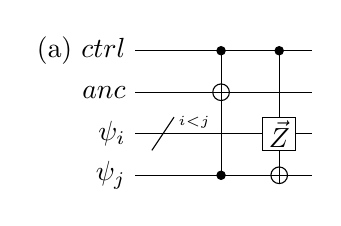
\begin{tikzpicture}[scale=1.000000,x=1pt,y=1pt]
\filldraw[color=white] (0.000000, -7.500000) rectangle (64.000000, 52.500000);
% Drawing wires
% Line 1: ctrl W \text{(a) }ctrl
\draw[color=black] (0.000000,45.000000) -- (64.000000,45.000000);
\draw[color=black] (0.000000,45.000000) node[left] {$\text{(a) }ctrl$};
% Line 2: anc W anc
\draw[color=black] (0.000000,30.000000) -- (64.000000,30.000000);
\draw[color=black] (0.000000,30.000000) node[left] {$anc$};
% Line 3: i W \psi_i
\draw[color=black] (0.000000,15.000000) -- (64.000000,15.000000);
\draw[color=black] (0.000000,15.000000) node[left] {$\psi_i$};
% Line 4: j W \psi_j
\draw[color=black] (0.000000,0.000000) -- (64.000000,0.000000);
\draw[color=black] (0.000000,0.000000) node[left] {$\psi_j$};
% Done with wires; drawing gates
% Line 6: i / ^{i<j}
\draw (6.000000, 9.000000) -- (14.000000, 21.000000);
\draw (12.000000, 18.000000) node[right] {$\scriptstyle{^{i<j}}$};
% Line 7: ctrl anc i j LABEL width=-10
% Line 8: ctrl j +anc
\draw (31.000000,45.000000) -- (31.000000,0.000000);
\filldraw (31.000000, 45.000000) circle(1.500000pt);
\filldraw (31.000000, 0.000000) circle(1.500000pt);
\begin{scope}
\draw[fill=white] (31.000000, 30.000000) circle(3.000000pt);
\clip (31.000000, 30.000000) circle(3.000000pt);
\draw (28.000000, 30.000000) -- (34.000000, 30.000000);
\draw (31.000000, 27.000000) -- (31.000000, 33.000000);
\end{scope}
% Line 10: i G $\vec{Z}$ ctrl +j
\draw (52.000000,45.000000) -- (52.000000,0.000000);
\begin{scope}
\draw[fill=white] (52.000000, 15.000000) +(-45.000000:8.485281pt and 8.485281pt) -- +(45.000000:8.485281pt and 8.485281pt) -- +(135.000000:8.485281pt and 8.485281pt) -- +(225.000000:8.485281pt and 8.485281pt) -- cycle;
\clip (52.000000, 15.000000) +(-45.000000:8.485281pt and 8.485281pt) -- +(45.000000:8.485281pt and 8.485281pt) -- +(135.000000:8.485281pt and 8.485281pt) -- +(225.000000:8.485281pt and 8.485281pt) -- cycle;
\draw (52.000000, 15.000000) node {$\vec{Z}$};
\end{scope}
\filldraw (52.000000, 45.000000) circle(1.500000pt);
\begin{scope}
\draw[fill=white] (52.000000, 0.000000) circle(3.000000pt);
\clip (52.000000, 0.000000) circle(3.000000pt);
\draw (49.000000, 0.000000) -- (55.000000, 0.000000);
\draw (52.000000, -3.000000) -- (52.000000, 3.000000);
\end{scope}
% Done with gates; drawing ending labels
% Done with ending labels; drawing cut lines and comments
% Done with comments
\end{tikzpicture}

        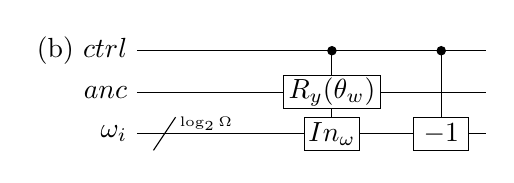
\begin{tikzpicture}[scale=1.000000,x=1pt,y=1pt]
\filldraw[color=white] (0.000000, -7.500000) rectangle (126.000000, 37.500000);
% Drawing wires
% Line 1: ctrl W \text{(b) }ctrl
\draw[color=black] (0.000000,30.000000) -- (126.000000,30.000000);
\draw[color=black] (0.000000,30.000000) node[left] {$\text{(b) }ctrl$};
% Line 2: anc W anc
\draw[color=black] (0.000000,15.000000) -- (126.000000,15.000000);
\draw[color=black] (0.000000,15.000000) node[left] {$anc$};
% Line 3: i W \omega_i
\draw[color=black] (0.000000,0.000000) -- (126.000000,0.000000);
\draw[color=black] (0.000000,0.000000) node[left] {$\omega_i$};
% Done with wires; drawing gates
% Line 5: i / ^{\log_2{\Omega}}
\draw (6.000000, -6.000000) -- (14.000000, 6.000000);
\draw (12.000000, 3.000000) node[right] {$\scriptstyle{^{\log_2{\Omega}}}$};
% Line 6: ctrl anc i LABEL
% Line 8: anc G:width=35 $R_y(\theta_w)$ i G:width=20 $In_\omega$ ctrl
\draw (70.500000,30.000000) -- (70.500000,0.000000);
\begin{scope}
\draw[fill=white] (70.500000, 15.000000) +(-45.000000:24.748737pt and 8.485281pt) -- +(45.000000:24.748737pt and 8.485281pt) -- +(135.000000:24.748737pt and 8.485281pt) -- +(225.000000:24.748737pt and 8.485281pt) -- cycle;
\clip (70.500000, 15.000000) +(-45.000000:24.748737pt and 8.485281pt) -- +(45.000000:24.748737pt and 8.485281pt) -- +(135.000000:24.748737pt and 8.485281pt) -- +(225.000000:24.748737pt and 8.485281pt) -- cycle;
\draw (70.500000, 15.000000) node {$R_y(\theta_w)$};
\end{scope}
\begin{scope}
\draw[fill=white] (70.500000, -0.000000) +(-45.000000:14.142136pt and 8.485281pt) -- +(45.000000:14.142136pt and 8.485281pt) -- +(135.000000:14.142136pt and 8.485281pt) -- +(225.000000:14.142136pt and 8.485281pt) -- cycle;
\clip (70.500000, -0.000000) +(-45.000000:14.142136pt and 8.485281pt) -- +(45.000000:14.142136pt and 8.485281pt) -- +(135.000000:14.142136pt and 8.485281pt) -- +(225.000000:14.142136pt and 8.485281pt) -- cycle;
\draw (70.500000, -0.000000) node {$In_\omega$};
\end{scope}
\filldraw (70.500000, 30.000000) circle(1.500000pt);
% Line 9: i G width=20 $-1$ ctrl
\draw (110.000000,30.000000) -- (110.000000,0.000000);
\begin{scope}
\draw[fill=white] (110.000000, -0.000000) +(-45.000000:14.142136pt and 8.485281pt) -- +(45.000000:14.142136pt and 8.485281pt) -- +(135.000000:14.142136pt and 8.485281pt) -- +(225.000000:14.142136pt and 8.485281pt) -- cycle;
\clip (110.000000, -0.000000) +(-45.000000:14.142136pt and 8.485281pt) -- +(45.000000:14.142136pt and 8.485281pt) -- +(135.000000:14.142136pt and 8.485281pt) -- +(225.000000:14.142136pt and 8.485281pt) -- cycle;
\draw (110.000000, -0.000000) node {$-1$};
\end{scope}
\filldraw (110.000000, 30.000000) circle(1.500000pt);
% Done with gates; drawing ending labels
% Done with ending labels; drawing cut lines and comments
% Done with comments
\end{tikzpicture}

    }
    \caption{
        \textbf{Fermionic Ladder Operator Block-Encodings}
        In subfigure (a), a block-encoding for the fermionic creation operator acting on the $j^\text{th}$ mode is given.
        In subfigure (b), a block-encoding for the fermionic annihilation operator acting on the $j^\text{th}$ mode is given.
        For a creation (annihilation) operator, the branch of the wavefunction will be flipped outside of the encoded subspace if the mode is occupied (unoccupied).
        The state is updated by applying Pauli $Z$ gates to the preceeding fermionic modes which result in the appropriate sign of the state and then by applying a Pauli $X$ gate to flip the occupation of the $j^\text{th}$ mode.
    }
    \label{fig:fermionic-be}
\end{figure}


A construction for $U_{b^\dagger_j}$ is given in subfigure \ref{fig:fermionic-be}a.
The initial Toffoli gate flips the ancilla qubit to indicate that the state has been zeroed-out when the control qubit is on ($\ket{1}$) and the fermionic mode is occupied ($\ket{1}$).
The sign of the output state can be applied appropriately using a series of controlled Pauli $Z$ operators applied to each of the fermionic modes with index $i < j$: $\vec{Z}_i$.
The occupation of the fermionic mode on which the ladder operator acts is updated using a controlled Pauli $X$ operator: $X_j$.

A block-encoding for the fermionic annihilation operator, $U_{b_j}$, can be constructed similarly to $U_{b^\dagger_j}$ and is shown in subfigue \ref{fig:fermionic-be}b.
The fermionic creation operator only acts nontrivially when the mode is \textit{unoccupied}.
Inversely, the fermionic annihilation operator will only act nontrivially if the mode is \textit{occupied}.
Therefore the block-encoding ancilla is flipped outside of the encoded subspace if the control qubit is on ($\ket{1}$) and the fermionic mode is unoccupied ($\ket{0}$).

As noted in Appendix \ref{sec:elbows}, each Toffoli gate can be implemented using 4 T gates and one clean ancilla.
These block-encodings have an optimal rescaling factor ($\lambda = 1$), require one block-encoding ancilla and one clean ancillae, and use four T gates.

\subsection{Products of Fermionic Ladder Operators}

As discussed in subsection \ref{subsec:be-products}, a block-encoding for a product of operators can be constructed using a product of the unitaries that block-encode each operator.
In this subsection, we construct block-encodings for a product of fermionic ladder operators that use fewer quantum resources than are required by this naive strategy.

\begin{figure}[h]
    \mbox{
        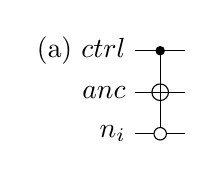
\begin{tikzpicture}[scale=1.000000,x=1pt,y=1pt]
\filldraw[color=white] (0.000000, -7.500000) rectangle (18.000000, 37.500000);
% Drawing wires
% Line 1: ctrl W \text{(a) }ctrl
\draw[color=black] (0.000000,30.000000) -- (18.000000,30.000000);
\draw[color=black] (0.000000,30.000000) node[left] {$\text{(a) }ctrl$};
% Line 2: anc W anc
\draw[color=black] (0.000000,15.000000) -- (18.000000,15.000000);
\draw[color=black] (0.000000,15.000000) node[left] {$anc$};
% Line 3: i W n_i
\draw[color=black] (0.000000,0.000000) -- (18.000000,0.000000);
\draw[color=black] (0.000000,0.000000) node[left] {$n_i$};
% Done with wires; drawing gates
% Line 5: -i +anc ctrl
\draw (9.000000,30.000000) -- (9.000000,0.000000);
\draw[fill=white] (9.000000, 0.000000) circle(2.250000pt);
\begin{scope}
\draw[fill=white] (9.000000, 15.000000) circle(3.000000pt);
\clip (9.000000, 15.000000) circle(3.000000pt);
\draw (6.000000, 15.000000) -- (12.000000, 15.000000);
\draw (9.000000, 12.000000) -- (9.000000, 18.000000);
\end{scope}
\filldraw (9.000000, 30.000000) circle(1.500000pt);
% Done with gates; drawing ending labels
% Done with ending labels; drawing cut lines and comments
% Done with comments
\end{tikzpicture}

        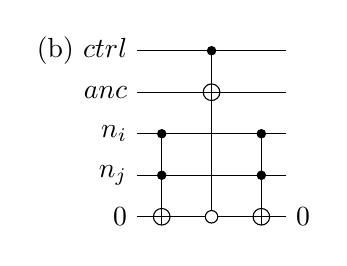
\begin{tikzpicture}[scale=1.000000,x=1pt,y=1pt]
\filldraw[color=white] (0.000000, -7.500000) rectangle (54.000000, 67.500000);
% Drawing wires
% Line 1: ctrl W \text{(b) }ctrl
\draw[color=black] (0.000000,60.000000) -- (54.000000,60.000000);
\draw[color=black] (0.000000,60.000000) node[left] {$\text{(b) }ctrl$};
% Line 2: anc W anc
\draw[color=black] (0.000000,45.000000) -- (54.000000,45.000000);
\draw[color=black] (0.000000,45.000000) node[left] {$anc$};
% Line 3: i W n_i
\draw[color=black] (0.000000,30.000000) -- (54.000000,30.000000);
\draw[color=black] (0.000000,30.000000) node[left] {$n_i$};
% Line 4: j W n_j
\draw[color=black] (0.000000,15.000000) -- (54.000000,15.000000);
\draw[color=black] (0.000000,15.000000) node[left] {$n_j$};
% Line 5: clean0 W 0 0
\draw[color=black] (0.000000,0.000000) -- (54.000000,0.000000);
\draw[color=black] (0.000000,0.000000) node[left] {$0$};
% Done with wires; drawing gates
% Line 7: i j +clean0
\draw (9.000000,30.000000) -- (9.000000,0.000000);
\filldraw (9.000000, 30.000000) circle(1.500000pt);
\filldraw (9.000000, 15.000000) circle(1.500000pt);
\begin{scope}
\draw[fill=white] (9.000000, 0.000000) circle(3.000000pt);
\clip (9.000000, 0.000000) circle(3.000000pt);
\draw (6.000000, 0.000000) -- (12.000000, 0.000000);
\draw (9.000000, -3.000000) -- (9.000000, 3.000000);
\end{scope}
% Line 8: -clean0 ctrl +anc
\draw (27.000000,60.000000) -- (27.000000,0.000000);
\draw[fill=white] (27.000000, 0.000000) circle(2.250000pt);
\filldraw (27.000000, 60.000000) circle(1.500000pt);
\begin{scope}
\draw[fill=white] (27.000000, 45.000000) circle(3.000000pt);
\clip (27.000000, 45.000000) circle(3.000000pt);
\draw (24.000000, 45.000000) -- (30.000000, 45.000000);
\draw (27.000000, 42.000000) -- (27.000000, 48.000000);
\end{scope}
% Line 9: i j +clean0
\draw (45.000000,30.000000) -- (45.000000,0.000000);
\filldraw (45.000000, 30.000000) circle(1.500000pt);
\filldraw (45.000000, 15.000000) circle(1.500000pt);
\begin{scope}
\draw[fill=white] (45.000000, 0.000000) circle(3.000000pt);
\clip (45.000000, 0.000000) circle(3.000000pt);
\draw (42.000000, 0.000000) -- (48.000000, 0.000000);
\draw (45.000000, -3.000000) -- (45.000000, 3.000000);
\end{scope}
% Done with gates; drawing ending labels
\draw[color=black] (54.000000,0.000000) node[right] {$0$};
% Done with ending labels; drawing cut lines and comments
% Done with comments
\end{tikzpicture}

    }
    \mbox{
        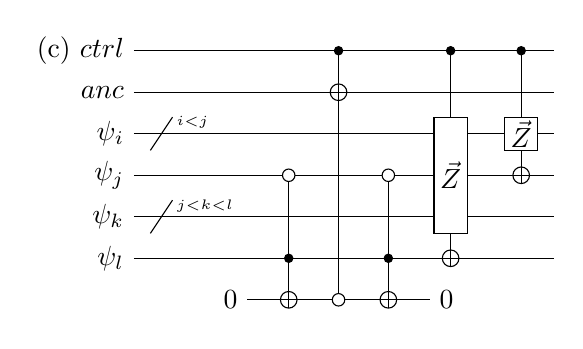
\begin{tikzpicture}[scale=1.000000,x=1pt,y=1pt]
\filldraw[color=white] (0.000000, -7.500000) rectangle (152.000000, 97.500000);
% Drawing wires
% Line 1: ctrl W \text{(c) }ctrl
\draw[color=black] (0.000000,90.000000) -- (152.000000,90.000000);
\draw[color=black] (0.000000,90.000000) node[left] {$\text{(c) }ctrl$};
% Line 2: anc W anc
\draw[color=black] (0.000000,75.000000) -- (152.000000,75.000000);
\draw[color=black] (0.000000,75.000000) node[left] {$anc$};
% Line 3: i W \psi_i
\draw[color=black] (0.000000,60.000000) -- (152.000000,60.000000);
\draw[color=black] (0.000000,60.000000) node[left] {$\psi_i$};
% Line 4: j W \psi_j
\draw[color=black] (0.000000,45.000000) -- (152.000000,45.000000);
\draw[color=black] (0.000000,45.000000) node[left] {$\psi_j$};
% Line 5: k W \psi_k
\draw[color=black] (0.000000,30.000000) -- (152.000000,30.000000);
\draw[color=black] (0.000000,30.000000) node[left] {$\psi_k$};
% Line 6: l W \psi_l
\draw[color=black] (0.000000,15.000000) -- (152.000000,15.000000);
\draw[color=black] (0.000000,15.000000) node[left] {$\psi_l$};
% Line 7: clean0 W 0 0
\draw[color=black] (33.500000,0.000000) -- (114.500000,0.000000);
% Done with wires; drawing gates
% Line 9: i / ^{i<j}
\draw (6.000000, 54.000000) -- (14.000000, 66.000000);
\draw (12.000000, 63.000000) node[right] {$\scriptstyle{^{i<j}}$};
% Line 10: k / ^{j<k<l}
\draw (6.000000, 24.000000) -- (14.000000, 36.000000);
\draw (12.000000, 33.000000) node[right] {$\scriptstyle{^{j<k<l}}$};
% Line 11: ctrl anc i j k l LABEL
% Line 13: clean0 START
\draw[color=black] (41.000000,0.000000) node[fill=white,left,minimum height=15.000000pt,minimum width=15.000000pt,inner sep=0pt] {\phantom{$0$}};
\draw[color=black] (41.000000,0.000000) node[left] {$0$};
% Line 14: -j l +clean0
\draw (56.000000,45.000000) -- (56.000000,0.000000);
\draw[fill=white] (56.000000, 45.000000) circle(2.250000pt);
\filldraw (56.000000, 15.000000) circle(1.500000pt);
\begin{scope}
\draw[fill=white] (56.000000, 0.000000) circle(3.000000pt);
\clip (56.000000, 0.000000) circle(3.000000pt);
\draw (53.000000, 0.000000) -- (59.000000, 0.000000);
\draw (56.000000, -3.000000) -- (56.000000, 3.000000);
\end{scope}
% Line 15: ctrl +anc -clean0
\draw (74.000000,90.000000) -- (74.000000,0.000000);
\filldraw (74.000000, 90.000000) circle(1.500000pt);
\begin{scope}
\draw[fill=white] (74.000000, 75.000000) circle(3.000000pt);
\clip (74.000000, 75.000000) circle(3.000000pt);
\draw (71.000000, 75.000000) -- (77.000000, 75.000000);
\draw (74.000000, 72.000000) -- (74.000000, 78.000000);
\end{scope}
\draw[fill=white] (74.000000, 0.000000) circle(2.250000pt);
% Line 16: -j l +clean0
\draw (92.000000,45.000000) -- (92.000000,0.000000);
\draw[fill=white] (92.000000, 45.000000) circle(2.250000pt);
\filldraw (92.000000, 15.000000) circle(1.500000pt);
\begin{scope}
\draw[fill=white] (92.000000, 0.000000) circle(3.000000pt);
\clip (92.000000, 0.000000) circle(3.000000pt);
\draw (89.000000, 0.000000) -- (95.000000, 0.000000);
\draw (92.000000, -3.000000) -- (92.000000, 3.000000);
\end{scope}
% Line 17: clean0 END
\draw[color=black] (107.000000,0.000000) node[fill=white,right,minimum height=15.000000pt,minimum width=15.000000pt,inner sep=0pt] {\phantom{$0$}};
\draw[color=black] (107.000000,0.000000) node[right] {$0$};
% Line 19: i j k G $\vec{Z}$ +l ctrl
\draw (114.500000,90.000000) -- (114.500000,15.000000);
\begin{scope}
\draw[fill=white] (114.500000, 45.000000) +(-45.000000:8.485281pt and 29.698485pt) -- +(45.000000:8.485281pt and 29.698485pt) -- +(135.000000:8.485281pt and 29.698485pt) -- +(225.000000:8.485281pt and 29.698485pt) -- cycle;
\clip (114.500000, 45.000000) +(-45.000000:8.485281pt and 29.698485pt) -- +(45.000000:8.485281pt and 29.698485pt) -- +(135.000000:8.485281pt and 29.698485pt) -- +(225.000000:8.485281pt and 29.698485pt) -- cycle;
\draw (114.500000, 45.000000) node {$\vec{Z}$};
\end{scope}
\begin{scope}
\draw[fill=white] (114.500000, 15.000000) circle(3.000000pt);
\clip (114.500000, 15.000000) circle(3.000000pt);
\draw (111.500000, 15.000000) -- (117.500000, 15.000000);
\draw (114.500000, 12.000000) -- (114.500000, 18.000000);
\end{scope}
\filldraw (114.500000, 90.000000) circle(1.500000pt);
% Line 20: i G $\vec{Z}$ +j ctrl
\draw (140.000000,90.000000) -- (140.000000,45.000000);
\begin{scope}
\draw[fill=white] (140.000000, 60.000000) +(-45.000000:8.485281pt and 8.485281pt) -- +(45.000000:8.485281pt and 8.485281pt) -- +(135.000000:8.485281pt and 8.485281pt) -- +(225.000000:8.485281pt and 8.485281pt) -- cycle;
\clip (140.000000, 60.000000) +(-45.000000:8.485281pt and 8.485281pt) -- +(45.000000:8.485281pt and 8.485281pt) -- +(135.000000:8.485281pt and 8.485281pt) -- +(225.000000:8.485281pt and 8.485281pt) -- cycle;
\draw (140.000000, 60.000000) node {$\vec{Z}$};
\end{scope}
\begin{scope}
\draw[fill=white] (140.000000, 45.000000) circle(3.000000pt);
\clip (140.000000, 45.000000) circle(3.000000pt);
\draw (137.000000, 45.000000) -- (143.000000, 45.000000);
\draw (140.000000, 42.000000) -- (140.000000, 48.000000);
\end{scope}
\filldraw (140.000000, 90.000000) circle(1.500000pt);
% Done with gates; drawing ending labels
% Done with ending labels; drawing cut lines and comments
% Done with comments
\end{tikzpicture}

        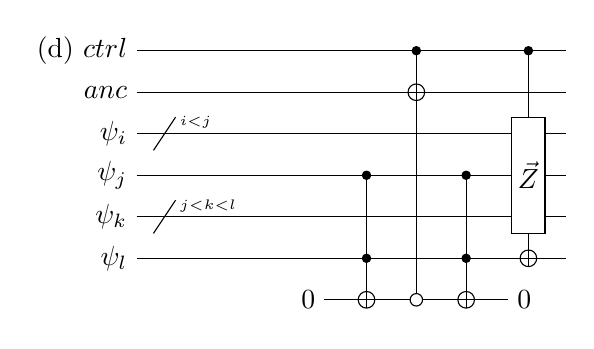
\begin{tikzpicture}[scale=1.000000,x=1pt,y=1pt]
\filldraw[color=white] (0.000000, -7.500000) rectangle (155.000000, 97.500000);
% Drawing wires
% Line 1: ctrl W \text{(d) }ctrl
\draw[color=black] (0.000000,90.000000) -- (155.000000,90.000000);
\draw[color=black] (0.000000,90.000000) node[left] {$\text{(d) }ctrl$};
% Line 2: anc W anc
\draw[color=black] (0.000000,75.000000) -- (155.000000,75.000000);
\draw[color=black] (0.000000,75.000000) node[left] {$anc$};
% Line 3: i W \psi_i
\draw[color=black] (0.000000,60.000000) -- (155.000000,60.000000);
\draw[color=black] (0.000000,60.000000) node[left] {$\psi_i$};
% Line 4: j W \psi_j
\draw[color=black] (0.000000,45.000000) -- (155.000000,45.000000);
\draw[color=black] (0.000000,45.000000) node[left] {$\psi_j$};
% Line 5: k W \psi_k
\draw[color=black] (0.000000,30.000000) -- (155.000000,30.000000);
\draw[color=black] (0.000000,30.000000) node[left] {$\psi_k$};
% Line 6: l W \psi_l
\draw[color=black] (0.000000,15.000000) -- (155.000000,15.000000);
\draw[color=black] (0.000000,15.000000) node[left] {$\psi_l$};
% Line 7: clean0 W 0 0
\draw[color=black] (60.500000,0.000000) -- (141.500000,0.000000);
% Done with wires; drawing gates
% Line 9: i / ^{i<j}
\draw (6.000000, 54.000000) -- (14.000000, 66.000000);
\draw (12.000000, 63.000000) node[right] {$\scriptstyle{^{i<j}}$};
% Line 10: k / ^{j<k<l}
\draw (6.000000, 24.000000) -- (14.000000, 36.000000);
\draw (12.000000, 33.000000) node[right] {$\scriptstyle{^{j<k<l}}$};
% Line 11: ctrl anc i j k l clean0 LABEL
% Line 13: clean0 START
\draw[color=black] (68.000000,0.000000) node[fill=white,left,minimum height=15.000000pt,minimum width=15.000000pt,inner sep=0pt] {\phantom{$0$}};
\draw[color=black] (68.000000,0.000000) node[left] {$0$};
% Line 14: j l +clean0
\draw (83.000000,45.000000) -- (83.000000,0.000000);
\filldraw (83.000000, 45.000000) circle(1.500000pt);
\filldraw (83.000000, 15.000000) circle(1.500000pt);
\begin{scope}
\draw[fill=white] (83.000000, 0.000000) circle(3.000000pt);
\clip (83.000000, 0.000000) circle(3.000000pt);
\draw (80.000000, 0.000000) -- (86.000000, 0.000000);
\draw (83.000000, -3.000000) -- (83.000000, 3.000000);
\end{scope}
% Line 15: ctrl +anc -clean0
\draw (101.000000,90.000000) -- (101.000000,0.000000);
\filldraw (101.000000, 90.000000) circle(1.500000pt);
\begin{scope}
\draw[fill=white] (101.000000, 75.000000) circle(3.000000pt);
\clip (101.000000, 75.000000) circle(3.000000pt);
\draw (98.000000, 75.000000) -- (104.000000, 75.000000);
\draw (101.000000, 72.000000) -- (101.000000, 78.000000);
\end{scope}
\draw[fill=white] (101.000000, 0.000000) circle(2.250000pt);
% Line 16: j l +clean0
\draw (119.000000,45.000000) -- (119.000000,0.000000);
\filldraw (119.000000, 45.000000) circle(1.500000pt);
\filldraw (119.000000, 15.000000) circle(1.500000pt);
\begin{scope}
\draw[fill=white] (119.000000, 0.000000) circle(3.000000pt);
\clip (119.000000, 0.000000) circle(3.000000pt);
\draw (116.000000, 0.000000) -- (122.000000, 0.000000);
\draw (119.000000, -3.000000) -- (119.000000, 3.000000);
\end{scope}
% Line 17: clean0 END
\draw[color=black] (134.000000,0.000000) node[fill=white,right,minimum height=15.000000pt,minimum width=15.000000pt,inner sep=0pt] {\phantom{$0$}};
\draw[color=black] (134.000000,0.000000) node[right] {$0$};
% Line 19: i j k G $\vec{Z}$ +l ctrl
\draw (141.500000,90.000000) -- (141.500000,15.000000);
\begin{scope}
\draw[fill=white] (141.500000, 45.000000) +(-45.000000:8.485281pt and 29.698485pt) -- +(45.000000:8.485281pt and 29.698485pt) -- +(135.000000:8.485281pt and 29.698485pt) -- +(225.000000:8.485281pt and 29.698485pt) -- cycle;
\clip (141.500000, 45.000000) +(-45.000000:8.485281pt and 29.698485pt) -- +(45.000000:8.485281pt and 29.698485pt) -- +(135.000000:8.485281pt and 29.698485pt) -- +(225.000000:8.485281pt and 29.698485pt) -- cycle;
\draw (141.500000, 45.000000) node {$\vec{Z}$};
\end{scope}
\begin{scope}
\draw[fill=white] (141.500000, 15.000000) circle(3.000000pt);
\clip (141.500000, 15.000000) circle(3.000000pt);
\draw (138.500000, 15.000000) -- (144.500000, 15.000000);
\draw (141.500000, 12.000000) -- (141.500000, 18.000000);
\end{scope}
\filldraw (141.500000, 90.000000) circle(1.500000pt);
% Done with gates; drawing ending labels
% Done with ending labels; drawing cut lines and comments
% Done with comments
\end{tikzpicture}

    }
    \caption{
        \textbf{Block-Encoding Products of Fermionic Ladder Operators}
        In subfigure (a), a block-encoding for the fermionic number operator acting on the $i^\text{th}$ mode ($b_i^\dagger b_i$) is given.
        In subfigure (b), a block-encoding for the product of two fermionic number operators acting on the $i^\text{th}$ and $j^\text{th}$ modes ($b_i^\dagger b_i b_j^\dagger b_j$) is given.
        In subfigure (c), a block-encoding for the operator $b_j^\dagger b_l$ with $i \neq l$ is given.
        In subfigure (d), a block-encoding for the operator $b_j^\dagger b_j b_l$ with $i \neq l$ is given.
    }
    \label{fig:fermionic-products-be}
\end{figure}

Consider the action of the fermionic number operator ($b_i^\dagger b_i$):
\begin{equation}
    \begin{split}
        b_i^\dagger b_i \ket{\psi_{b_i}} = \begin{cases} 
            \ket{1} & \text{when $\ket{\psi_{b_i}}$ is $\ket{1}$} \\
            0 & \text{when $\ket{\psi_{b_i}}$ is $\ket{0}$} \\
                                        \end{cases}
    \end{split}
\end{equation}
If the $i^\text{th}$ mode is unoccupied, the state will be zeroed-out.
If the $i^\text{th}$ mode is occupied, then the state is left unchanged.

This action can be encoded using the circuit shown in subfigure \ref{fig:fermionic-products-be}a.
The Toffoli gate flips the block-encoding ancilla outside of the encoded subspace if the control is on and the $i^\text{th}$ mode is unoccupied.
Otherwise, the state of the system and the block-encoding ancilla are left unchanged.
Block-encoding this operator as the product of the block-encodings for $b_i$ and $b_i^\dagger$ would require two block-encoding ancillae and use $8$ T gates.
Meanwhile, this construction has an optimal rescaling factor ($\lambda = 1$), requires one block-encoding ancilla and one clean ancilla, and uses $4$ T gates.

A block-encoding circuit for the operator $b_j^\dagger b_l$ is given in subfigure \ref{fig:fermionic-products-be}c.
For this operator, we can infer that the state will be zeroed-out \textit{unless} both the $j^\text{th}$ mode is unoccupied and the $l^\text{th}$ mode is occupied.
If the control qubit is on and these two conditions are not both true, then the block-encoding ancilla is flipped outside of the encoded subspace.
The state of the system is updated based on the two operators in the order in which they would act upon the quantum state: $\vec{Z}X_l$ ($b_l$) then $\vec{Z}X_j$ ($b_j^\dagger$).
This block-encoding circuit has an optimal rescaling factor ($\lambda = 1$), requires one block-encoding ancilla and two clean ancillae, and uses $8$ T gates.


This construction can be generalized to an arbitrary product of ladder operators.
Let $B$ represent the number of active modes in a term.
Where an ``active mode" is a mode that has a ladder operator applied to it within the current operator.
For example, the term $b_i b_j^\dagger b_k b_l^\dagger b_l$ has $4$ active modes.
Each active mode will contribute a new control condition on the state of the corresponding mode.
Therefore, a block-encoding circuit for a general product of fermionic ladder operators with $B$ active modes will have an optimal rescaling factor ($\lambda = 1$), require one block-encoding ancilla and $B$ clean ancillae, and use $4B$ T gates.

% \ws{
% A natural question to ask is how do these constructions compare with using an LCU block-encoding after applying the Jordan-Wigner transformation \cite{}?
% The Jordan-Wigner transformation maps each fermionic ladder operator (or number operator) to a sum of two Pauli operators.
% For an arbitrary product of fermionic ladder operators, expanding these linear combinations results in $2^{B}$ Paulis.
% The number of non-Clifford gates for LCU scales linearly with the number of operators and hence would scale exponentially with $B$ under this construction.
% Alternatively, one could construct LCU block-encodings for each of the ladder operators in a term by applying the Jordan-Wigner transformation to each ladder operator (or number operator) independently.
% The product of these block-encodings would then give a block-encoding of the term.
% For each ladder operator (or number operator), an LCU block-encoding would require one Toffoli gate and one ancilla qubit.
% A block-encoding of the whole term using this construction would then require $B$ Toffoli gates and $B$ block-encoding ancillae.
% }

\subsection{Linear Combinations of Fermionic Ladder Operators}


As discussed in subsection \ref{subsec:lco}, a block-encoding for a linear combination of operators can be constructed using the LCO framework.
In this subsection, we show how to construct block-encodings of linear combinations of products of fermionic ladder operators that use fewer quantum resources than are required by an LCO construction.
In particular, we give a generalized construction for a product of fermionic ladder operators plus its hermitian conjugate, however, we note that the strategies we present here are not restricted to hermitian conjugates.

\begin{figure}
    \mbox{
        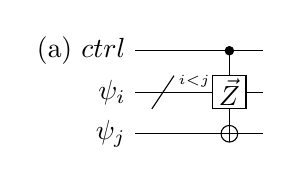
\begin{tikzpicture}[scale=1.000000,x=1pt,y=1pt]
\filldraw[color=white] (0.000000, -7.500000) rectangle (46.000000, 37.500000);
% Drawing wires
% Line 1: a W \text{(a) }ctrl
\draw[color=black] (0.000000,30.000000) -- (46.000000,30.000000);
\draw[color=black] (0.000000,30.000000) node[left] {$\text{(a) }ctrl$};
% Line 2: b W \psi_i
\draw[color=black] (0.000000,15.000000) -- (46.000000,15.000000);
\draw[color=black] (0.000000,15.000000) node[left] {$\psi_i$};
% Line 3: c W \psi_j
\draw[color=black] (0.000000,0.000000) -- (46.000000,0.000000);
\draw[color=black] (0.000000,0.000000) node[left] {$\psi_j$};
% Done with wires; drawing gates
% Line 5: b / ^{i<j}
\draw (6.000000, 9.000000) -- (14.000000, 21.000000);
\draw (12.000000, 18.000000) node[right] {$\scriptstyle{^{i<j}}$};
% Line 6: a b c LABEL width=-10
% Line 7: b G $\vec{Z}$ a +c
\draw (34.000000,30.000000) -- (34.000000,0.000000);
\begin{scope}
\draw[fill=white] (34.000000, 15.000000) +(-45.000000:8.485281pt and 8.485281pt) -- +(45.000000:8.485281pt and 8.485281pt) -- +(135.000000:8.485281pt and 8.485281pt) -- +(225.000000:8.485281pt and 8.485281pt) -- cycle;
\clip (34.000000, 15.000000) +(-45.000000:8.485281pt and 8.485281pt) -- +(45.000000:8.485281pt and 8.485281pt) -- +(135.000000:8.485281pt and 8.485281pt) -- +(225.000000:8.485281pt and 8.485281pt) -- cycle;
\draw (34.000000, 15.000000) node {$\vec{Z}$};
\end{scope}
\filldraw (34.000000, 30.000000) circle(1.500000pt);
\begin{scope}
\draw[fill=white] (34.000000, 0.000000) circle(3.000000pt);
\clip (34.000000, 0.000000) circle(3.000000pt);
\draw (31.000000, 0.000000) -- (37.000000, 0.000000);
\draw (34.000000, -3.000000) -- (34.000000, 3.000000);
\end{scope}
% Done with gates; drawing ending labels
% Done with ending labels; drawing cut lines and comments
% Done with comments
\end{tikzpicture}

        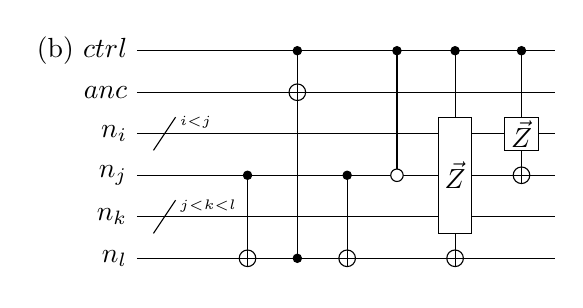
\begin{tikzpicture}[scale=1.000000,x=1pt,y=1pt]
\filldraw[color=white] (0.000000, -7.500000) rectangle (151.000000, 82.500000);
% Drawing wires
% Line 1: c W \text{(b) }ctrl
\draw[color=black] (0.000000,75.000000) -- (151.000000,75.000000);
\draw[color=black] (0.000000,75.000000) node[left] {$\text{(b) }ctrl$};
% Line 2: a W anc
\draw[color=black] (0.000000,60.000000) -- (151.000000,60.000000);
\draw[color=black] (0.000000,60.000000) node[left] {$anc$};
% Line 3: i W n_i
\draw[color=black] (0.000000,45.000000) -- (151.000000,45.000000);
\draw[color=black] (0.000000,45.000000) node[left] {$n_i$};
% Line 4: j W n_j
\draw[color=black] (0.000000,30.000000) -- (151.000000,30.000000);
\draw[color=black] (0.000000,30.000000) node[left] {$n_j$};
% Line 5: k W n_k
\draw[color=black] (0.000000,15.000000) -- (151.000000,15.000000);
\draw[color=black] (0.000000,15.000000) node[left] {$n_k$};
% Line 6: l W n_l
\draw[color=black] (0.000000,0.000000) -- (151.000000,0.000000);
\draw[color=black] (0.000000,0.000000) node[left] {$n_l$};
% Done with wires; drawing gates
% Line 8: i / ^{i<j}
\draw (6.000000, 39.000000) -- (14.000000, 51.000000);
\draw (12.000000, 48.000000) node[right] {$\scriptstyle{^{i<j}}$};
% Line 9: k / ^{j<k<l}
\draw (6.000000, 9.000000) -- (14.000000, 21.000000);
\draw (12.000000, 18.000000) node[right] {$\scriptstyle{^{j<k<l}}$};
% Line 10: c a i j k l LABEL width=-1
% Line 11: j +l
\draw (40.000000,30.000000) -- (40.000000,0.000000);
\filldraw (40.000000, 30.000000) circle(1.500000pt);
\begin{scope}
\draw[fill=white] (40.000000, 0.000000) circle(3.000000pt);
\clip (40.000000, 0.000000) circle(3.000000pt);
\draw (37.000000, 0.000000) -- (43.000000, 0.000000);
\draw (40.000000, -3.000000) -- (40.000000, 3.000000);
\end{scope}
% Line 12: c l +a
\draw (58.000000,75.000000) -- (58.000000,0.000000);
\filldraw (58.000000, 75.000000) circle(1.500000pt);
\filldraw (58.000000, 0.000000) circle(1.500000pt);
\begin{scope}
\draw[fill=white] (58.000000, 60.000000) circle(3.000000pt);
\clip (58.000000, 60.000000) circle(3.000000pt);
\draw (55.000000, 60.000000) -- (61.000000, 60.000000);
\draw (58.000000, 57.000000) -- (58.000000, 63.000000);
\end{scope}
% Line 13: j +l
\draw (76.000000,30.000000) -- (76.000000,0.000000);
\filldraw (76.000000, 30.000000) circle(1.500000pt);
\begin{scope}
\draw[fill=white] (76.000000, 0.000000) circle(3.000000pt);
\clip (76.000000, 0.000000) circle(3.000000pt);
\draw (73.000000, 0.000000) -- (79.000000, 0.000000);
\draw (76.000000, -3.000000) -- (76.000000, 3.000000);
\end{scope}
% Line 14: c -j
\draw (94.000000,75.000000) -- (94.000000,30.000000);
\filldraw (94.000000, 75.000000) circle(1.500000pt);
\draw[fill=white] (94.000000, 30.000000) circle(2.250000pt);
% Line 16: i j k G $\vec{Z}$ c +l
\draw (115.000000,75.000000) -- (115.000000,0.000000);
\begin{scope}
\draw[fill=white] (115.000000, 30.000000) +(-45.000000:8.485281pt and 29.698485pt) -- +(45.000000:8.485281pt and 29.698485pt) -- +(135.000000:8.485281pt and 29.698485pt) -- +(225.000000:8.485281pt and 29.698485pt) -- cycle;
\clip (115.000000, 30.000000) +(-45.000000:8.485281pt and 29.698485pt) -- +(45.000000:8.485281pt and 29.698485pt) -- +(135.000000:8.485281pt and 29.698485pt) -- +(225.000000:8.485281pt and 29.698485pt) -- cycle;
\draw (115.000000, 30.000000) node {$\vec{Z}$};
\end{scope}
\filldraw (115.000000, 75.000000) circle(1.500000pt);
\begin{scope}
\draw[fill=white] (115.000000, 0.000000) circle(3.000000pt);
\clip (115.000000, 0.000000) circle(3.000000pt);
\draw (112.000000, 0.000000) -- (118.000000, 0.000000);
\draw (115.000000, -3.000000) -- (115.000000, 3.000000);
\end{scope}
% Line 17: i G $\vec{Z}$ c +j
\draw (139.000000,75.000000) -- (139.000000,30.000000);
\begin{scope}
\draw[fill=white] (139.000000, 45.000000) +(-45.000000:8.485281pt and 8.485281pt) -- +(45.000000:8.485281pt and 8.485281pt) -- +(135.000000:8.485281pt and 8.485281pt) -- +(225.000000:8.485281pt and 8.485281pt) -- cycle;
\clip (139.000000, 45.000000) +(-45.000000:8.485281pt and 8.485281pt) -- +(45.000000:8.485281pt and 8.485281pt) -- +(135.000000:8.485281pt and 8.485281pt) -- +(225.000000:8.485281pt and 8.485281pt) -- cycle;
\draw (139.000000, 45.000000) node {$\vec{Z}$};
\end{scope}
\filldraw (139.000000, 75.000000) circle(1.500000pt);
\begin{scope}
\draw[fill=white] (139.000000, 30.000000) circle(3.000000pt);
\clip (139.000000, 30.000000) circle(3.000000pt);
\draw (136.000000, 30.000000) -- (142.000000, 30.000000);
\draw (139.000000, 27.000000) -- (139.000000, 33.000000);
\end{scope}
% Done with gates; drawing ending labels
% Done with ending labels; drawing cut lines and comments
% Done with comments
\end{tikzpicture}

    }
    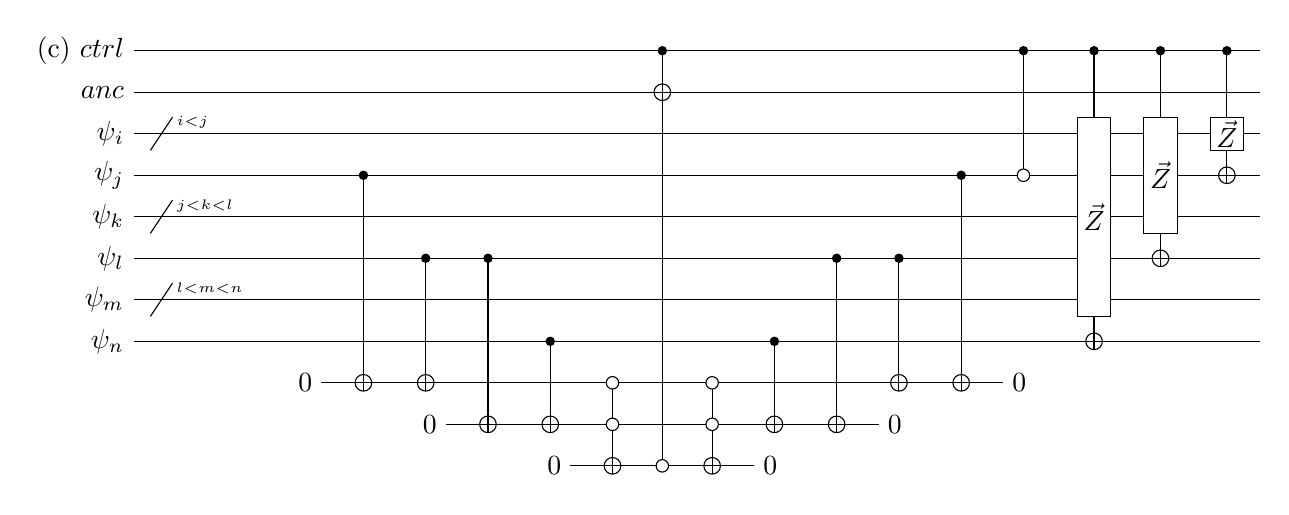
\begin{tikzpicture}[scale=1.000000,x=1pt,y=1pt]
\filldraw[color=white] (0.000000, -7.500000) rectangle (407.000000, 157.500000);
% Drawing wires
% Line 1: ctrl W \text{(c) }ctrl
\draw[color=black] (0.000000,150.000000) -- (407.000000,150.000000);
\draw[color=black] (0.000000,150.000000) node[left] {$\text{(c) }ctrl$};
% Line 2: anc W anc
\draw[color=black] (0.000000,135.000000) -- (407.000000,135.000000);
\draw[color=black] (0.000000,135.000000) node[left] {$anc$};
% Line 3: i W \psi_i
\draw[color=black] (0.000000,120.000000) -- (407.000000,120.000000);
\draw[color=black] (0.000000,120.000000) node[left] {$\psi_i$};
% Line 4: j W \psi_j
\draw[color=black] (0.000000,105.000000) -- (407.000000,105.000000);
\draw[color=black] (0.000000,105.000000) node[left] {$\psi_j$};
% Line 5: k W \psi_k
\draw[color=black] (0.000000,90.000000) -- (407.000000,90.000000);
\draw[color=black] (0.000000,90.000000) node[left] {$\psi_k$};
% Line 6: l W \psi_l
\draw[color=black] (0.000000,75.000000) -- (407.000000,75.000000);
\draw[color=black] (0.000000,75.000000) node[left] {$\psi_l$};
% Line 7: m W \psi_m
\draw[color=black] (0.000000,60.000000) -- (407.000000,60.000000);
\draw[color=black] (0.000000,60.000000) node[left] {$\psi_m$};
% Line 8: n W \psi_n
\draw[color=black] (0.000000,45.000000) -- (407.000000,45.000000);
\draw[color=black] (0.000000,45.000000) node[left] {$\psi_n$};
% Line 9: clean0 W 0 0
\draw[color=black] (60.500000,30.000000) -- (321.500000,30.000000);
% Line 10: clean1 W 0 0
\draw[color=black] (105.500000,15.000000) -- (276.500000,15.000000);
% Line 11: clean2 W 0 0
\draw[color=black] (150.500000,0.000000) -- (231.500000,0.000000);
% Done with wires; drawing gates
% Line 13: i / ^{i<j}
\draw (6.000000, 114.000000) -- (14.000000, 126.000000);
\draw (12.000000, 123.000000) node[right] {$\scriptstyle{^{i<j}}$};
% Line 14: k / ^{j<k<l}
\draw (6.000000, 84.000000) -- (14.000000, 96.000000);
\draw (12.000000, 93.000000) node[right] {$\scriptstyle{^{j<k<l}}$};
% Line 15: m / ^{l<m<n}
\draw (6.000000, 54.000000) -- (14.000000, 66.000000);
\draw (12.000000, 63.000000) node[right] {$\scriptstyle{^{l<m<n}}$};
% Line 16: ctrl anc i j k l m n clean0 LABEL
% Line 17: clean0 START
\draw[color=black] (68.000000,30.000000) node[fill=white,left,minimum height=15.000000pt,minimum width=15.000000pt,inner sep=0pt] {\phantom{$0$}};
\draw[color=black] (68.000000,30.000000) node[left] {$0$};
% Line 18: j +clean0
\draw (83.000000,105.000000) -- (83.000000,30.000000);
\filldraw (83.000000, 105.000000) circle(1.500000pt);
\begin{scope}
\draw[fill=white] (83.000000, 30.000000) circle(3.000000pt);
\clip (83.000000, 30.000000) circle(3.000000pt);
\draw (80.000000, 30.000000) -- (86.000000, 30.000000);
\draw (83.000000, 27.000000) -- (83.000000, 33.000000);
\end{scope}
% Line 19: l +clean0
\draw (105.500000,75.000000) -- (105.500000,30.000000);
\filldraw (105.500000, 75.000000) circle(1.500000pt);
\begin{scope}
\draw[fill=white] (105.500000, 30.000000) circle(3.000000pt);
\clip (105.500000, 30.000000) circle(3.000000pt);
\draw (102.500000, 30.000000) -- (108.500000, 30.000000);
\draw (105.500000, 27.000000) -- (105.500000, 33.000000);
\end{scope}
% Line 20: clean1 START
\draw[color=black] (113.000000,15.000000) node[fill=white,left,minimum height=15.000000pt,minimum width=15.000000pt,inner sep=0pt] {\phantom{$0$}};
\draw[color=black] (113.000000,15.000000) node[left] {$0$};
% Line 21: l +clean1
\draw (128.000000,75.000000) -- (128.000000,15.000000);
\filldraw (128.000000, 75.000000) circle(1.500000pt);
\begin{scope}
\draw[fill=white] (128.000000, 15.000000) circle(3.000000pt);
\clip (128.000000, 15.000000) circle(3.000000pt);
\draw (125.000000, 15.000000) -- (131.000000, 15.000000);
\draw (128.000000, 12.000000) -- (128.000000, 18.000000);
\end{scope}
% Line 22: n +clean1
\draw (150.500000,45.000000) -- (150.500000,15.000000);
\filldraw (150.500000, 45.000000) circle(1.500000pt);
\begin{scope}
\draw[fill=white] (150.500000, 15.000000) circle(3.000000pt);
\clip (150.500000, 15.000000) circle(3.000000pt);
\draw (147.500000, 15.000000) -- (153.500000, 15.000000);
\draw (150.500000, 12.000000) -- (150.500000, 18.000000);
\end{scope}
% Line 23: clean2 START
\draw[color=black] (158.000000,0.000000) node[fill=white,left,minimum height=15.000000pt,minimum width=15.000000pt,inner sep=0pt] {\phantom{$0$}};
\draw[color=black] (158.000000,0.000000) node[left] {$0$};
% Line 24: -clean0 -clean1 +clean2
\draw (173.000000,30.000000) -- (173.000000,0.000000);
\draw[fill=white] (173.000000, 30.000000) circle(2.250000pt);
\draw[fill=white] (173.000000, 15.000000) circle(2.250000pt);
\begin{scope}
\draw[fill=white] (173.000000, 0.000000) circle(3.000000pt);
\clip (173.000000, 0.000000) circle(3.000000pt);
\draw (170.000000, 0.000000) -- (176.000000, 0.000000);
\draw (173.000000, -3.000000) -- (173.000000, 3.000000);
\end{scope}
% Line 25: ctrl -clean2 +anc
\draw (191.000000,150.000000) -- (191.000000,0.000000);
\filldraw (191.000000, 150.000000) circle(1.500000pt);
\draw[fill=white] (191.000000, 0.000000) circle(2.250000pt);
\begin{scope}
\draw[fill=white] (191.000000, 135.000000) circle(3.000000pt);
\clip (191.000000, 135.000000) circle(3.000000pt);
\draw (188.000000, 135.000000) -- (194.000000, 135.000000);
\draw (191.000000, 132.000000) -- (191.000000, 138.000000);
\end{scope}
% Line 26: -clean0 -clean1 +clean2
\draw (209.000000,30.000000) -- (209.000000,0.000000);
\draw[fill=white] (209.000000, 30.000000) circle(2.250000pt);
\draw[fill=white] (209.000000, 15.000000) circle(2.250000pt);
\begin{scope}
\draw[fill=white] (209.000000, 0.000000) circle(3.000000pt);
\clip (209.000000, 0.000000) circle(3.000000pt);
\draw (206.000000, 0.000000) -- (212.000000, 0.000000);
\draw (209.000000, -3.000000) -- (209.000000, 3.000000);
\end{scope}
% Line 27: clean2 END
\draw[color=black] (224.000000,0.000000) node[fill=white,right,minimum height=15.000000pt,minimum width=15.000000pt,inner sep=0pt] {\phantom{$0$}};
\draw[color=black] (224.000000,0.000000) node[right] {$0$};
% Line 28: n +clean1
\draw (231.500000,45.000000) -- (231.500000,15.000000);
\filldraw (231.500000, 45.000000) circle(1.500000pt);
\begin{scope}
\draw[fill=white] (231.500000, 15.000000) circle(3.000000pt);
\clip (231.500000, 15.000000) circle(3.000000pt);
\draw (228.500000, 15.000000) -- (234.500000, 15.000000);
\draw (231.500000, 12.000000) -- (231.500000, 18.000000);
\end{scope}
% Line 29: l +clean1
\draw (254.000000,75.000000) -- (254.000000,15.000000);
\filldraw (254.000000, 75.000000) circle(1.500000pt);
\begin{scope}
\draw[fill=white] (254.000000, 15.000000) circle(3.000000pt);
\clip (254.000000, 15.000000) circle(3.000000pt);
\draw (251.000000, 15.000000) -- (257.000000, 15.000000);
\draw (254.000000, 12.000000) -- (254.000000, 18.000000);
\end{scope}
% Line 30: clean1 END
\draw[color=black] (269.000000,15.000000) node[fill=white,right,minimum height=15.000000pt,minimum width=15.000000pt,inner sep=0pt] {\phantom{$0$}};
\draw[color=black] (269.000000,15.000000) node[right] {$0$};
% Line 31: l +clean0
\draw (276.500000,75.000000) -- (276.500000,30.000000);
\filldraw (276.500000, 75.000000) circle(1.500000pt);
\begin{scope}
\draw[fill=white] (276.500000, 30.000000) circle(3.000000pt);
\clip (276.500000, 30.000000) circle(3.000000pt);
\draw (273.500000, 30.000000) -- (279.500000, 30.000000);
\draw (276.500000, 27.000000) -- (276.500000, 33.000000);
\end{scope}
% Line 32: j +clean0
\draw (299.000000,105.000000) -- (299.000000,30.000000);
\filldraw (299.000000, 105.000000) circle(1.500000pt);
\begin{scope}
\draw[fill=white] (299.000000, 30.000000) circle(3.000000pt);
\clip (299.000000, 30.000000) circle(3.000000pt);
\draw (296.000000, 30.000000) -- (302.000000, 30.000000);
\draw (299.000000, 27.000000) -- (299.000000, 33.000000);
\end{scope}
% Line 33: clean0 END
\draw[color=black] (314.000000,30.000000) node[fill=white,right,minimum height=15.000000pt,minimum width=15.000000pt,inner sep=0pt] {\phantom{$0$}};
\draw[color=black] (314.000000,30.000000) node[right] {$0$};
% Line 35: ctrl -j
\draw (321.500000,150.000000) -- (321.500000,105.000000);
\filldraw (321.500000, 150.000000) circle(1.500000pt);
\draw[fill=white] (321.500000, 105.000000) circle(2.250000pt);
% Line 37: i j k l m G $\vec{Z}$ ctrl +n
\draw (347.000000,150.000000) -- (347.000000,45.000000);
\begin{scope}
\draw[fill=white] (347.000000, 90.000000) +(-45.000000:8.485281pt and 50.911688pt) -- +(45.000000:8.485281pt and 50.911688pt) -- +(135.000000:8.485281pt and 50.911688pt) -- +(225.000000:8.485281pt and 50.911688pt) -- cycle;
\clip (347.000000, 90.000000) +(-45.000000:8.485281pt and 50.911688pt) -- +(45.000000:8.485281pt and 50.911688pt) -- +(135.000000:8.485281pt and 50.911688pt) -- +(225.000000:8.485281pt and 50.911688pt) -- cycle;
\draw (347.000000, 90.000000) node {$\vec{Z}$};
\end{scope}
\filldraw (347.000000, 150.000000) circle(1.500000pt);
\begin{scope}
\draw[fill=white] (347.000000, 45.000000) circle(3.000000pt);
\clip (347.000000, 45.000000) circle(3.000000pt);
\draw (344.000000, 45.000000) -- (350.000000, 45.000000);
\draw (347.000000, 42.000000) -- (347.000000, 48.000000);
\end{scope}
% Line 38: i j k G $\vec{Z}$ ctrl +l
\draw (371.000000,150.000000) -- (371.000000,75.000000);
\begin{scope}
\draw[fill=white] (371.000000, 105.000000) +(-45.000000:8.485281pt and 29.698485pt) -- +(45.000000:8.485281pt and 29.698485pt) -- +(135.000000:8.485281pt and 29.698485pt) -- +(225.000000:8.485281pt and 29.698485pt) -- cycle;
\clip (371.000000, 105.000000) +(-45.000000:8.485281pt and 29.698485pt) -- +(45.000000:8.485281pt and 29.698485pt) -- +(135.000000:8.485281pt and 29.698485pt) -- +(225.000000:8.485281pt and 29.698485pt) -- cycle;
\draw (371.000000, 105.000000) node {$\vec{Z}$};
\end{scope}
\filldraw (371.000000, 150.000000) circle(1.500000pt);
\begin{scope}
\draw[fill=white] (371.000000, 75.000000) circle(3.000000pt);
\clip (371.000000, 75.000000) circle(3.000000pt);
\draw (368.000000, 75.000000) -- (374.000000, 75.000000);
\draw (371.000000, 72.000000) -- (371.000000, 78.000000);
\end{scope}
% Line 39: i G $\vec{Z}$ ctrl +j
\draw (395.000000,150.000000) -- (395.000000,105.000000);
\begin{scope}
\draw[fill=white] (395.000000, 120.000000) +(-45.000000:8.485281pt and 8.485281pt) -- +(45.000000:8.485281pt and 8.485281pt) -- +(135.000000:8.485281pt and 8.485281pt) -- +(225.000000:8.485281pt and 8.485281pt) -- cycle;
\clip (395.000000, 120.000000) +(-45.000000:8.485281pt and 8.485281pt) -- +(45.000000:8.485281pt and 8.485281pt) -- +(135.000000:8.485281pt and 8.485281pt) -- +(225.000000:8.485281pt and 8.485281pt) -- cycle;
\draw (395.000000, 120.000000) node {$\vec{Z}$};
\end{scope}
\filldraw (395.000000, 150.000000) circle(1.500000pt);
\begin{scope}
\draw[fill=white] (395.000000, 105.000000) circle(3.000000pt);
\clip (395.000000, 105.000000) circle(3.000000pt);
\draw (392.000000, 105.000000) -- (398.000000, 105.000000);
\draw (395.000000, 102.000000) -- (395.000000, 108.000000);
\end{scope}
% Done with gates; drawing ending labels
% Done with ending labels; drawing cut lines and comments
% Done with comments
\end{tikzpicture}

    \caption{
        \textbf{Block-Encoding Product of Fermionic Operators Plus Hermitian Conjugate}
        In subfigure (a), a block-encoding for the operator $b_j + b_j^\dagger$ is given.
        In subfigure (b), a block-encoding for the operator $b_j b_l + b_l^\dagger b_j^\dagger$ is given.
        In subfigure (c), a block-encoding for the operator $b_j b_l b_n + b_n^\dagger b_l^\dagger b_j^\dagger$ is given.
    }
    \label{fig:fermionic-be-lc-small}
\end{figure}


Consider a linear combination of an individual fermionic ladder operator with its hermitian conjugate: $b_j^\dagger + b_j$.
The action of this operator on the two possible occupation states of the $j^\text{th}$ fermionic mode is given by:
\begin{equation}
    \label{eq:action-of-fermionic-op-plus-hc}
    \begin{split}
        (b_j^\dagger + b_j) \ket{\psi_{b_j}} = \begin{cases} 
            \ket{1} & \text{when $\ket{\psi_{b_j}}$ is $\ket{0}$} \\
            \ket{0} & \text{when $\ket{\psi_{b_j}}$ is $\ket{1}$} \\
                                        \end{cases}
    \end{split}
\end{equation}
The sign flip depending on the parity of the occupation of the preceeding fermionic modes is omitted for brevity.

An LCO construction using the block-encodings for these two ladder operators presented in the previous section would have a rescaling factor of $\lambda = 2$, require two block-encoding ancillae and two clean ancillae, and use $12$ T gates.
However, by considering the action of this operator (Eq. \ref{eq:action-of-fermionic-op-plus-hc}) on the active mode, a more efficient block-encoding can be constructed.
A Pauli $X$ gate can be applied to the $j^\text{th}$ mode to flip the occupation and a string of Pauli $Z$ gates can be applied on each fermionic mode with index $i < j$ to apply the appropriate sign.
This results in the same decomposition one would arrive at using the Jordan-Wigner transformation ($\vec{Z}X_j$).
A circuit diagram for this block-encoding is shown in subfigure \ref{fig:fermionic-be-lc-small}a.
This block-encoding circuit has an optimal rescaling factor ($\lambda = 1$), requires zero block-encoding ancillae and zero clean ancillae, and uses zero non-Clifford operations.

For a two-body fermionic operator and its hermitian conjugate ($b_j b_l + b_l^\dagger b_j^\dagger$) we arrive at a construction that differs from the Jordan-Wigner transformation.
We begin by swapping the operators in the second term using the anticommutation relations to ensure that the order in which the corresponding operators appear in each term is the same: $b_j b_l - b_j^\dagger b_l^\dagger$.
In the circuit, the order in which the system is updated based on the ladder operators is fixed so it must be consistent for both terms.
The action of the joined operator on the possible occupation states of the $i^\text{th}$ and $j^\text{th}$ fermionic modes is given by:
\begin{equation}
    \begin{split}
        (b_j b_l - b_j^\dagger b_l^\dagger) \ket{\psi_{b_j}, \psi_{b_l}} = \begin{cases} 
            \hspace{1em}\ket{11} & \text{when $\ket{\psi_{b_j}, \psi_{b_l}}$ is $\ket{00}$} \\
            -\ket{00} & \text{when $\ket{\psi_{b_j}, \psi_{b_l}}$ is $\ket{11}$} \\
                                        \end{cases}
    \end{split}
\end{equation}
The additional sign flip caused by the parity of the preceeding modes will be consistent for both terms since the order at which the operators appear in each term is consistent.
The action of this operator on the system is determined by the parity of the two fermionic modes.
The state will be zeroed-out by the operator \textit{unless} $\ket{\psi_{b_j}} \oplus \ket{\psi_{b_l}} = \ket{0}$.

In subfigure \ref{fig:fermionic-be-lc-small}b, we give a circuit diagram for block-encoding this two-body operator.
The parity of the active modes can be computed using a CNOT gate controlled on the $j^\text{th}$ mode, targeting the $l^\text{th}$ mode.
If the control qubit is on and $\ket{\psi_{b_l}}$ is in the $\ket{1}$ state (odd parity), then the block-encoding ancilla is flipped to push that branch of the wavefunction outside of the encoded subspace.
After this operation, the parity can be uncomputed, returning the qubit storing the occupation of the $l^\text{th}$ mode to its original state.
Next, a $CZ$ gate that is $0$-controlled on the $j^\text{th}$ fermionic mode and $1$-controlled on the control qubit applies the desired sign flip onto the state corresponding to the term $- b_j^\dagger b_l^\dagger$.
Lastly, a series of $\vec{Z}X$ operators are applied to each active mode in the order at which the operators would be applied onto the system (right to left).

\begin{figure}
    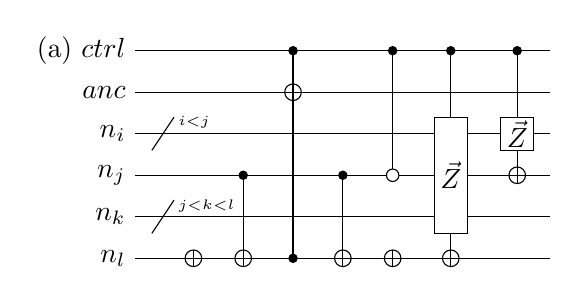
\begin{tikzpicture}[scale=1.000000,x=1pt,y=1pt]
\filldraw[color=white] (0.000000, -7.500000) rectangle (150.000000, 82.500000);
% Drawing wires
% Line 1: c W \text{(a) }ctrl
\draw[color=black] (0.000000,75.000000) -- (150.000000,75.000000);
\draw[color=black] (0.000000,75.000000) node[left] {$\text{(a) }ctrl$};
% Line 2: a W anc
\draw[color=black] (0.000000,60.000000) -- (150.000000,60.000000);
\draw[color=black] (0.000000,60.000000) node[left] {$anc$};
% Line 3: i W n_i
\draw[color=black] (0.000000,45.000000) -- (150.000000,45.000000);
\draw[color=black] (0.000000,45.000000) node[left] {$n_i$};
% Line 4: j W n_j
\draw[color=black] (0.000000,30.000000) -- (150.000000,30.000000);
\draw[color=black] (0.000000,30.000000) node[left] {$n_j$};
% Line 5: k W n_k
\draw[color=black] (0.000000,15.000000) -- (150.000000,15.000000);
\draw[color=black] (0.000000,15.000000) node[left] {$n_k$};
% Line 6: l W n_l
\draw[color=black] (0.000000,0.000000) -- (150.000000,0.000000);
\draw[color=black] (0.000000,0.000000) node[left] {$n_l$};
% Done with wires; drawing gates
% Line 8: i / ^{i<j}
\draw (6.000000, 39.000000) -- (14.000000, 51.000000);
\draw (12.000000, 48.000000) node[right] {$\scriptstyle{^{i<j}}$};
% Line 9: k / ^{j<k<l}
\draw (6.000000, 9.000000) -- (14.000000, 21.000000);
\draw (12.000000, 18.000000) node[right] {$\scriptstyle{^{j<k<l}}$};
% Line 10: c a i j k l LABEL width=-20
% Line 12: +l
\begin{scope}
\draw[fill=white] (21.000000, 0.000000) circle(3.000000pt);
\clip (21.000000, 0.000000) circle(3.000000pt);
\draw (18.000000, 0.000000) -- (24.000000, 0.000000);
\draw (21.000000, -3.000000) -- (21.000000, 3.000000);
\end{scope}
% Line 13: j +l
\draw (39.000000,30.000000) -- (39.000000,0.000000);
\filldraw (39.000000, 30.000000) circle(1.500000pt);
\begin{scope}
\draw[fill=white] (39.000000, 0.000000) circle(3.000000pt);
\clip (39.000000, 0.000000) circle(3.000000pt);
\draw (36.000000, 0.000000) -- (42.000000, 0.000000);
\draw (39.000000, -3.000000) -- (39.000000, 3.000000);
\end{scope}
% Line 14: c l +a
\draw (57.000000,75.000000) -- (57.000000,0.000000);
\filldraw (57.000000, 75.000000) circle(1.500000pt);
\filldraw (57.000000, 0.000000) circle(1.500000pt);
\begin{scope}
\draw[fill=white] (57.000000, 60.000000) circle(3.000000pt);
\clip (57.000000, 60.000000) circle(3.000000pt);
\draw (54.000000, 60.000000) -- (60.000000, 60.000000);
\draw (57.000000, 57.000000) -- (57.000000, 63.000000);
\end{scope}
% Line 15: j +l
\draw (75.000000,30.000000) -- (75.000000,0.000000);
\filldraw (75.000000, 30.000000) circle(1.500000pt);
\begin{scope}
\draw[fill=white] (75.000000, 0.000000) circle(3.000000pt);
\clip (75.000000, 0.000000) circle(3.000000pt);
\draw (72.000000, 0.000000) -- (78.000000, 0.000000);
\draw (75.000000, -3.000000) -- (75.000000, 3.000000);
\end{scope}
% Line 16: +l
\begin{scope}
\draw[fill=white] (93.000000, 0.000000) circle(3.000000pt);
\clip (93.000000, 0.000000) circle(3.000000pt);
\draw (90.000000, 0.000000) -- (96.000000, 0.000000);
\draw (93.000000, -3.000000) -- (93.000000, 3.000000);
\end{scope}
% Line 18: c -j
\draw (93.000000,75.000000) -- (93.000000,30.000000);
\filldraw (93.000000, 75.000000) circle(1.500000pt);
\draw[fill=white] (93.000000, 30.000000) circle(2.250000pt);
% Line 20: i j k G $\vec{Z}$ c +l
\draw (114.000000,75.000000) -- (114.000000,0.000000);
\begin{scope}
\draw[fill=white] (114.000000, 30.000000) +(-45.000000:8.485281pt and 29.698485pt) -- +(45.000000:8.485281pt and 29.698485pt) -- +(135.000000:8.485281pt and 29.698485pt) -- +(225.000000:8.485281pt and 29.698485pt) -- cycle;
\clip (114.000000, 30.000000) +(-45.000000:8.485281pt and 29.698485pt) -- +(45.000000:8.485281pt and 29.698485pt) -- +(135.000000:8.485281pt and 29.698485pt) -- +(225.000000:8.485281pt and 29.698485pt) -- cycle;
\draw (114.000000, 30.000000) node {$\vec{Z}$};
\end{scope}
\filldraw (114.000000, 75.000000) circle(1.500000pt);
\begin{scope}
\draw[fill=white] (114.000000, 0.000000) circle(3.000000pt);
\clip (114.000000, 0.000000) circle(3.000000pt);
\draw (111.000000, 0.000000) -- (117.000000, 0.000000);
\draw (114.000000, -3.000000) -- (114.000000, 3.000000);
\end{scope}
% Line 21: i G $\vec{Z}$ c +j
\draw (138.000000,75.000000) -- (138.000000,30.000000);
\begin{scope}
\draw[fill=white] (138.000000, 45.000000) +(-45.000000:8.485281pt and 8.485281pt) -- +(45.000000:8.485281pt and 8.485281pt) -- +(135.000000:8.485281pt and 8.485281pt) -- +(225.000000:8.485281pt and 8.485281pt) -- cycle;
\clip (138.000000, 45.000000) +(-45.000000:8.485281pt and 8.485281pt) -- +(45.000000:8.485281pt and 8.485281pt) -- +(135.000000:8.485281pt and 8.485281pt) -- +(225.000000:8.485281pt and 8.485281pt) -- cycle;
\draw (138.000000, 45.000000) node {$\vec{Z}$};
\end{scope}
\filldraw (138.000000, 75.000000) circle(1.500000pt);
\begin{scope}
\draw[fill=white] (138.000000, 30.000000) circle(3.000000pt);
\clip (138.000000, 30.000000) circle(3.000000pt);
\draw (135.000000, 30.000000) -- (141.000000, 30.000000);
\draw (138.000000, 27.000000) -- (138.000000, 33.000000);
\end{scope}
% Done with gates; drawing ending labels
% Done with ending labels; drawing cut lines and comments
% Done with comments
\end{tikzpicture}

    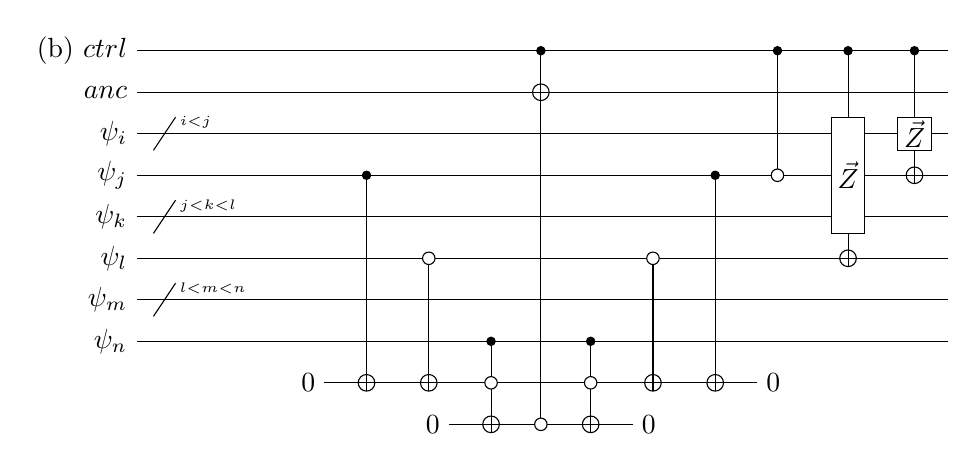
\begin{tikzpicture}[scale=1.000000,x=1pt,y=1pt]
\filldraw[color=white] (0.000000, -7.500000) rectangle (293.000000, 142.500000);
% Drawing wires
% Line 1: c W \text{(b) }ctrl
\draw[color=black] (0.000000,135.000000) -- (293.000000,135.000000);
\draw[color=black] (0.000000,135.000000) node[left] {$\text{(b) }ctrl$};
% Line 2: a W anc
\draw[color=black] (0.000000,120.000000) -- (293.000000,120.000000);
\draw[color=black] (0.000000,120.000000) node[left] {$anc$};
% Line 3: i W \psi_i
\draw[color=black] (0.000000,105.000000) -- (293.000000,105.000000);
\draw[color=black] (0.000000,105.000000) node[left] {$\psi_i$};
% Line 4: j W \psi_j
\draw[color=black] (0.000000,90.000000) -- (293.000000,90.000000);
\draw[color=black] (0.000000,90.000000) node[left] {$\psi_j$};
% Line 5: k W \psi_k
\draw[color=black] (0.000000,75.000000) -- (293.000000,75.000000);
\draw[color=black] (0.000000,75.000000) node[left] {$\psi_k$};
% Line 6: l W \psi_l
\draw[color=black] (0.000000,60.000000) -- (293.000000,60.000000);
\draw[color=black] (0.000000,60.000000) node[left] {$\psi_l$};
% Line 7: m W \psi_m
\draw[color=black] (0.000000,45.000000) -- (293.000000,45.000000);
\draw[color=black] (0.000000,45.000000) node[left] {$\psi_m$};
% Line 8: n W \psi_n
\draw[color=black] (0.000000,30.000000) -- (293.000000,30.000000);
\draw[color=black] (0.000000,30.000000) node[left] {$\psi_n$};
% Line 9: c0 W 0 0
\draw[color=black] (60.500000,15.000000) -- (231.500000,15.000000);
% Line 10: c1 W 0 0
\draw[color=black] (105.500000,0.000000) -- (186.500000,0.000000);
% Done with wires; drawing gates
% Line 12: i / ^{i<j}
\draw (6.000000, 99.000000) -- (14.000000, 111.000000);
\draw (12.000000, 108.000000) node[right] {$\scriptstyle{^{i<j}}$};
% Line 13: k / ^{j<k<l}
\draw (6.000000, 69.000000) -- (14.000000, 81.000000);
\draw (12.000000, 78.000000) node[right] {$\scriptstyle{^{j<k<l}}$};
% Line 14: m / ^{l<m<n}
\draw (6.000000, 39.000000) -- (14.000000, 51.000000);
\draw (12.000000, 48.000000) node[right] {$\scriptstyle{^{l<m<n}}$};
% Line 15: c a i j k l m n c0 c1 LABEL
% Line 16: c0 START
\draw[color=black] (68.000000,15.000000) node[fill=white,left,minimum height=15.000000pt,minimum width=15.000000pt,inner sep=0pt] {\phantom{$0$}};
\draw[color=black] (68.000000,15.000000) node[left] {$0$};
% Line 17: j +c0
\draw (83.000000,90.000000) -- (83.000000,15.000000);
\filldraw (83.000000, 90.000000) circle(1.500000pt);
\begin{scope}
\draw[fill=white] (83.000000, 15.000000) circle(3.000000pt);
\clip (83.000000, 15.000000) circle(3.000000pt);
\draw (80.000000, 15.000000) -- (86.000000, 15.000000);
\draw (83.000000, 12.000000) -- (83.000000, 18.000000);
\end{scope}
% Line 18: -l +c0
\draw (105.500000,60.000000) -- (105.500000,15.000000);
\draw[fill=white] (105.500000, 60.000000) circle(2.250000pt);
\begin{scope}
\draw[fill=white] (105.500000, 15.000000) circle(3.000000pt);
\clip (105.500000, 15.000000) circle(3.000000pt);
\draw (102.500000, 15.000000) -- (108.500000, 15.000000);
\draw (105.500000, 12.000000) -- (105.500000, 18.000000);
\end{scope}
% Line 19: c1 START
\draw[color=black] (113.000000,0.000000) node[fill=white,left,minimum height=15.000000pt,minimum width=15.000000pt,inner sep=0pt] {\phantom{$0$}};
\draw[color=black] (113.000000,0.000000) node[left] {$0$};
% Line 20: n -c0 +c1
\draw (128.000000,30.000000) -- (128.000000,0.000000);
\filldraw (128.000000, 30.000000) circle(1.500000pt);
\draw[fill=white] (128.000000, 15.000000) circle(2.250000pt);
\begin{scope}
\draw[fill=white] (128.000000, 0.000000) circle(3.000000pt);
\clip (128.000000, 0.000000) circle(3.000000pt);
\draw (125.000000, 0.000000) -- (131.000000, 0.000000);
\draw (128.000000, -3.000000) -- (128.000000, 3.000000);
\end{scope}
% Line 21: c -c1 +a
\draw (146.000000,135.000000) -- (146.000000,0.000000);
\filldraw (146.000000, 135.000000) circle(1.500000pt);
\draw[fill=white] (146.000000, 0.000000) circle(2.250000pt);
\begin{scope}
\draw[fill=white] (146.000000, 120.000000) circle(3.000000pt);
\clip (146.000000, 120.000000) circle(3.000000pt);
\draw (143.000000, 120.000000) -- (149.000000, 120.000000);
\draw (146.000000, 117.000000) -- (146.000000, 123.000000);
\end{scope}
% Line 22: n -c0 +c1
\draw (164.000000,30.000000) -- (164.000000,0.000000);
\filldraw (164.000000, 30.000000) circle(1.500000pt);
\draw[fill=white] (164.000000, 15.000000) circle(2.250000pt);
\begin{scope}
\draw[fill=white] (164.000000, 0.000000) circle(3.000000pt);
\clip (164.000000, 0.000000) circle(3.000000pt);
\draw (161.000000, 0.000000) -- (167.000000, 0.000000);
\draw (164.000000, -3.000000) -- (164.000000, 3.000000);
\end{scope}
% Line 23: c1 END
\draw[color=black] (179.000000,0.000000) node[fill=white,right,minimum height=15.000000pt,minimum width=15.000000pt,inner sep=0pt] {\phantom{$0$}};
\draw[color=black] (179.000000,0.000000) node[right] {$0$};
% Line 24: -l +c0
\draw (186.500000,60.000000) -- (186.500000,15.000000);
\draw[fill=white] (186.500000, 60.000000) circle(2.250000pt);
\begin{scope}
\draw[fill=white] (186.500000, 15.000000) circle(3.000000pt);
\clip (186.500000, 15.000000) circle(3.000000pt);
\draw (183.500000, 15.000000) -- (189.500000, 15.000000);
\draw (186.500000, 12.000000) -- (186.500000, 18.000000);
\end{scope}
% Line 25: j +c0
\draw (209.000000,90.000000) -- (209.000000,15.000000);
\filldraw (209.000000, 90.000000) circle(1.500000pt);
\begin{scope}
\draw[fill=white] (209.000000, 15.000000) circle(3.000000pt);
\clip (209.000000, 15.000000) circle(3.000000pt);
\draw (206.000000, 15.000000) -- (212.000000, 15.000000);
\draw (209.000000, 12.000000) -- (209.000000, 18.000000);
\end{scope}
% Line 26: c0 END
\draw[color=black] (224.000000,15.000000) node[fill=white,right,minimum height=15.000000pt,minimum width=15.000000pt,inner sep=0pt] {\phantom{$0$}};
\draw[color=black] (224.000000,15.000000) node[right] {$0$};
% Line 27: c -j
\draw (231.500000,135.000000) -- (231.500000,90.000000);
\filldraw (231.500000, 135.000000) circle(1.500000pt);
\draw[fill=white] (231.500000, 90.000000) circle(2.250000pt);
% Line 29: i j k G $\vec{Z}$ c +l
\draw (257.000000,135.000000) -- (257.000000,60.000000);
\begin{scope}
\draw[fill=white] (257.000000, 90.000000) +(-45.000000:8.485281pt and 29.698485pt) -- +(45.000000:8.485281pt and 29.698485pt) -- +(135.000000:8.485281pt and 29.698485pt) -- +(225.000000:8.485281pt and 29.698485pt) -- cycle;
\clip (257.000000, 90.000000) +(-45.000000:8.485281pt and 29.698485pt) -- +(45.000000:8.485281pt and 29.698485pt) -- +(135.000000:8.485281pt and 29.698485pt) -- +(225.000000:8.485281pt and 29.698485pt) -- cycle;
\draw (257.000000, 90.000000) node {$\vec{Z}$};
\end{scope}
\filldraw (257.000000, 135.000000) circle(1.500000pt);
\begin{scope}
\draw[fill=white] (257.000000, 60.000000) circle(3.000000pt);
\clip (257.000000, 60.000000) circle(3.000000pt);
\draw (254.000000, 60.000000) -- (260.000000, 60.000000);
\draw (257.000000, 57.000000) -- (257.000000, 63.000000);
\end{scope}
% Line 30: i G $\vec{Z}$ c +j
\draw (281.000000,135.000000) -- (281.000000,90.000000);
\begin{scope}
\draw[fill=white] (281.000000, 105.000000) +(-45.000000:8.485281pt and 8.485281pt) -- +(45.000000:8.485281pt and 8.485281pt) -- +(135.000000:8.485281pt and 8.485281pt) -- +(225.000000:8.485281pt and 8.485281pt) -- cycle;
\clip (281.000000, 105.000000) +(-45.000000:8.485281pt and 8.485281pt) -- +(45.000000:8.485281pt and 8.485281pt) -- +(135.000000:8.485281pt and 8.485281pt) -- +(225.000000:8.485281pt and 8.485281pt) -- cycle;
\draw (281.000000, 105.000000) node {$\vec{Z}$};
\end{scope}
\filldraw (281.000000, 135.000000) circle(1.500000pt);
\begin{scope}
\draw[fill=white] (281.000000, 90.000000) circle(3.000000pt);
\clip (281.000000, 90.000000) circle(3.000000pt);
\draw (278.000000, 90.000000) -- (284.000000, 90.000000);
\draw (281.000000, 87.000000) -- (281.000000, 93.000000);
\end{scope}
% Done with gates; drawing ending labels
% Done with ending labels; drawing cut lines and comments
% Done with comments
\end{tikzpicture}

    \caption{
        \textbf{Block-Encoding Product of Fermionic Operators Plus Hermitian Conjugate (modifications)}
        In subfigure (a), a block-encoding for the operator $b_j b_l^\dagger + b_l b_j^\dagger$ is given.
        In subfigure (b), a block-encoding for the operator $b_j b_l^\dagger b_n^\dagger b_n + b_n^\dagger b_n b_l b_j^\dagger$ is given.
    }
    \label{fig:fermionic-be-lc-modifications}
\end{figure}

For an operator of the form $b_j b_l^\dagger + b_l b_j^\dagger$, we can construct a similar block-encoding with a slight modification.
In this case, we simply flip the occupation of the $l^\text{th}$ mode using a Pauli $X$ gate before we compute the parity of the modes.
The circuit diagram for block-encoding this operator is given in subfigure \ref{fig:fermionic-be-lc-modifications}a.

Likewise, if a number operator is included in a term, this can be accounted for by including a $1$-control on that mode when determining if the block-encoding ancilla should be flipped and excluding that mode from any parity computations.
An example circuit diagram for an operator including a number operator is given in subfigure \ref{fig:fermionic-be-lc-modifications}b.

\begin{figure}
    \definecolor{tblue}{RGB}{61,142,221}
\definecolor{torange}{RGB}{253,143,41}
\begin{tikzpicture}[scale=1.000000,x=1pt,y=1pt]
\filldraw[color=white] (0.000000, -7.500000) rectangle (477.000000, 157.500000);
% Drawing wires
% Line 4: ctrl W ctrl
\draw[color=black] (0.000000,150.000000) -- (477.000000,150.000000);
\draw[color=black] (0.000000,150.000000) node[left] {$ctrl$};
% Line 5: anc W anc
\draw[color=black] (0.000000,135.000000) -- (477.000000,135.000000);
\draw[color=black] (0.000000,135.000000) node[left] {$anc$};
% Line 6: a W \psi_i
\draw[color=black] (0.000000,120.000000) -- (477.000000,120.000000);
\draw[color=black] (0.000000,120.000000) node[left] {$\psi_i$};
% Line 7: b W \psi_j
\draw[color=black] (0.000000,105.000000) -- (477.000000,105.000000);
\draw[color=black] (0.000000,105.000000) node[left] {$\psi_j$};
% Line 8: c W \vdots
\draw[color=black] (0.000000,90.000000) -- (477.000000,90.000000);
\draw[color=black] (0.000000,90.000000) node[left] {$\vdots$};
% Line 9: f W \psi_m
\draw[color=black] (0.000000,75.000000) -- (477.000000,75.000000);
\draw[color=black] (0.000000,75.000000) node[left] {$\psi_m$};
% Line 10: c0 W 0 0
\draw[color=black] (13.500000,60.000000) -- (346.500000,60.000000);
% Line 11: c1 W 0 0
\draw[color=black] (40.500000,45.000000) -- (319.500000,45.000000);
% Line 12: c2 W 0 0
\draw[color=black] (67.500000,30.000000) -- (292.500000,30.000000);
% Line 13: 1 W 0 0
\draw[color=black] (94.500000,15.000000) -- (265.500000,15.000000);
% Line 14: c3 W 0 0
\draw[color=black] (139.500000,0.000000) -- (220.500000,0.000000);
% Done with wires; drawing gates
% Line 16: c0 START
\draw[color=black] (21.000000,60.000000) node[fill=white,left,minimum height=15.000000pt,minimum width=15.000000pt,inner sep=0pt] {\phantom{$0$}};
\draw[color=black] (21.000000,60.000000) node[left] {$0$};
% Line 17: a +c0
\draw (40.500000,120.000000) -- (40.500000,60.000000);
\filldraw (40.500000, 120.000000) circle(1.500000pt);
\begin{scope}
\draw[fill=white] (40.500000, 60.000000) circle(3.000000pt);
\clip (40.500000, 60.000000) circle(3.000000pt);
\draw (37.500000, 60.000000) -- (43.500000, 60.000000);
\draw (40.500000, 57.000000) -- (40.500000, 63.000000);
\end{scope}
% Line 18: c1 START
\draw[color=black] (48.000000,45.000000) node[fill=white,left,minimum height=15.000000pt,minimum width=15.000000pt,inner sep=0pt] {\phantom{$0$}};
\draw[color=black] (48.000000,45.000000) node[left] {$0$};
% Line 19: b +c0 +c1
\draw (67.500000,105.000000) -- (67.500000,45.000000);
\filldraw (67.500000, 105.000000) circle(1.500000pt);
\begin{scope}
\draw[fill=white] (67.500000, 60.000000) circle(3.000000pt);
\clip (67.500000, 60.000000) circle(3.000000pt);
\draw (64.500000, 60.000000) -- (70.500000, 60.000000);
\draw (67.500000, 57.000000) -- (67.500000, 63.000000);
\end{scope}
\begin{scope}
\draw[fill=white] (67.500000, 45.000000) circle(3.000000pt);
\clip (67.500000, 45.000000) circle(3.000000pt);
\draw (64.500000, 45.000000) -- (70.500000, 45.000000);
\draw (67.500000, 42.000000) -- (67.500000, 48.000000);
\end{scope}
% Line 20: c2 START
\draw[color=black] (75.000000,30.000000) node[fill=white,left,minimum height=15.000000pt,minimum width=15.000000pt,inner sep=0pt] {\phantom{$0$}};
\draw[color=black] (75.000000,30.000000) node[left] {$0$};
% Line 21: c +c1 +c2
\draw (94.500000,90.000000) -- (94.500000,30.000000);
\filldraw (94.500000, 90.000000) circle(1.500000pt);
\begin{scope}
\draw[fill=white] (94.500000, 45.000000) circle(3.000000pt);
\clip (94.500000, 45.000000) circle(3.000000pt);
\draw (91.500000, 45.000000) -- (97.500000, 45.000000);
\draw (94.500000, 42.000000) -- (94.500000, 48.000000);
\end{scope}
\begin{scope}
\draw[fill=white] (94.500000, 30.000000) circle(3.000000pt);
\clip (94.500000, 30.000000) circle(3.000000pt);
\draw (91.500000, 30.000000) -- (97.500000, 30.000000);
\draw (94.500000, 27.000000) -- (94.500000, 33.000000);
\end{scope}
% Line 22: 1 START
\draw[color=black] (102.000000,15.000000) node[fill=white,left,minimum height=15.000000pt,minimum width=15.000000pt,inner sep=0pt] {\phantom{$0$}};
\draw[color=black] (102.000000,15.000000) node[left] {$0$};
% Line 23: c +1
\draw (117.000000,90.000000) -- (117.000000,15.000000);
\filldraw (117.000000, 90.000000) circle(1.500000pt);
\begin{scope}
\draw[fill=white] (117.000000, 15.000000) circle(3.000000pt);
\clip (117.000000, 15.000000) circle(3.000000pt);
\draw (114.000000, 15.000000) -- (120.000000, 15.000000);
\draw (117.000000, 12.000000) -- (117.000000, 18.000000);
\end{scope}
% Line 24: f +1
\draw (139.500000,75.000000) -- (139.500000,15.000000);
\filldraw (139.500000, 75.000000) circle(1.500000pt);
\begin{scope}
\draw[fill=white] (139.500000, 15.000000) circle(3.000000pt);
\clip (139.500000, 15.000000) circle(3.000000pt);
\draw (136.500000, 15.000000) -- (142.500000, 15.000000);
\draw (139.500000, 12.000000) -- (139.500000, 18.000000);
\end{scope}
% Line 26: c3 START
\draw[color=black] (147.000000,0.000000) node[fill=white,left,minimum height=15.000000pt,minimum width=15.000000pt,inner sep=0pt] {\phantom{$0$}};
\draw[color=black] (147.000000,0.000000) node[left] {$0$};
% Line 27: -c0 -c1 -c2 -1 +c3
\draw (162.000000,60.000000) -- (162.000000,0.000000);
\draw[fill=white] (162.000000, 60.000000) circle(2.250000pt);
\draw[fill=white] (162.000000, 45.000000) circle(2.250000pt);
\draw[fill=white] (162.000000, 30.000000) circle(2.250000pt);
\draw[fill=white] (162.000000, 15.000000) circle(2.250000pt);
\begin{scope}
\draw[fill=white] (162.000000, 0.000000) circle(3.000000pt);
\clip (162.000000, 0.000000) circle(3.000000pt);
\draw (159.000000, 0.000000) -- (165.000000, 0.000000);
\draw (162.000000, -3.000000) -- (162.000000, 3.000000);
\end{scope}
% Line 28: ctrl -c3 +anc
\draw (180.000000,150.000000) -- (180.000000,0.000000);
\filldraw (180.000000, 150.000000) circle(1.500000pt);
\draw[fill=white] (180.000000, 0.000000) circle(2.250000pt);
\begin{scope}
\draw[fill=white] (180.000000, 135.000000) circle(3.000000pt);
\clip (180.000000, 135.000000) circle(3.000000pt);
\draw (177.000000, 135.000000) -- (183.000000, 135.000000);
\draw (180.000000, 132.000000) -- (180.000000, 138.000000);
\end{scope}
% Line 29: -c0 -c1 -c2 -1 +c3
\draw (198.000000,60.000000) -- (198.000000,0.000000);
\draw[fill=white] (198.000000, 60.000000) circle(2.250000pt);
\draw[fill=white] (198.000000, 45.000000) circle(2.250000pt);
\draw[fill=white] (198.000000, 30.000000) circle(2.250000pt);
\draw[fill=white] (198.000000, 15.000000) circle(2.250000pt);
\begin{scope}
\draw[fill=white] (198.000000, 0.000000) circle(3.000000pt);
\clip (198.000000, 0.000000) circle(3.000000pt);
\draw (195.000000, 0.000000) -- (201.000000, 0.000000);
\draw (198.000000, -3.000000) -- (198.000000, 3.000000);
\end{scope}
% Line 30: c3 END
\draw[color=black] (213.000000,0.000000) node[fill=white,right,minimum height=15.000000pt,minimum width=15.000000pt,inner sep=0pt] {\phantom{$0$}};
\draw[color=black] (213.000000,0.000000) node[right] {$0$};
% Line 32: f +1
\draw (220.500000,75.000000) -- (220.500000,15.000000);
\filldraw (220.500000, 75.000000) circle(1.500000pt);
\begin{scope}
\draw[fill=white] (220.500000, 15.000000) circle(3.000000pt);
\clip (220.500000, 15.000000) circle(3.000000pt);
\draw (217.500000, 15.000000) -- (223.500000, 15.000000);
\draw (220.500000, 12.000000) -- (220.500000, 18.000000);
\end{scope}
% Line 33: c +1
\draw (243.000000,90.000000) -- (243.000000,15.000000);
\filldraw (243.000000, 90.000000) circle(1.500000pt);
\begin{scope}
\draw[fill=white] (243.000000, 15.000000) circle(3.000000pt);
\clip (243.000000, 15.000000) circle(3.000000pt);
\draw (240.000000, 15.000000) -- (246.000000, 15.000000);
\draw (243.000000, 12.000000) -- (243.000000, 18.000000);
\end{scope}
% Line 34: 1 END
\draw[color=black] (258.000000,15.000000) node[fill=white,right,minimum height=15.000000pt,minimum width=15.000000pt,inner sep=0pt] {\phantom{$0$}};
\draw[color=black] (258.000000,15.000000) node[right] {$0$};
% Line 35: c +c1 +c2
\draw (265.500000,90.000000) -- (265.500000,30.000000);
\filldraw (265.500000, 90.000000) circle(1.500000pt);
\begin{scope}
\draw[fill=white] (265.500000, 45.000000) circle(3.000000pt);
\clip (265.500000, 45.000000) circle(3.000000pt);
\draw (262.500000, 45.000000) -- (268.500000, 45.000000);
\draw (265.500000, 42.000000) -- (265.500000, 48.000000);
\end{scope}
\begin{scope}
\draw[fill=white] (265.500000, 30.000000) circle(3.000000pt);
\clip (265.500000, 30.000000) circle(3.000000pt);
\draw (262.500000, 30.000000) -- (268.500000, 30.000000);
\draw (265.500000, 27.000000) -- (265.500000, 33.000000);
\end{scope}
% Line 36: c2 END
\draw[color=black] (285.000000,30.000000) node[fill=white,right,minimum height=15.000000pt,minimum width=15.000000pt,inner sep=0pt] {\phantom{$0$}};
\draw[color=black] (285.000000,30.000000) node[right] {$0$};
% Line 37: b +c0 +c1
\draw (292.500000,105.000000) -- (292.500000,45.000000);
\filldraw (292.500000, 105.000000) circle(1.500000pt);
\begin{scope}
\draw[fill=white] (292.500000, 60.000000) circle(3.000000pt);
\clip (292.500000, 60.000000) circle(3.000000pt);
\draw (289.500000, 60.000000) -- (295.500000, 60.000000);
\draw (292.500000, 57.000000) -- (292.500000, 63.000000);
\end{scope}
\begin{scope}
\draw[fill=white] (292.500000, 45.000000) circle(3.000000pt);
\clip (292.500000, 45.000000) circle(3.000000pt);
\draw (289.500000, 45.000000) -- (295.500000, 45.000000);
\draw (292.500000, 42.000000) -- (292.500000, 48.000000);
\end{scope}
% Line 38: c1 END
\draw[color=black] (312.000000,45.000000) node[fill=white,right,minimum height=15.000000pt,minimum width=15.000000pt,inner sep=0pt] {\phantom{$0$}};
\draw[color=black] (312.000000,45.000000) node[right] {$0$};
% Line 39: a +c0
\draw (319.500000,120.000000) -- (319.500000,60.000000);
\filldraw (319.500000, 120.000000) circle(1.500000pt);
\begin{scope}
\draw[fill=white] (319.500000, 60.000000) circle(3.000000pt);
\clip (319.500000, 60.000000) circle(3.000000pt);
\draw (316.500000, 60.000000) -- (322.500000, 60.000000);
\draw (319.500000, 57.000000) -- (319.500000, 63.000000);
\end{scope}
% Line 40: c0 END
\draw[color=black] (339.000000,60.000000) node[fill=white,right,minimum height=15.000000pt,minimum width=15.000000pt,inner sep=0pt] {\phantom{$0$}};
\draw[color=black] (339.000000,60.000000) node[right] {$0$};
% Line 44: ctrl -a color=torange
\begin{scope}[color=torange]
\draw (346.500000,150.000000) -- (346.500000,120.000000);
\filldraw (346.500000, 150.000000) circle(1.500000pt);
\draw[fill=white] (346.500000, 120.000000) circle(2.250000pt);
\end{scope}
% Line 46: a b c G $\vec{Z}$ ctrl +f
\draw (372.000000,150.000000) -- (372.000000,75.000000);
\begin{scope}
\draw[fill=white] (372.000000, 105.000000) +(-45.000000:8.485281pt and 29.698485pt) -- +(45.000000:8.485281pt and 29.698485pt) -- +(135.000000:8.485281pt and 29.698485pt) -- +(225.000000:8.485281pt and 29.698485pt) -- cycle;
\clip (372.000000, 105.000000) +(-45.000000:8.485281pt and 29.698485pt) -- +(45.000000:8.485281pt and 29.698485pt) -- +(135.000000:8.485281pt and 29.698485pt) -- +(225.000000:8.485281pt and 29.698485pt) -- cycle;
\draw (372.000000, 105.000000) node {$\vec{Z}$};
\end{scope}
\filldraw (372.000000, 150.000000) circle(1.500000pt);
\begin{scope}
\draw[fill=white] (372.000000, 75.000000) circle(3.000000pt);
\clip (372.000000, 75.000000) circle(3.000000pt);
\draw (369.000000, 75.000000) -- (375.000000, 75.000000);
\draw (372.000000, 72.000000) -- (372.000000, 78.000000);
\end{scope}
% Line 47: ctrl a b c LABEL ...
\draw[color=black] (397.500000, 150.000000) node [fill=white] {$\cdots$};
\draw[color=black] (397.500000, 120.000000) node [fill=white] {$\cdots$};
\draw[color=black] (397.500000, 105.000000) node [fill=white] {$\cdots$};
\draw[color=black] (397.500000, 90.000000) node [fill=white] {$\cdots$};
% Line 48: a b G $\vec{Z}$ ctrl +c
\draw (423.000000,150.000000) -- (423.000000,90.000000);
\begin{scope}
\draw[fill=white] (423.000000, 112.500000) +(-45.000000:8.485281pt and 19.091883pt) -- +(45.000000:8.485281pt and 19.091883pt) -- +(135.000000:8.485281pt and 19.091883pt) -- +(225.000000:8.485281pt and 19.091883pt) -- cycle;
\clip (423.000000, 112.500000) +(-45.000000:8.485281pt and 19.091883pt) -- +(45.000000:8.485281pt and 19.091883pt) -- +(135.000000:8.485281pt and 19.091883pt) -- +(225.000000:8.485281pt and 19.091883pt) -- cycle;
\draw (423.000000, 112.500000) node {$\vec{Z}$};
\end{scope}
\filldraw (423.000000, 150.000000) circle(1.500000pt);
\begin{scope}
\draw[fill=white] (423.000000, 90.000000) circle(3.000000pt);
\clip (423.000000, 90.000000) circle(3.000000pt);
\draw (420.000000, 90.000000) -- (426.000000, 90.000000);
\draw (423.000000, 87.000000) -- (423.000000, 93.000000);
\end{scope}
% Line 49: a G $\vec{Z}$ ctrl +b
\draw (447.000000,150.000000) -- (447.000000,105.000000);
\begin{scope}
\draw[fill=white] (447.000000, 120.000000) +(-45.000000:8.485281pt and 8.485281pt) -- +(45.000000:8.485281pt and 8.485281pt) -- +(135.000000:8.485281pt and 8.485281pt) -- +(225.000000:8.485281pt and 8.485281pt) -- cycle;
\clip (447.000000, 120.000000) +(-45.000000:8.485281pt and 8.485281pt) -- +(45.000000:8.485281pt and 8.485281pt) -- +(135.000000:8.485281pt and 8.485281pt) -- +(225.000000:8.485281pt and 8.485281pt) -- cycle;
\draw (447.000000, 120.000000) node {$\vec{Z}$};
\end{scope}
\filldraw (447.000000, 150.000000) circle(1.500000pt);
\begin{scope}
\draw[fill=white] (447.000000, 105.000000) circle(3.000000pt);
\clip (447.000000, 105.000000) circle(3.000000pt);
\draw (444.000000, 105.000000) -- (450.000000, 105.000000);
\draw (447.000000, 102.000000) -- (447.000000, 108.000000);
\end{scope}
% Line 50: ctrl +a
\draw (468.000000,150.000000) -- (468.000000,120.000000);
\filldraw (468.000000, 150.000000) circle(1.500000pt);
\begin{scope}
\draw[fill=white] (468.000000, 120.000000) circle(3.000000pt);
\clip (468.000000, 120.000000) circle(3.000000pt);
\draw (465.000000, 120.000000) -- (471.000000, 120.000000);
\draw (468.000000, 117.000000) -- (468.000000, 123.000000);
\end{scope}
% Done with gates; drawing ending labels
% Done with ending labels; drawing cut lines and comments
% Done with comments
\end{tikzpicture}

    \caption{
        \textbf{Generalized Block-Encoding for Product of Fermionic Operators Plus Hermitian Conjugate}
        A block-encoding for the operator $b_i b_j ... b_m + b_m^\dagger ... b_j^\dagger b_i^\dagger$ is given.
        The $CZ$ gate highlighted in orange is present only if the swapping on the order of the operators in the second term induces a negative sign (an odd number of swaps are required).
        Block-encodings for similar operators such as those that include number operators or different arrangements of the creation and annihilation operators can be accounted for using the modifications shown in Figure \ref{fig:fermionic-be-lc-modifications}.
    }
    \label{fig:fermionic-be-lc}
\end{figure}

The construction of these block-encoding circuits can be generalized to any operator that is a product of fermionic operators plus its hermitian conjugate.
An example circuit diagram for this generalized construction is shown in Figure \ref{fig:fermionic-be-lc}.
If $C$ represents the number of active modes excluding modes where a number operator is acting on the mode, then the $CZ$ gate is present only if $(C \text{ choose } 2)$ is odd.
These block-encoding circuits will all have optimal rescaling factors ($\lambda=1$), require one block-encoding ancilla and $B - 1$ clean ancillae, and use $4(B-1)$ T gates.

\begin{figure}
    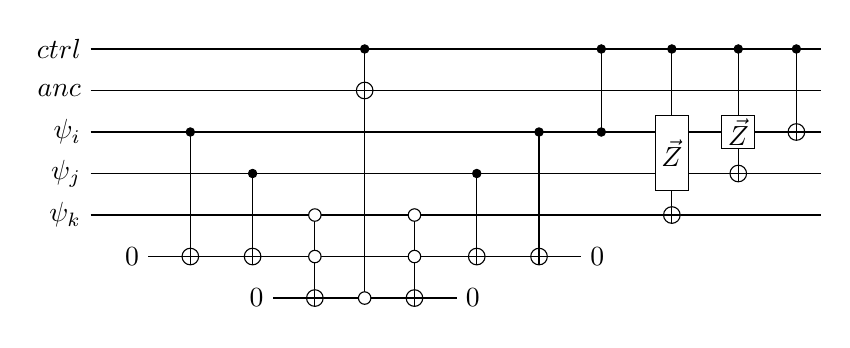
\begin{tikzpicture}[scale=1.000000,x=1pt,y=1pt]
\filldraw[color=white] (0.000000, -7.500000) rectangle (264.000000, 97.500000);
% Drawing wires
% Line 1: ctrl W ctrl
\draw[color=black] (0.000000,90.000000) -- (264.000000,90.000000);
\draw[color=black] (0.000000,90.000000) node[left] {$ctrl$};
% Line 2: anc W anc
\draw[color=black] (0.000000,75.000000) -- (264.000000,75.000000);
\draw[color=black] (0.000000,75.000000) node[left] {$anc$};
% Line 3: i W \psi_i
\draw[color=black] (0.000000,60.000000) -- (264.000000,60.000000);
\draw[color=black] (0.000000,60.000000) node[left] {$\psi_i$};
% Line 4: j W \psi_j
\draw[color=black] (0.000000,45.000000) -- (264.000000,45.000000);
\draw[color=black] (0.000000,45.000000) node[left] {$\psi_j$};
% Line 5: k W \psi_k
\draw[color=black] (0.000000,30.000000) -- (264.000000,30.000000);
\draw[color=black] (0.000000,30.000000) node[left] {$\psi_k$};
% Line 6: c0 W 0 0
\draw[color=black] (13.500000,15.000000) -- (184.500000,15.000000);
% Line 7: c1 W 0 0
\draw[color=black] (58.500000,0.000000) -- (139.500000,0.000000);
% Done with wires; drawing gates
% Line 9: c0 START
\draw[color=black] (21.000000,15.000000) node[fill=white,left,minimum height=15.000000pt,minimum width=15.000000pt,inner sep=0pt] {\phantom{$0$}};
\draw[color=black] (21.000000,15.000000) node[left] {$0$};
% Line 10: i +c0
\draw (36.000000,60.000000) -- (36.000000,15.000000);
\filldraw (36.000000, 60.000000) circle(1.500000pt);
\begin{scope}
\draw[fill=white] (36.000000, 15.000000) circle(3.000000pt);
\clip (36.000000, 15.000000) circle(3.000000pt);
\draw (33.000000, 15.000000) -- (39.000000, 15.000000);
\draw (36.000000, 12.000000) -- (36.000000, 18.000000);
\end{scope}
% Line 11: j +c0
\draw (58.500000,45.000000) -- (58.500000,15.000000);
\filldraw (58.500000, 45.000000) circle(1.500000pt);
\begin{scope}
\draw[fill=white] (58.500000, 15.000000) circle(3.000000pt);
\clip (58.500000, 15.000000) circle(3.000000pt);
\draw (55.500000, 15.000000) -- (61.500000, 15.000000);
\draw (58.500000, 12.000000) -- (58.500000, 18.000000);
\end{scope}
% Line 12: c1 START
\draw[color=black] (66.000000,0.000000) node[fill=white,left,minimum height=15.000000pt,minimum width=15.000000pt,inner sep=0pt] {\phantom{$0$}};
\draw[color=black] (66.000000,0.000000) node[left] {$0$};
% Line 13: -k -c0 +c1
\draw (81.000000,30.000000) -- (81.000000,0.000000);
\draw[fill=white] (81.000000, 30.000000) circle(2.250000pt);
\draw[fill=white] (81.000000, 15.000000) circle(2.250000pt);
\begin{scope}
\draw[fill=white] (81.000000, 0.000000) circle(3.000000pt);
\clip (81.000000, 0.000000) circle(3.000000pt);
\draw (78.000000, 0.000000) -- (84.000000, 0.000000);
\draw (81.000000, -3.000000) -- (81.000000, 3.000000);
\end{scope}
% Line 14: ctrl -c1 +anc
\draw (99.000000,90.000000) -- (99.000000,0.000000);
\filldraw (99.000000, 90.000000) circle(1.500000pt);
\draw[fill=white] (99.000000, 0.000000) circle(2.250000pt);
\begin{scope}
\draw[fill=white] (99.000000, 75.000000) circle(3.000000pt);
\clip (99.000000, 75.000000) circle(3.000000pt);
\draw (96.000000, 75.000000) -- (102.000000, 75.000000);
\draw (99.000000, 72.000000) -- (99.000000, 78.000000);
\end{scope}
% Line 15: -k -c0 +c1
\draw (117.000000,30.000000) -- (117.000000,0.000000);
\draw[fill=white] (117.000000, 30.000000) circle(2.250000pt);
\draw[fill=white] (117.000000, 15.000000) circle(2.250000pt);
\begin{scope}
\draw[fill=white] (117.000000, 0.000000) circle(3.000000pt);
\clip (117.000000, 0.000000) circle(3.000000pt);
\draw (114.000000, 0.000000) -- (120.000000, 0.000000);
\draw (117.000000, -3.000000) -- (117.000000, 3.000000);
\end{scope}
% Line 16: c1 END
\draw[color=black] (132.000000,0.000000) node[fill=white,right,minimum height=15.000000pt,minimum width=15.000000pt,inner sep=0pt] {\phantom{$0$}};
\draw[color=black] (132.000000,0.000000) node[right] {$0$};
% Line 17: j +c0
\draw (139.500000,45.000000) -- (139.500000,15.000000);
\filldraw (139.500000, 45.000000) circle(1.500000pt);
\begin{scope}
\draw[fill=white] (139.500000, 15.000000) circle(3.000000pt);
\clip (139.500000, 15.000000) circle(3.000000pt);
\draw (136.500000, 15.000000) -- (142.500000, 15.000000);
\draw (139.500000, 12.000000) -- (139.500000, 18.000000);
\end{scope}
% Line 18: i +c0
\draw (162.000000,60.000000) -- (162.000000,15.000000);
\filldraw (162.000000, 60.000000) circle(1.500000pt);
\begin{scope}
\draw[fill=white] (162.000000, 15.000000) circle(3.000000pt);
\clip (162.000000, 15.000000) circle(3.000000pt);
\draw (159.000000, 15.000000) -- (165.000000, 15.000000);
\draw (162.000000, 12.000000) -- (162.000000, 18.000000);
\end{scope}
% Line 19: c0 END
\draw[color=black] (177.000000,15.000000) node[fill=white,right,minimum height=15.000000pt,minimum width=15.000000pt,inner sep=0pt] {\phantom{$0$}};
\draw[color=black] (177.000000,15.000000) node[right] {$0$};
% Line 21: ctrl i
\draw (184.500000,90.000000) -- (184.500000,60.000000);
\filldraw (184.500000, 90.000000) circle(1.500000pt);
\filldraw (184.500000, 60.000000) circle(1.500000pt);
% Line 23: i j G $\vec{Z}$ ctrl +k
\draw (210.000000,90.000000) -- (210.000000,30.000000);
\begin{scope}
\draw[fill=white] (210.000000, 52.500000) +(-45.000000:8.485281pt and 19.091883pt) -- +(45.000000:8.485281pt and 19.091883pt) -- +(135.000000:8.485281pt and 19.091883pt) -- +(225.000000:8.485281pt and 19.091883pt) -- cycle;
\clip (210.000000, 52.500000) +(-45.000000:8.485281pt and 19.091883pt) -- +(45.000000:8.485281pt and 19.091883pt) -- +(135.000000:8.485281pt and 19.091883pt) -- +(225.000000:8.485281pt and 19.091883pt) -- cycle;
\draw (210.000000, 52.500000) node {$\vec{Z}$};
\end{scope}
\filldraw (210.000000, 90.000000) circle(1.500000pt);
\begin{scope}
\draw[fill=white] (210.000000, 30.000000) circle(3.000000pt);
\clip (210.000000, 30.000000) circle(3.000000pt);
\draw (207.000000, 30.000000) -- (213.000000, 30.000000);
\draw (210.000000, 27.000000) -- (210.000000, 33.000000);
\end{scope}
% Line 24: i G $\vec{Z}$ ctrl +j
\draw (234.000000,90.000000) -- (234.000000,45.000000);
\begin{scope}
\draw[fill=white] (234.000000, 60.000000) +(-45.000000:8.485281pt and 8.485281pt) -- +(45.000000:8.485281pt and 8.485281pt) -- +(135.000000:8.485281pt and 8.485281pt) -- +(225.000000:8.485281pt and 8.485281pt) -- cycle;
\clip (234.000000, 60.000000) +(-45.000000:8.485281pt and 8.485281pt) -- +(45.000000:8.485281pt and 8.485281pt) -- +(135.000000:8.485281pt and 8.485281pt) -- +(225.000000:8.485281pt and 8.485281pt) -- cycle;
\draw (234.000000, 60.000000) node {$\vec{Z}$};
\end{scope}
\filldraw (234.000000, 90.000000) circle(1.500000pt);
\begin{scope}
\draw[fill=white] (234.000000, 45.000000) circle(3.000000pt);
\clip (234.000000, 45.000000) circle(3.000000pt);
\draw (231.000000, 45.000000) -- (237.000000, 45.000000);
\draw (234.000000, 42.000000) -- (234.000000, 48.000000);
\end{scope}
% Line 25: ctrl +i
\draw (255.000000,90.000000) -- (255.000000,60.000000);
\filldraw (255.000000, 90.000000) circle(1.500000pt);
\begin{scope}
\draw[fill=white] (255.000000, 60.000000) circle(3.000000pt);
\clip (255.000000, 60.000000) circle(3.000000pt);
\draw (252.000000, 60.000000) -- (258.000000, 60.000000);
\draw (255.000000, 57.000000) -- (255.000000, 63.000000);
\end{scope}
% Done with gates; drawing ending labels
% Done with ending labels; drawing cut lines and comments
% Done with comments
\end{tikzpicture}

    \caption{
        \textbf{Block-Encoding for Linear Combination of Non-Conjugate Fermionic Operators}
        A block-encoding for the operator $b_i b_j b_k^\dagger + b_j^\dagger b_i^\dagger b_k^\dagger$ is given.
    }
    \label{fig:fermionic-be-lc-not-conjugate}
\end{figure}

As mentioned, the strategy employed here to construct block-encodings of a linear combination of fermionic ladder operators is not restricted to hermitian conjugates.
Consider the action of the operator $b_i b_j b_k^\dagger + b_j^\dagger b_i^\dagger b_k^\dagger$ on the occupation states of the fermionic modes.
This operator will zero-out the state \textit{unless} both $\ket{\psi_{b_i}} \oplus \ket{\psi_{b_j}}$ and $\ket{\psi_{b_k}}$ are $\ket{0}$.
The implementation of the block-encoding for this operator is given in Figure \ref{fig:fermionic-be-lc-not-conjugate}.
This block-encoding circuit has an optimal rescaling factor ($\lambda = 1$), requires one block-encoding ancilla and two clean ancillae, and uses $8$ T gates.

\subsection{Bosonic Ladder Operators}

In this section, we aim to define a family of unitaries that generate block-encodings of the bosonic creation ($a_i^\dagger$) and annihilation ($a_i$) operators.
From the defined action of the bosonic creation operator (Equation \ref{eq:bosonic-creation}), it is clear that we can define a block-encoding unitary of the form of Eq. \ref{eq:general-block-encoding}: 
\begin{equation}
    \label{eq:be-bos-creation}
    U_{a^\dagger_i} \ket{\omega_i} \ket{0}_\text{anc} = 
    \begin{cases}
        \sqrt{\omega_i + 1 / \Omega} \ket{\omega_i + 1} \ket{0}_\text{anc} + \beta_\psi \ket{\perp} & \text{when } \omega_i < \Omega \\
        \ket{\perp} & \text{when } \omega_i = \Omega \\
    
    \end{cases}
\end{equation}
where $\omega_i$ is the occupation number of the $i^\text{th}$ bosonic mode and the operator is rescaled by a factor of $\sqrt{\Omega}$.

\begin{figure}
    \mbox{
        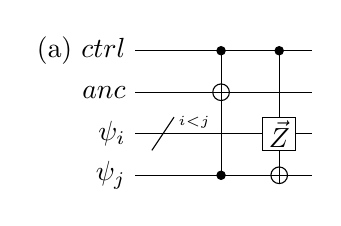
\begin{tikzpicture}[scale=1.000000,x=1pt,y=1pt]
\filldraw[color=white] (0.000000, -7.500000) rectangle (64.000000, 52.500000);
% Drawing wires
% Line 1: ctrl W \text{(a) }ctrl
\draw[color=black] (0.000000,45.000000) -- (64.000000,45.000000);
\draw[color=black] (0.000000,45.000000) node[left] {$\text{(a) }ctrl$};
% Line 2: anc W anc
\draw[color=black] (0.000000,30.000000) -- (64.000000,30.000000);
\draw[color=black] (0.000000,30.000000) node[left] {$anc$};
% Line 3: i W \psi_i
\draw[color=black] (0.000000,15.000000) -- (64.000000,15.000000);
\draw[color=black] (0.000000,15.000000) node[left] {$\psi_i$};
% Line 4: j W \psi_j
\draw[color=black] (0.000000,0.000000) -- (64.000000,0.000000);
\draw[color=black] (0.000000,0.000000) node[left] {$\psi_j$};
% Done with wires; drawing gates
% Line 6: i / ^{i<j}
\draw (6.000000, 9.000000) -- (14.000000, 21.000000);
\draw (12.000000, 18.000000) node[right] {$\scriptstyle{^{i<j}}$};
% Line 7: ctrl anc i j LABEL width=-10
% Line 8: ctrl j +anc
\draw (31.000000,45.000000) -- (31.000000,0.000000);
\filldraw (31.000000, 45.000000) circle(1.500000pt);
\filldraw (31.000000, 0.000000) circle(1.500000pt);
\begin{scope}
\draw[fill=white] (31.000000, 30.000000) circle(3.000000pt);
\clip (31.000000, 30.000000) circle(3.000000pt);
\draw (28.000000, 30.000000) -- (34.000000, 30.000000);
\draw (31.000000, 27.000000) -- (31.000000, 33.000000);
\end{scope}
% Line 10: i G $\vec{Z}$ ctrl +j
\draw (52.000000,45.000000) -- (52.000000,0.000000);
\begin{scope}
\draw[fill=white] (52.000000, 15.000000) +(-45.000000:8.485281pt and 8.485281pt) -- +(45.000000:8.485281pt and 8.485281pt) -- +(135.000000:8.485281pt and 8.485281pt) -- +(225.000000:8.485281pt and 8.485281pt) -- cycle;
\clip (52.000000, 15.000000) +(-45.000000:8.485281pt and 8.485281pt) -- +(45.000000:8.485281pt and 8.485281pt) -- +(135.000000:8.485281pt and 8.485281pt) -- +(225.000000:8.485281pt and 8.485281pt) -- cycle;
\draw (52.000000, 15.000000) node {$\vec{Z}$};
\end{scope}
\filldraw (52.000000, 45.000000) circle(1.500000pt);
\begin{scope}
\draw[fill=white] (52.000000, 0.000000) circle(3.000000pt);
\clip (52.000000, 0.000000) circle(3.000000pt);
\draw (49.000000, 0.000000) -- (55.000000, 0.000000);
\draw (52.000000, -3.000000) -- (52.000000, 3.000000);
\end{scope}
% Done with gates; drawing ending labels
% Done with ending labels; drawing cut lines and comments
% Done with comments
\end{tikzpicture}

        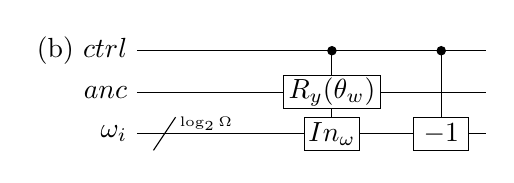
\begin{tikzpicture}[scale=1.000000,x=1pt,y=1pt]
\filldraw[color=white] (0.000000, -7.500000) rectangle (126.000000, 37.500000);
% Drawing wires
% Line 1: ctrl W \text{(b) }ctrl
\draw[color=black] (0.000000,30.000000) -- (126.000000,30.000000);
\draw[color=black] (0.000000,30.000000) node[left] {$\text{(b) }ctrl$};
% Line 2: anc W anc
\draw[color=black] (0.000000,15.000000) -- (126.000000,15.000000);
\draw[color=black] (0.000000,15.000000) node[left] {$anc$};
% Line 3: i W \omega_i
\draw[color=black] (0.000000,0.000000) -- (126.000000,0.000000);
\draw[color=black] (0.000000,0.000000) node[left] {$\omega_i$};
% Done with wires; drawing gates
% Line 5: i / ^{\log_2{\Omega}}
\draw (6.000000, -6.000000) -- (14.000000, 6.000000);
\draw (12.000000, 3.000000) node[right] {$\scriptstyle{^{\log_2{\Omega}}}$};
% Line 6: ctrl anc i LABEL
% Line 8: anc G:width=35 $R_y(\theta_w)$ i G:width=20 $In_\omega$ ctrl
\draw (70.500000,30.000000) -- (70.500000,0.000000);
\begin{scope}
\draw[fill=white] (70.500000, 15.000000) +(-45.000000:24.748737pt and 8.485281pt) -- +(45.000000:24.748737pt and 8.485281pt) -- +(135.000000:24.748737pt and 8.485281pt) -- +(225.000000:24.748737pt and 8.485281pt) -- cycle;
\clip (70.500000, 15.000000) +(-45.000000:24.748737pt and 8.485281pt) -- +(45.000000:24.748737pt and 8.485281pt) -- +(135.000000:24.748737pt and 8.485281pt) -- +(225.000000:24.748737pt and 8.485281pt) -- cycle;
\draw (70.500000, 15.000000) node {$R_y(\theta_w)$};
\end{scope}
\begin{scope}
\draw[fill=white] (70.500000, -0.000000) +(-45.000000:14.142136pt and 8.485281pt) -- +(45.000000:14.142136pt and 8.485281pt) -- +(135.000000:14.142136pt and 8.485281pt) -- +(225.000000:14.142136pt and 8.485281pt) -- cycle;
\clip (70.500000, -0.000000) +(-45.000000:14.142136pt and 8.485281pt) -- +(45.000000:14.142136pt and 8.485281pt) -- +(135.000000:14.142136pt and 8.485281pt) -- +(225.000000:14.142136pt and 8.485281pt) -- cycle;
\draw (70.500000, -0.000000) node {$In_\omega$};
\end{scope}
\filldraw (70.500000, 30.000000) circle(1.500000pt);
% Line 9: i G width=20 $-1$ ctrl
\draw (110.000000,30.000000) -- (110.000000,0.000000);
\begin{scope}
\draw[fill=white] (110.000000, -0.000000) +(-45.000000:14.142136pt and 8.485281pt) -- +(45.000000:14.142136pt and 8.485281pt) -- +(135.000000:14.142136pt and 8.485281pt) -- +(225.000000:14.142136pt and 8.485281pt) -- cycle;
\clip (110.000000, -0.000000) +(-45.000000:14.142136pt and 8.485281pt) -- +(45.000000:14.142136pt and 8.485281pt) -- +(135.000000:14.142136pt and 8.485281pt) -- +(225.000000:14.142136pt and 8.485281pt) -- cycle;
\draw (110.000000, -0.000000) node {$-1$};
\end{scope}
\filldraw (110.000000, 30.000000) circle(1.500000pt);
% Done with gates; drawing ending labels
% Done with ending labels; drawing cut lines and comments
% Done with comments
\end{tikzpicture}

    }
    \caption{
        \textbf{Bosonic Ladder Operator Block-Encoding}
        In subfigure (a), a block-encoding for the bosonic creation operator ($a_i^\dagger$) is given.
        In subfigure (b), a block-encoding for the bosonic annihilation operator ($a_i$) is given.
    }
    \label{fig:bosonic-ladder-op-be}
\end{figure}

The desired action of the block-encoding circuit for the bosonic creation operator is to increase the occupation of the bosonic mode by $1$ and rotate the block-encoding ancilla such that it has a coefficient of $\sqrt{\omega_i + 1 / \Omega}$ in the $\ket{0}$ state when the initial occupation of the $i^\text{th}$ bosonic mode is $w_i$.
This can be achieved by applying an incrementer to the the bosonic mode which increases the occupation by $1 \mod \Omega$ in each branch of the wavefunction.
The desired amplitudes of the block-encoding ancilla can be obtained using a series of $R_y$ gates that are controlled on the corresponding bosonic occupation.
An example circuit diagram is given in subfigure \ref{fig:bosonic-ladder-op-be}a.
A block-encoding for the bosonic annihilation operator can be constructed similarly, but with the block-encoding ancilla rotated prior to the occupation of the mode being decremented (subfigure \ref{fig:bosonic-ladder-op-be}b).

The angles of the $R_y$ gates are determined classically by the following function:
\begin{equation}
    \label{eq:single-op-angles}
    \theta(\omega_i) = 
    \begin{cases} 
        2 \cos^{-1}\Big(\sqrt{\omega_i/\Omega}\Big) & \text{when } \omega_i < \Omega\\
        \pi & \text{when } \omega_i = \Omega
    \end{cases}
\end{equation}
where $\omega_i$ here in comparison with $\omega_i + 1$ in Eq. \ref{eq:be-bos-creation} is due to the occupation of the state being updated prior to the rotations.


An implementation of a controlled incrementer circuit is given in \cite{Gidney_2015} which requires $\lceil \log_2\Omega \rceil - 1$ clean ancillae and $3 \lceil \log_2\Omega \rceil$ T gates.
The series of uniformly controlled rotations can be decomposed via the protocol given in Möttönen et. al \cite{mottonen2004transformation}.
A discussion of different schemes to construct a \textit{controlled} set of uniformly controlled rotations is given in Appendix \ref{sec:multiplexed-rotations}.
The resource estimates quoted in the remainder of this work assume the decomposition that requires $\Omega + 3$ uncontrolled rotations and $4 \lceil{\log_2{\Omega}}\rceil$ T gates (Figure \ref{fig:gate-optimized-controlled-multiplexed-rotations}).
In total, this block-encoding has a rescaling factor of $\sqrt{\Omega}$, requires one block-encoding ancilla and $\lceil{\log_2{\Omega}}\rceil$ clean ancillae, and uses $7 \lceil \log_2\Omega \rceil$ T gates and (at most) $\Omega + 3$ arbitrary rotations.


\subsection{Products of Bosonic Ladder Operators}

In this subsection, we discuss constructing block-encodings for a product of bosonic ladder operators acting on the same mode.
Unlike fermions, multiple bosons can occupy the same bosonic mode and a series of bosonic ladder operators can be applied to the state without necessarily zeroing-out the state.
Products of bosonic ladder operators acting on different modes can be block-encoded using Theorem \ref{th:product}.

Consider the desired action of a block-encoding for series of $R$ bosonic creation operators acting on the $i^\text{th}$ bosonic mode:
\begin{equation}
    \label{eq:be-S-creation-ops}
    U_{(a^\dagger_i)^R} \ket{\omega_i} \ket{0}_\text{anc} = 
    \begin{cases}
        \prod_{r=1}^{R} \sqrt{(\omega_i + r) / \Omega} \ket{\omega_i + R} \ket{0}_\text{anc} + \beta_\psi \ket{\perp} & \text{when } \omega_i \leq \Omega - R \\
        \ket{\perp} & \text{when } \omega_i > \Omega - R \\
    \end{cases}
\end{equation}

\begin{figure}
    \mbox{
        \include{figures/qpic-code/bosonic/products/R-creation}
        \include{figures/qpic-code/bosonic/products/S-annihilation}
    }
    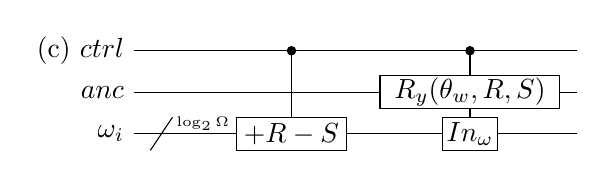
\begin{tikzpicture}[scale=1.000000,x=1pt,y=1pt]
\filldraw[color=white] (0.000000, -7.500000) rectangle (160.000000, 37.500000);
% Drawing wires
% Line 1: ctrl W \text{(c) }ctrl
\draw[color=black] (0.000000,30.000000) -- (160.000000,30.000000);
\draw[color=black] (0.000000,30.000000) node[left] {$\text{(c) }ctrl$};
% Line 2: anc W anc
\draw[color=black] (0.000000,15.000000) -- (160.000000,15.000000);
\draw[color=black] (0.000000,15.000000) node[left] {$anc$};
% Line 3: i W \omega_i
\draw[color=black] (0.000000,0.000000) -- (160.000000,0.000000);
\draw[color=black] (0.000000,0.000000) node[left] {$\omega_i$};
% Done with wires; drawing gates
% Line 5: i / ^{\log_2{\Omega}}
\draw (6.000000, -6.000000) -- (14.000000, 6.000000);
\draw (12.000000, 3.000000) node[right] {$\scriptstyle{^{\log_2{\Omega}}}$};
% Line 6: ctrl anc i LABEL width=-1
% Line 8: i G width=40 $+R-S$ ctrl
\draw (57.000000,30.000000) -- (57.000000,0.000000);
\begin{scope}
\draw[fill=white] (57.000000, -0.000000) +(-45.000000:28.284271pt and 8.485281pt) -- +(45.000000:28.284271pt and 8.485281pt) -- +(135.000000:28.284271pt and 8.485281pt) -- +(225.000000:28.284271pt and 8.485281pt) -- cycle;
\clip (57.000000, -0.000000) +(-45.000000:28.284271pt and 8.485281pt) -- +(45.000000:28.284271pt and 8.485281pt) -- +(135.000000:28.284271pt and 8.485281pt) -- +(225.000000:28.284271pt and 8.485281pt) -- cycle;
\draw (57.000000, -0.000000) node {$+R-S$};
\end{scope}
\filldraw (57.000000, 30.000000) circle(1.500000pt);
% Line 9: anc G:width=65 $R_y(\theta_w, R, S)$ i G:width=20 $In_\omega$ ctrl
\draw (121.500000,30.000000) -- (121.500000,0.000000);
\begin{scope}
\draw[fill=white] (121.500000, 15.000000) +(-45.000000:45.961941pt and 8.485281pt) -- +(45.000000:45.961941pt and 8.485281pt) -- +(135.000000:45.961941pt and 8.485281pt) -- +(225.000000:45.961941pt and 8.485281pt) -- cycle;
\clip (121.500000, 15.000000) +(-45.000000:45.961941pt and 8.485281pt) -- +(45.000000:45.961941pt and 8.485281pt) -- +(135.000000:45.961941pt and 8.485281pt) -- +(225.000000:45.961941pt and 8.485281pt) -- cycle;
\draw (121.500000, 15.000000) node {$R_y(\theta_w, R, S)$};
\end{scope}
\begin{scope}
\draw[fill=white] (121.500000, -0.000000) +(-45.000000:14.142136pt and 8.485281pt) -- +(45.000000:14.142136pt and 8.485281pt) -- +(135.000000:14.142136pt and 8.485281pt) -- +(225.000000:14.142136pt and 8.485281pt) -- cycle;
\clip (121.500000, -0.000000) +(-45.000000:14.142136pt and 8.485281pt) -- +(45.000000:14.142136pt and 8.485281pt) -- +(135.000000:14.142136pt and 8.485281pt) -- +(225.000000:14.142136pt and 8.485281pt) -- cycle;
\draw (121.500000, -0.000000) node {$In_\omega$};
\end{scope}
\filldraw (121.500000, 30.000000) circle(1.500000pt);
% Done with gates; drawing ending labels
% Done with ending labels; drawing cut lines and comments
% Done with comments
\end{tikzpicture}

    \caption{
        \textbf{Block-Encoding Product of Bosonic Ladder Operators}
        In subfigure (a), a block-encoding for the operator $(a_i^\dagger)^R$ is given.
        In subfigure (b), a block-encoding for the operator $(a_i)^S$ is given.
        In subfigure (c), a block-encoding for the operator $(a_i^\dagger)^R (a_i)^S$ is given.
    }
    \label{fig:products-bosonic-operators}
\end{figure}

A block-encoding for this operator can be achieved by updating the occupation of the bosonic mode by $+R$ and then performing a single series of rotations.
A circuit diagram for this construction is shown in subfigure \ref{fig:products-bosonic-operators}a.

The angles of the $R_y$ rotations are determined classically by the following function:
\begin{equation}
    \theta(\omega_i, R) = 
    \begin{cases} 
        2\cos^{-1}\Big(\prod_{r=0}^{R-1}\sqrt{(\omega_i - r) / \Omega}\Big) & \text{when } \omega_i \leq \Omega - R \\
        \pi & \text{when } \omega_i > \Omega - R
    \end{cases}
\end{equation}
where $\omega_i - r$ here in comparison with $\omega_i + r$ in Eq. \ref{eq:be-S-creation-ops} is due to the occupation of the state being updated prior to these rotations.

A block-encoding for a bosonic annihilation operator being applied $S$ times can be achieved using a similar construction shown in subfigue \ref{fig:products-bosonic-operators}b.
The occupation of the mode is first decreased by $S$ and then the controlled multiplexed rotations are applied to pick up the corresponding coefficient on the block-encoding ancilla.
The function to determine the rotation angles is given by:
\begin{equation}
    \theta(\omega_i, S) = 
    \begin{cases} 
        2\cos^{-1}\Big(\prod_{s=1}^{S}\sqrt{(\omega_i + s) / \Omega}\Big) & \text{when } \omega_i \geq S \\
        \pi & \text{when } \omega_i < S
    \end{cases}
\end{equation}

Likewise, a block-encoding for an operator of the form $(a_i^\dagger)^R (a_i)^S$ can be constructed using a similar form (subfigue \ref{fig:products-bosonic-operators}c).
The occupation of the mode is updated by a value of $+ R - S$ and then the controlled multiplexed rotations are applied to pick up the corresponding coefficient on the block-encoding ancilla.
The function to determine the rotation angles is given by:
\begin{equation}
    \theta(\omega_i, R, S) = 
    \begin{cases} 
        2\cos^{-1}\Big(\prod_{r=0}^{R-1}\sqrt{(\omega_i - r) / \Omega} \prod_{s=1}^{S}\sqrt{(\omega_i - R + s) / \Omega}\Big) & \text{when } S \leq \omega_i \leq \Omega - R \\
        \pi & \text{Otherwise} 
    \end{cases}
\end{equation}

Incrementing a quantum register by a classical value can be implemented in multiple ways with different compilations having different space-time tradeoffs.
The resource estimates presented in this work assume the compilation given in Figure \ref{fig:addition-gate-efficient}, which requires (at most) $3 \lceil \log_2 \Omega \rceil$ T gates.
In total, these block-encoding circuits have a rescaling factor of $\lambda = \Omega^{(R+S)/2}$, require one block-encoding ancilla and $\lceil{\log_2{\Omega}}\rceil$ clean ancillae, and use (at most) $7 \lceil \log_2 \Omega \rceil$ T gates and $\Omega + 3$ arbitrary rotations.


\subsection{Linear Combinations of Bosonic Ladder Operators}

In this subsection, we discuss constructing block-encodings for a linear combination of a product of bosonic ladder operators with its hermitian conjugate.


\begin{figure}
    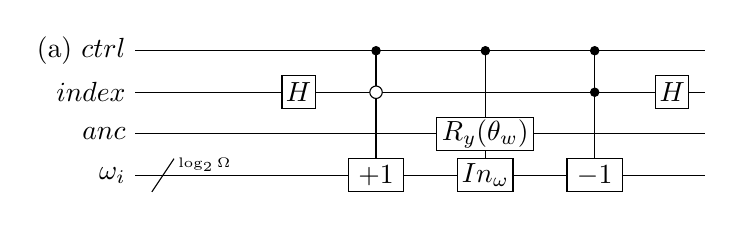
\begin{tikzpicture}[scale=1.000000,x=1pt,y=1pt]
\filldraw[color=white] (0.000000, -7.500000) rectangle (206.000000, 52.500000);
% Drawing wires
% Line 1: ctrl W \text{(a) }ctrl
\draw[color=black] (0.000000,45.000000) -- (206.000000,45.000000);
\draw[color=black] (0.000000,45.000000) node[left] {$\text{(a) }ctrl$};
% Line 2: index W index
\draw[color=black] (0.000000,30.000000) -- (206.000000,30.000000);
\draw[color=black] (0.000000,30.000000) node[left] {$index$};
% Line 3: anc W anc
\draw[color=black] (0.000000,15.000000) -- (206.000000,15.000000);
\draw[color=black] (0.000000,15.000000) node[left] {$anc$};
% Line 4: i W \omega_i
\draw[color=black] (0.000000,0.000000) -- (206.000000,0.000000);
\draw[color=black] (0.000000,0.000000) node[left] {$\omega_i$};
% Done with wires; drawing gates
% Line 6: i / ^{\log_2{\Omega}}
\draw (6.000000, -6.000000) -- (14.000000, 6.000000);
\draw (12.000000, 3.000000) node[right] {$\scriptstyle{^{\log_2{\Omega}}}$};
% Line 7: ctrl anc index i LABEL
% Line 9: index G $H$
\begin{scope}
\draw[fill=white] (59.000000, 30.000000) +(-45.000000:8.485281pt and 8.485281pt) -- +(45.000000:8.485281pt and 8.485281pt) -- +(135.000000:8.485281pt and 8.485281pt) -- +(225.000000:8.485281pt and 8.485281pt) -- cycle;
\clip (59.000000, 30.000000) +(-45.000000:8.485281pt and 8.485281pt) -- +(45.000000:8.485281pt and 8.485281pt) -- +(135.000000:8.485281pt and 8.485281pt) -- +(225.000000:8.485281pt and 8.485281pt) -- cycle;
\draw (59.000000, 30.000000) node {$H$};
\end{scope}
% Line 10: i G width=20 $+1$ ctrl -index
\draw (87.000000,45.000000) -- (87.000000,0.000000);
\begin{scope}
\draw[fill=white] (87.000000, -0.000000) +(-45.000000:14.142136pt and 8.485281pt) -- +(45.000000:14.142136pt and 8.485281pt) -- +(135.000000:14.142136pt and 8.485281pt) -- +(225.000000:14.142136pt and 8.485281pt) -- cycle;
\clip (87.000000, -0.000000) +(-45.000000:14.142136pt and 8.485281pt) -- +(45.000000:14.142136pt and 8.485281pt) -- +(135.000000:14.142136pt and 8.485281pt) -- +(225.000000:14.142136pt and 8.485281pt) -- cycle;
\draw (87.000000, -0.000000) node {$+1$};
\end{scope}
\filldraw (87.000000, 45.000000) circle(1.500000pt);
\draw[fill=white] (87.000000, 30.000000) circle(2.250000pt);
% Line 11: anc G:width=35 $R_y(\theta_w)$ i G:width=20 $In_\omega$ ctrl
\draw (126.500000,45.000000) -- (126.500000,0.000000);
\begin{scope}
\draw[fill=white] (126.500000, 15.000000) +(-45.000000:24.748737pt and 8.485281pt) -- +(45.000000:24.748737pt and 8.485281pt) -- +(135.000000:24.748737pt and 8.485281pt) -- +(225.000000:24.748737pt and 8.485281pt) -- cycle;
\clip (126.500000, 15.000000) +(-45.000000:24.748737pt and 8.485281pt) -- +(45.000000:24.748737pt and 8.485281pt) -- +(135.000000:24.748737pt and 8.485281pt) -- +(225.000000:24.748737pt and 8.485281pt) -- cycle;
\draw (126.500000, 15.000000) node {$R_y(\theta_w)$};
\end{scope}
\begin{scope}
\draw[fill=white] (126.500000, -0.000000) +(-45.000000:14.142136pt and 8.485281pt) -- +(45.000000:14.142136pt and 8.485281pt) -- +(135.000000:14.142136pt and 8.485281pt) -- +(225.000000:14.142136pt and 8.485281pt) -- cycle;
\clip (126.500000, -0.000000) +(-45.000000:14.142136pt and 8.485281pt) -- +(45.000000:14.142136pt and 8.485281pt) -- +(135.000000:14.142136pt and 8.485281pt) -- +(225.000000:14.142136pt and 8.485281pt) -- cycle;
\draw (126.500000, -0.000000) node {$In_\omega$};
\end{scope}
\filldraw (126.500000, 45.000000) circle(1.500000pt);
% Line 12: i G width=20 $-1$ ctrl index
\draw (166.000000,45.000000) -- (166.000000,0.000000);
\begin{scope}
\draw[fill=white] (166.000000, -0.000000) +(-45.000000:14.142136pt and 8.485281pt) -- +(45.000000:14.142136pt and 8.485281pt) -- +(135.000000:14.142136pt and 8.485281pt) -- +(225.000000:14.142136pt and 8.485281pt) -- cycle;
\clip (166.000000, -0.000000) +(-45.000000:14.142136pt and 8.485281pt) -- +(45.000000:14.142136pt and 8.485281pt) -- +(135.000000:14.142136pt and 8.485281pt) -- +(225.000000:14.142136pt and 8.485281pt) -- cycle;
\draw (166.000000, -0.000000) node {$-1$};
\end{scope}
\filldraw (166.000000, 45.000000) circle(1.500000pt);
\filldraw (166.000000, 30.000000) circle(1.500000pt);
% Line 13: index G $H$
\begin{scope}
\draw[fill=white] (194.000000, 30.000000) +(-45.000000:8.485281pt and 8.485281pt) -- +(45.000000:8.485281pt and 8.485281pt) -- +(135.000000:8.485281pt and 8.485281pt) -- +(225.000000:8.485281pt and 8.485281pt) -- cycle;
\clip (194.000000, 30.000000) +(-45.000000:8.485281pt and 8.485281pt) -- +(45.000000:8.485281pt and 8.485281pt) -- +(135.000000:8.485281pt and 8.485281pt) -- +(225.000000:8.485281pt and 8.485281pt) -- cycle;
\draw (194.000000, 30.000000) node {$H$};
\end{scope}
% Done with gates; drawing ending labels
% Done with ending labels; drawing cut lines and comments
% Done with comments
\end{tikzpicture}

    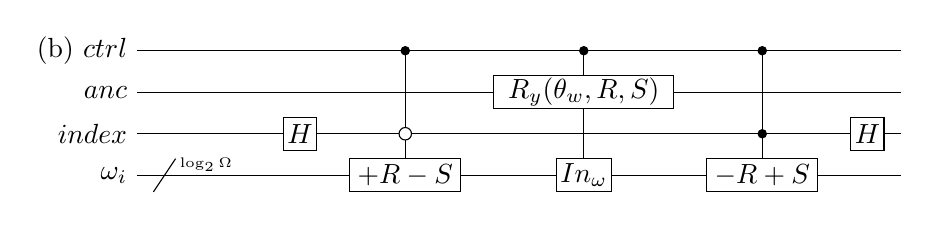
\begin{tikzpicture}[scale=1.000000,x=1pt,y=1pt]
\filldraw[color=white] (0.000000, -7.500000) rectangle (276.000000, 52.500000);
% Drawing wires
% Line 1: ctrl W \text{(b) }ctrl
\draw[color=black] (0.000000,45.000000) -- (276.000000,45.000000);
\draw[color=black] (0.000000,45.000000) node[left] {$\text{(b) }ctrl$};
% Line 2: anc W anc
\draw[color=black] (0.000000,30.000000) -- (276.000000,30.000000);
\draw[color=black] (0.000000,30.000000) node[left] {$anc$};
% Line 3: index W index
\draw[color=black] (0.000000,15.000000) -- (276.000000,15.000000);
\draw[color=black] (0.000000,15.000000) node[left] {$index$};
% Line 4: i W \omega_i
\draw[color=black] (0.000000,0.000000) -- (276.000000,0.000000);
\draw[color=black] (0.000000,0.000000) node[left] {$\omega_i$};
% Done with wires; drawing gates
% Line 6: i / ^{\log_2{\Omega}}
\draw (6.000000, -6.000000) -- (14.000000, 6.000000);
\draw (12.000000, 3.000000) node[right] {$\scriptstyle{^{\log_2{\Omega}}}$};
% Line 7: ctrl anc index i LABEL
% Line 9: index G $H$
\begin{scope}
\draw[fill=white] (59.000000, 15.000000) +(-45.000000:8.485281pt and 8.485281pt) -- +(45.000000:8.485281pt and 8.485281pt) -- +(135.000000:8.485281pt and 8.485281pt) -- +(225.000000:8.485281pt and 8.485281pt) -- cycle;
\clip (59.000000, 15.000000) +(-45.000000:8.485281pt and 8.485281pt) -- +(45.000000:8.485281pt and 8.485281pt) -- +(135.000000:8.485281pt and 8.485281pt) -- +(225.000000:8.485281pt and 8.485281pt) -- cycle;
\draw (59.000000, 15.000000) node {$H$};
\end{scope}
% Line 10: i G width=40 $+R-S$ ctrl -index
\draw (97.000000,45.000000) -- (97.000000,0.000000);
\begin{scope}
\draw[fill=white] (97.000000, -0.000000) +(-45.000000:28.284271pt and 8.485281pt) -- +(45.000000:28.284271pt and 8.485281pt) -- +(135.000000:28.284271pt and 8.485281pt) -- +(225.000000:28.284271pt and 8.485281pt) -- cycle;
\clip (97.000000, -0.000000) +(-45.000000:28.284271pt and 8.485281pt) -- +(45.000000:28.284271pt and 8.485281pt) -- +(135.000000:28.284271pt and 8.485281pt) -- +(225.000000:28.284271pt and 8.485281pt) -- cycle;
\draw (97.000000, -0.000000) node {$+R-S$};
\end{scope}
\filldraw (97.000000, 45.000000) circle(1.500000pt);
\draw[fill=white] (97.000000, 15.000000) circle(2.250000pt);
% Line 11: anc G:width=65 $R_y(\theta_w, R, S)$ i G:width=20 $In_\omega$ ctrl
\draw (161.500000,45.000000) -- (161.500000,0.000000);
\begin{scope}
\draw[fill=white] (161.500000, 30.000000) +(-45.000000:45.961941pt and 8.485281pt) -- +(45.000000:45.961941pt and 8.485281pt) -- +(135.000000:45.961941pt and 8.485281pt) -- +(225.000000:45.961941pt and 8.485281pt) -- cycle;
\clip (161.500000, 30.000000) +(-45.000000:45.961941pt and 8.485281pt) -- +(45.000000:45.961941pt and 8.485281pt) -- +(135.000000:45.961941pt and 8.485281pt) -- +(225.000000:45.961941pt and 8.485281pt) -- cycle;
\draw (161.500000, 30.000000) node {$R_y(\theta_w, R, S)$};
\end{scope}
\begin{scope}
\draw[fill=white] (161.500000, -0.000000) +(-45.000000:14.142136pt and 8.485281pt) -- +(45.000000:14.142136pt and 8.485281pt) -- +(135.000000:14.142136pt and 8.485281pt) -- +(225.000000:14.142136pt and 8.485281pt) -- cycle;
\clip (161.500000, -0.000000) +(-45.000000:14.142136pt and 8.485281pt) -- +(45.000000:14.142136pt and 8.485281pt) -- +(135.000000:14.142136pt and 8.485281pt) -- +(225.000000:14.142136pt and 8.485281pt) -- cycle;
\draw (161.500000, -0.000000) node {$In_\omega$};
\end{scope}
\filldraw (161.500000, 45.000000) circle(1.500000pt);
% Line 12: i G width=40 $-R+S$ ctrl index
\draw (226.000000,45.000000) -- (226.000000,0.000000);
\begin{scope}
\draw[fill=white] (226.000000, -0.000000) +(-45.000000:28.284271pt and 8.485281pt) -- +(45.000000:28.284271pt and 8.485281pt) -- +(135.000000:28.284271pt and 8.485281pt) -- +(225.000000:28.284271pt and 8.485281pt) -- cycle;
\clip (226.000000, -0.000000) +(-45.000000:28.284271pt and 8.485281pt) -- +(45.000000:28.284271pt and 8.485281pt) -- +(135.000000:28.284271pt and 8.485281pt) -- +(225.000000:28.284271pt and 8.485281pt) -- cycle;
\draw (226.000000, -0.000000) node {$-R+S$};
\end{scope}
\filldraw (226.000000, 45.000000) circle(1.500000pt);
\filldraw (226.000000, 15.000000) circle(1.500000pt);
% Line 13: index G $H$
\begin{scope}
\draw[fill=white] (264.000000, 15.000000) +(-45.000000:8.485281pt and 8.485281pt) -- +(45.000000:8.485281pt and 8.485281pt) -- +(135.000000:8.485281pt and 8.485281pt) -- +(225.000000:8.485281pt and 8.485281pt) -- cycle;
\clip (264.000000, 15.000000) +(-45.000000:8.485281pt and 8.485281pt) -- +(45.000000:8.485281pt and 8.485281pt) -- +(135.000000:8.485281pt and 8.485281pt) -- +(225.000000:8.485281pt and 8.485281pt) -- cycle;
\draw (264.000000, 15.000000) node {$H$};
\end{scope}
% Done with gates; drawing ending labels
% Done with ending labels; drawing cut lines and comments
% Done with comments
\end{tikzpicture}

    \caption{
        \textbf{Block-Encoding Product of Bosonic Ladder Operators Plus Hermitian Conjugate}
        In subfigure (a), a block-encoding for the operator $(a_i^\dagger + a_i)$ is given.
        In subfigure (b), a block-encoding for the operator $\big((a_i^\dagger)^R (a_i)^S + (a_i^\dagger)^S (a_i)^R\big)$ is given.
    }
    \label{fig:lc-bosonic}
\end{figure}


Consider the block-encodings for the operators $a_i^\dagger$ and $a_i$.
An efficient block-encoding of the operator $a_i^\dagger + a_i$ can be constructed using the symmetry between the two individual block-encodings. 
To apply the creation operator, the occupancy is increased by $1$ and then the rotations are applied, whereas for the annihilation operator, the rotations are applied first and then the occupancy is decreased by $1$.
Since the desired rotation angles are independent of which operator is being applied (Eq. \ref{eq:single-op-angles}), we can apply these rotations once for both operators.
However, one additional block-encoding ancilla is required to index between the two operators.
An example circuit diagram for this construction is shown in subfigue \ref{fig:lc-bosonic}a.
A block-encoding for the generalized operator $\big((a_i^\dagger)^R (a_i)^S + (a_i^\dagger)^S (a_i)^R\big)$ can be constructed similarly and is shown in subfigure \ref{fig:lc-bosonic}b.

\begin{figure}
    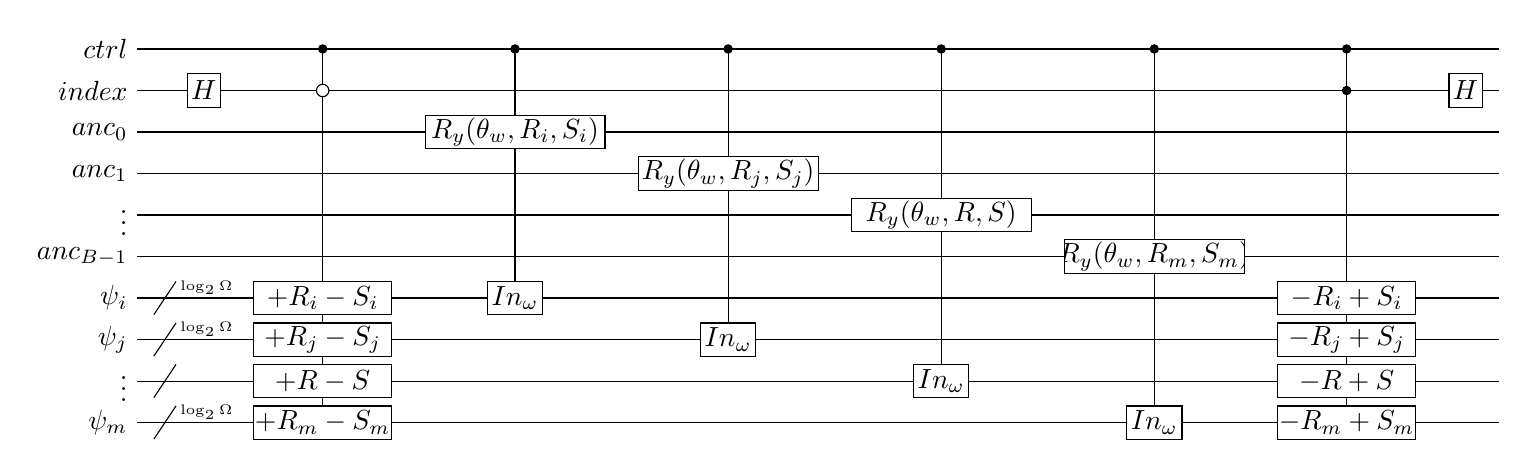
\begin{tikzpicture}[scale=1.000000,x=1pt,y=1pt]
\filldraw[color=white] (0.000000, -7.500000) rectangle (492.000000, 142.500000);
% Drawing wires
% Line 1: ctrl W ctrl
\draw[color=black] (0.000000,135.000000) -- (492.000000,135.000000);
\draw[color=black] (0.000000,135.000000) node[left] {$ctrl$};
% Line 2: index W index
\draw[color=black] (0.000000,120.000000) -- (492.000000,120.000000);
\draw[color=black] (0.000000,120.000000) node[left] {$index$};
% Line 3: anc_0 W anc_0
\draw[color=black] (0.000000,105.000000) -- (492.000000,105.000000);
\draw[color=black] (0.000000,105.000000) node[left] {$anc_0$};
% Line 4: anc_1 W anc_1
\draw[color=black] (0.000000,90.000000) -- (492.000000,90.000000);
\draw[color=black] (0.000000,90.000000) node[left] {$anc_1$};
% Line 5: anc_series W \vdots
\draw[color=black] (0.000000,75.000000) -- (492.000000,75.000000);
\draw[color=black] (0.000000,75.000000) node[left] {$\vdots$};
% Line 6: anc_B W anc_{B-1}
\draw[color=black] (0.000000,60.000000) -- (492.000000,60.000000);
\draw[color=black] (0.000000,60.000000) node[left] {$anc_{B-1}$};
% Line 8: i W \psi_i
\draw[color=black] (0.000000,45.000000) -- (492.000000,45.000000);
\draw[color=black] (0.000000,45.000000) node[left] {$\psi_i$};
% Line 9: j W \psi_j
\draw[color=black] (0.000000,30.000000) -- (492.000000,30.000000);
\draw[color=black] (0.000000,30.000000) node[left] {$\psi_j$};
% Line 10: sys_series W \vdots
\draw[color=black] (0.000000,15.000000) -- (492.000000,15.000000);
\draw[color=black] (0.000000,15.000000) node[left] {$\vdots$};
% Line 11: m W \psi_m
\draw[color=black] (0.000000,0.000000) -- (492.000000,0.000000);
\draw[color=black] (0.000000,0.000000) node[left] {$\psi_m$};
% Done with wires; drawing gates
% Line 13: i / ^{\log_2{\Omega}}
\draw (6.000000, 39.000000) -- (14.000000, 51.000000);
\draw (12.000000, 48.000000) node[right] {$\scriptstyle{^{\log_2{\Omega}}}$};
% Line 14: j / ^{\log_2{\Omega}}
\draw (6.000000, 24.000000) -- (14.000000, 36.000000);
\draw (12.000000, 33.000000) node[right] {$\scriptstyle{^{\log_2{\Omega}}}$};
% Line 15: sys_series /
\draw (6.000000, 9.000000) -- (14.000000, 21.000000);
% Line 16: m / ^{\log_2{\Omega}}
\draw (6.000000, -6.000000) -- (14.000000, 6.000000);
\draw (12.000000, 3.000000) node[right] {$\scriptstyle{^{\log_2{\Omega}}}$};
% Line 18: ctrl index anc_0 anc_1 anc_series anc_B i j sys_series m LABEL width=-20
% Line 20: index G $H$
\begin{scope}
\draw[fill=white] (24.000000, 120.000000) +(-45.000000:8.485281pt and 8.485281pt) -- +(45.000000:8.485281pt and 8.485281pt) -- +(135.000000:8.485281pt and 8.485281pt) -- +(225.000000:8.485281pt and 8.485281pt) -- cycle;
\clip (24.000000, 120.000000) +(-45.000000:8.485281pt and 8.485281pt) -- +(45.000000:8.485281pt and 8.485281pt) -- +(135.000000:8.485281pt and 8.485281pt) -- +(225.000000:8.485281pt and 8.485281pt) -- cycle;
\draw (24.000000, 120.000000) node {$H$};
\end{scope}
% Line 22: i G width=50 $+R_i-S_i$ j G width=50 $+R_j-S_j$ sys_series G width=50 $+R-S$ m G width=50 $+R_m-S_m$ ctrl -index
\draw (67.000000,135.000000) -- (67.000000,0.000000);
\begin{scope}
\draw[fill=white] (67.000000, 45.000000) +(-45.000000:35.355339pt and 8.485281pt) -- +(45.000000:35.355339pt and 8.485281pt) -- +(135.000000:35.355339pt and 8.485281pt) -- +(225.000000:35.355339pt and 8.485281pt) -- cycle;
\clip (67.000000, 45.000000) +(-45.000000:35.355339pt and 8.485281pt) -- +(45.000000:35.355339pt and 8.485281pt) -- +(135.000000:35.355339pt and 8.485281pt) -- +(225.000000:35.355339pt and 8.485281pt) -- cycle;
\draw (67.000000, 45.000000) node {$+R_i-S_i$};
\end{scope}
\begin{scope}
\draw[fill=white] (67.000000, 30.000000) +(-45.000000:35.355339pt and 8.485281pt) -- +(45.000000:35.355339pt and 8.485281pt) -- +(135.000000:35.355339pt and 8.485281pt) -- +(225.000000:35.355339pt and 8.485281pt) -- cycle;
\clip (67.000000, 30.000000) +(-45.000000:35.355339pt and 8.485281pt) -- +(45.000000:35.355339pt and 8.485281pt) -- +(135.000000:35.355339pt and 8.485281pt) -- +(225.000000:35.355339pt and 8.485281pt) -- cycle;
\draw (67.000000, 30.000000) node {$+R_j-S_j$};
\end{scope}
\begin{scope}
\draw[fill=white] (67.000000, 15.000000) +(-45.000000:35.355339pt and 8.485281pt) -- +(45.000000:35.355339pt and 8.485281pt) -- +(135.000000:35.355339pt and 8.485281pt) -- +(225.000000:35.355339pt and 8.485281pt) -- cycle;
\clip (67.000000, 15.000000) +(-45.000000:35.355339pt and 8.485281pt) -- +(45.000000:35.355339pt and 8.485281pt) -- +(135.000000:35.355339pt and 8.485281pt) -- +(225.000000:35.355339pt and 8.485281pt) -- cycle;
\draw (67.000000, 15.000000) node {$+R-S$};
\end{scope}
\begin{scope}
\draw[fill=white] (67.000000, -0.000000) +(-45.000000:35.355339pt and 8.485281pt) -- +(45.000000:35.355339pt and 8.485281pt) -- +(135.000000:35.355339pt and 8.485281pt) -- +(225.000000:35.355339pt and 8.485281pt) -- cycle;
\clip (67.000000, -0.000000) +(-45.000000:35.355339pt and 8.485281pt) -- +(45.000000:35.355339pt and 8.485281pt) -- +(135.000000:35.355339pt and 8.485281pt) -- +(225.000000:35.355339pt and 8.485281pt) -- cycle;
\draw (67.000000, -0.000000) node {$+R_m-S_m$};
\end{scope}
\filldraw (67.000000, 135.000000) circle(1.500000pt);
\draw[fill=white] (67.000000, 120.000000) circle(2.250000pt);
% Line 24: anc_0 G:width=65 $R_y(\theta_w, R_i, S_i)$ i G:width=20 $In_\omega$ ctrl
\draw (136.500000,135.000000) -- (136.500000,45.000000);
\begin{scope}
\draw[fill=white] (136.500000, 105.000000) +(-45.000000:45.961941pt and 8.485281pt) -- +(45.000000:45.961941pt and 8.485281pt) -- +(135.000000:45.961941pt and 8.485281pt) -- +(225.000000:45.961941pt and 8.485281pt) -- cycle;
\clip (136.500000, 105.000000) +(-45.000000:45.961941pt and 8.485281pt) -- +(45.000000:45.961941pt and 8.485281pt) -- +(135.000000:45.961941pt and 8.485281pt) -- +(225.000000:45.961941pt and 8.485281pt) -- cycle;
\draw (136.500000, 105.000000) node {$R_y(\theta_w, R_i, S_i)$};
\end{scope}
\begin{scope}
\draw[fill=white] (136.500000, 45.000000) +(-45.000000:14.142136pt and 8.485281pt) -- +(45.000000:14.142136pt and 8.485281pt) -- +(135.000000:14.142136pt and 8.485281pt) -- +(225.000000:14.142136pt and 8.485281pt) -- cycle;
\clip (136.500000, 45.000000) +(-45.000000:14.142136pt and 8.485281pt) -- +(45.000000:14.142136pt and 8.485281pt) -- +(135.000000:14.142136pt and 8.485281pt) -- +(225.000000:14.142136pt and 8.485281pt) -- cycle;
\draw (136.500000, 45.000000) node {$In_\omega$};
\end{scope}
\filldraw (136.500000, 135.000000) circle(1.500000pt);
% Line 25: anc_1 G:width=65 $R_y(\theta_w, R_j, S_j)$ j G:width=20 $In_\omega$ ctrl
\draw (213.500000,135.000000) -- (213.500000,30.000000);
\begin{scope}
\draw[fill=white] (213.500000, 90.000000) +(-45.000000:45.961941pt and 8.485281pt) -- +(45.000000:45.961941pt and 8.485281pt) -- +(135.000000:45.961941pt and 8.485281pt) -- +(225.000000:45.961941pt and 8.485281pt) -- cycle;
\clip (213.500000, 90.000000) +(-45.000000:45.961941pt and 8.485281pt) -- +(45.000000:45.961941pt and 8.485281pt) -- +(135.000000:45.961941pt and 8.485281pt) -- +(225.000000:45.961941pt and 8.485281pt) -- cycle;
\draw (213.500000, 90.000000) node {$R_y(\theta_w, R_j, S_j)$};
\end{scope}
\begin{scope}
\draw[fill=white] (213.500000, 30.000000) +(-45.000000:14.142136pt and 8.485281pt) -- +(45.000000:14.142136pt and 8.485281pt) -- +(135.000000:14.142136pt and 8.485281pt) -- +(225.000000:14.142136pt and 8.485281pt) -- cycle;
\clip (213.500000, 30.000000) +(-45.000000:14.142136pt and 8.485281pt) -- +(45.000000:14.142136pt and 8.485281pt) -- +(135.000000:14.142136pt and 8.485281pt) -- +(225.000000:14.142136pt and 8.485281pt) -- cycle;
\draw (213.500000, 30.000000) node {$In_\omega$};
\end{scope}
\filldraw (213.500000, 135.000000) circle(1.500000pt);
% Line 26: anc_series G:width=65 $R_y(\theta_w, R, S)$ sys_series G:width=20 $In_\omega$ ctrl
\draw (290.500000,135.000000) -- (290.500000,15.000000);
\begin{scope}
\draw[fill=white] (290.500000, 75.000000) +(-45.000000:45.961941pt and 8.485281pt) -- +(45.000000:45.961941pt and 8.485281pt) -- +(135.000000:45.961941pt and 8.485281pt) -- +(225.000000:45.961941pt and 8.485281pt) -- cycle;
\clip (290.500000, 75.000000) +(-45.000000:45.961941pt and 8.485281pt) -- +(45.000000:45.961941pt and 8.485281pt) -- +(135.000000:45.961941pt and 8.485281pt) -- +(225.000000:45.961941pt and 8.485281pt) -- cycle;
\draw (290.500000, 75.000000) node {$R_y(\theta_w, R, S)$};
\end{scope}
\begin{scope}
\draw[fill=white] (290.500000, 15.000000) +(-45.000000:14.142136pt and 8.485281pt) -- +(45.000000:14.142136pt and 8.485281pt) -- +(135.000000:14.142136pt and 8.485281pt) -- +(225.000000:14.142136pt and 8.485281pt) -- cycle;
\clip (290.500000, 15.000000) +(-45.000000:14.142136pt and 8.485281pt) -- +(45.000000:14.142136pt and 8.485281pt) -- +(135.000000:14.142136pt and 8.485281pt) -- +(225.000000:14.142136pt and 8.485281pt) -- cycle;
\draw (290.500000, 15.000000) node {$In_\omega$};
\end{scope}
\filldraw (290.500000, 135.000000) circle(1.500000pt);
% Line 27: anc_B G:width=65 $R_y(\theta_w, R_m, S_m)$ m G:width=20 $In_\omega$ ctrl
\draw (367.500000,135.000000) -- (367.500000,0.000000);
\begin{scope}
\draw[fill=white] (367.500000, 60.000000) +(-45.000000:45.961941pt and 8.485281pt) -- +(45.000000:45.961941pt and 8.485281pt) -- +(135.000000:45.961941pt and 8.485281pt) -- +(225.000000:45.961941pt and 8.485281pt) -- cycle;
\clip (367.500000, 60.000000) +(-45.000000:45.961941pt and 8.485281pt) -- +(45.000000:45.961941pt and 8.485281pt) -- +(135.000000:45.961941pt and 8.485281pt) -- +(225.000000:45.961941pt and 8.485281pt) -- cycle;
\draw (367.500000, 60.000000) node {$R_y(\theta_w, R_m, S_m)$};
\end{scope}
\begin{scope}
\draw[fill=white] (367.500000, -0.000000) +(-45.000000:14.142136pt and 8.485281pt) -- +(45.000000:14.142136pt and 8.485281pt) -- +(135.000000:14.142136pt and 8.485281pt) -- +(225.000000:14.142136pt and 8.485281pt) -- cycle;
\clip (367.500000, -0.000000) +(-45.000000:14.142136pt and 8.485281pt) -- +(45.000000:14.142136pt and 8.485281pt) -- +(135.000000:14.142136pt and 8.485281pt) -- +(225.000000:14.142136pt and 8.485281pt) -- cycle;
\draw (367.500000, -0.000000) node {$In_\omega$};
\end{scope}
\filldraw (367.500000, 135.000000) circle(1.500000pt);
% Line 29: i G width=50 $-R_i+S_i$ j G width=50 $-R_j+S_j$ sys_series G width=50 $-R+S$ m G width=50 $-R_m+S_m$ ctrl index
\draw (437.000000,135.000000) -- (437.000000,0.000000);
\begin{scope}
\draw[fill=white] (437.000000, 45.000000) +(-45.000000:35.355339pt and 8.485281pt) -- +(45.000000:35.355339pt and 8.485281pt) -- +(135.000000:35.355339pt and 8.485281pt) -- +(225.000000:35.355339pt and 8.485281pt) -- cycle;
\clip (437.000000, 45.000000) +(-45.000000:35.355339pt and 8.485281pt) -- +(45.000000:35.355339pt and 8.485281pt) -- +(135.000000:35.355339pt and 8.485281pt) -- +(225.000000:35.355339pt and 8.485281pt) -- cycle;
\draw (437.000000, 45.000000) node {$-R_i+S_i$};
\end{scope}
\begin{scope}
\draw[fill=white] (437.000000, 30.000000) +(-45.000000:35.355339pt and 8.485281pt) -- +(45.000000:35.355339pt and 8.485281pt) -- +(135.000000:35.355339pt and 8.485281pt) -- +(225.000000:35.355339pt and 8.485281pt) -- cycle;
\clip (437.000000, 30.000000) +(-45.000000:35.355339pt and 8.485281pt) -- +(45.000000:35.355339pt and 8.485281pt) -- +(135.000000:35.355339pt and 8.485281pt) -- +(225.000000:35.355339pt and 8.485281pt) -- cycle;
\draw (437.000000, 30.000000) node {$-R_j+S_j$};
\end{scope}
\begin{scope}
\draw[fill=white] (437.000000, 15.000000) +(-45.000000:35.355339pt and 8.485281pt) -- +(45.000000:35.355339pt and 8.485281pt) -- +(135.000000:35.355339pt and 8.485281pt) -- +(225.000000:35.355339pt and 8.485281pt) -- cycle;
\clip (437.000000, 15.000000) +(-45.000000:35.355339pt and 8.485281pt) -- +(45.000000:35.355339pt and 8.485281pt) -- +(135.000000:35.355339pt and 8.485281pt) -- +(225.000000:35.355339pt and 8.485281pt) -- cycle;
\draw (437.000000, 15.000000) node {$-R+S$};
\end{scope}
\begin{scope}
\draw[fill=white] (437.000000, -0.000000) +(-45.000000:35.355339pt and 8.485281pt) -- +(45.000000:35.355339pt and 8.485281pt) -- +(135.000000:35.355339pt and 8.485281pt) -- +(225.000000:35.355339pt and 8.485281pt) -- cycle;
\clip (437.000000, -0.000000) +(-45.000000:35.355339pt and 8.485281pt) -- +(45.000000:35.355339pt and 8.485281pt) -- +(135.000000:35.355339pt and 8.485281pt) -- +(225.000000:35.355339pt and 8.485281pt) -- cycle;
\draw (437.000000, -0.000000) node {$-R_m+S_m$};
\end{scope}
\filldraw (437.000000, 135.000000) circle(1.500000pt);
\filldraw (437.000000, 120.000000) circle(1.500000pt);
% Line 31: index G $H$
\begin{scope}
\draw[fill=white] (480.000000, 120.000000) +(-45.000000:8.485281pt and 8.485281pt) -- +(45.000000:8.485281pt and 8.485281pt) -- +(135.000000:8.485281pt and 8.485281pt) -- +(225.000000:8.485281pt and 8.485281pt) -- cycle;
\clip (480.000000, 120.000000) +(-45.000000:8.485281pt and 8.485281pt) -- +(45.000000:8.485281pt and 8.485281pt) -- +(135.000000:8.485281pt and 8.485281pt) -- +(225.000000:8.485281pt and 8.485281pt) -- cycle;
\draw (480.000000, 120.000000) node {$H$};
\end{scope}
% Done with gates; drawing ending labels
% Done with ending labels; drawing cut lines and comments
% Done with comments
\end{tikzpicture}

    \caption{
        \textbf{Generalized Block-Encoding Product of Bosonic Ladder Operators Plus Hermitian Conjugate}
        A block-encoding for the operator $((a_i^\dagger)^{R_i} + a_i^{S_i})((a_j^\dagger)^{R_j} + a_j^{S_j})...((a_m^\dagger)^{R_m} + a_m^{S_m}) + h.c.$ is given.
    }
    \label{fig:lc-bosonic-general}
\end{figure}

Likewise, this construction can be generalized to a linear combination of a product of bosonic operators acting on different modes plus its hermitian conjugate.
An example circuit diagram for this construction is shown in Figure \ref{fig:lc-bosonic-general}.
For an operator acting on $B$ bosonic modes, these block-encodings have a rescaling factor of $\lambda = 2 \Omega^{T/2}$ where $T$ is the sum of the exponents of the operators in a term: $T = \sum_{b=0}^{B-1}(R_b+S_b)$.
Additionally, they require $B+1$ block-encoding ancillae and $\lceil{\log_2{\Omega}}\rceil + 1$ clean ancillae, and use (at most) $12B \lceil \log_2 \Omega \rceil + - 4(B - 1)$ T gates and $B(\Omega + 3)$ arbitrary rotations.


\subsection{Terms with Fermionic and Bosonic Ladder Operators}

In the previous subsections, we discussed strategies for compiling block-encodings of different operators acting on either fermionic or bosonic modes.
In this subsection, we discuss block-encodings for operators that contain operators that act on both fermionic and bosonic operators.

\begin{figure}
    % 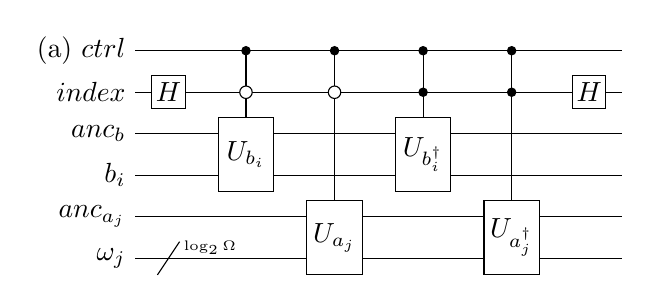
\begin{tikzpicture}[scale=1.000000,x=1pt,y=1pt]
\filldraw[color=white] (0.000000, -7.500000) rectangle (176.000000, 82.500000);
% Drawing wires
% Line 1: ctrl W \text{(a) }ctrl
\draw[color=black] (0.000000,75.000000) -- (176.000000,75.000000);
\draw[color=black] (0.000000,75.000000) node[left] {$\text{(a) }ctrl$};
% Line 2: index W index
\draw[color=black] (0.000000,60.000000) -- (176.000000,60.000000);
\draw[color=black] (0.000000,60.000000) node[left] {$index$};
% Line 3: anc_b W anc_b
\draw[color=black] (0.000000,45.000000) -- (176.000000,45.000000);
\draw[color=black] (0.000000,45.000000) node[left] {$anc_b$};
% Line 4: i W b_i
\draw[color=black] (0.000000,30.000000) -- (176.000000,30.000000);
\draw[color=black] (0.000000,30.000000) node[left] {$b_i$};
% Line 5: anc_a W anc_{a_j}
\draw[color=black] (0.000000,15.000000) -- (176.000000,15.000000);
\draw[color=black] (0.000000,15.000000) node[left] {$anc_{a_j}$};
% Line 6: j W \omega_j
\draw[color=black] (0.000000,0.000000) -- (176.000000,0.000000);
\draw[color=black] (0.000000,0.000000) node[left] {$\omega_j$};
% Done with wires; drawing gates
% Line 8: j / ^{\log_2{\Omega}}
\draw (8.000000, -6.000000) -- (16.000000, 6.000000);
\draw (14.000000, 3.000000) node[right] {$\scriptstyle{^{\log_2{\Omega}}}$};
% Line 10: index G $H$
\begin{scope}
\draw[fill=white] (12.000000, 60.000000) +(-45.000000:8.485281pt and 8.485281pt) -- +(45.000000:8.485281pt and 8.485281pt) -- +(135.000000:8.485281pt and 8.485281pt) -- +(225.000000:8.485281pt and 8.485281pt) -- cycle;
\clip (12.000000, 60.000000) +(-45.000000:8.485281pt and 8.485281pt) -- +(45.000000:8.485281pt and 8.485281pt) -- +(135.000000:8.485281pt and 8.485281pt) -- +(225.000000:8.485281pt and 8.485281pt) -- cycle;
\draw (12.000000, 60.000000) node {$H$};
\end{scope}
% Line 11: i anc_b G width=20 $U_{b_i}$ ctrl -index
\draw (40.000000,75.000000) -- (40.000000,30.000000);
\begin{scope}
\draw[fill=white] (40.000000, 37.500000) +(-45.000000:14.142136pt and 19.091883pt) -- +(45.000000:14.142136pt and 19.091883pt) -- +(135.000000:14.142136pt and 19.091883pt) -- +(225.000000:14.142136pt and 19.091883pt) -- cycle;
\clip (40.000000, 37.500000) +(-45.000000:14.142136pt and 19.091883pt) -- +(45.000000:14.142136pt and 19.091883pt) -- +(135.000000:14.142136pt and 19.091883pt) -- +(225.000000:14.142136pt and 19.091883pt) -- cycle;
\draw (40.000000, 37.500000) node {$U_{b_i}$};
\end{scope}
\filldraw (40.000000, 75.000000) circle(1.500000pt);
\draw[fill=white] (40.000000, 60.000000) circle(2.250000pt);
% Line 12: j anc_a G width=20 $U_{a_j}$ ctrl -index
\draw (72.000000,75.000000) -- (72.000000,0.000000);
\begin{scope}
\draw[fill=white] (72.000000, 7.500000) +(-45.000000:14.142136pt and 19.091883pt) -- +(45.000000:14.142136pt and 19.091883pt) -- +(135.000000:14.142136pt and 19.091883pt) -- +(225.000000:14.142136pt and 19.091883pt) -- cycle;
\clip (72.000000, 7.500000) +(-45.000000:14.142136pt and 19.091883pt) -- +(45.000000:14.142136pt and 19.091883pt) -- +(135.000000:14.142136pt and 19.091883pt) -- +(225.000000:14.142136pt and 19.091883pt) -- cycle;
\draw (72.000000, 7.500000) node {$U_{a_j}$};
\end{scope}
\filldraw (72.000000, 75.000000) circle(1.500000pt);
\draw[fill=white] (72.000000, 60.000000) circle(2.250000pt);
% Line 13: i anc_b G width=20 $U_{b_i^\dagger}$ ctrl index
\draw (104.000000,75.000000) -- (104.000000,30.000000);
\begin{scope}
\draw[fill=white] (104.000000, 37.500000) +(-45.000000:14.142136pt and 19.091883pt) -- +(45.000000:14.142136pt and 19.091883pt) -- +(135.000000:14.142136pt and 19.091883pt) -- +(225.000000:14.142136pt and 19.091883pt) -- cycle;
\clip (104.000000, 37.500000) +(-45.000000:14.142136pt and 19.091883pt) -- +(45.000000:14.142136pt and 19.091883pt) -- +(135.000000:14.142136pt and 19.091883pt) -- +(225.000000:14.142136pt and 19.091883pt) -- cycle;
\draw (104.000000, 37.500000) node {$U_{b_i^\dagger}$};
\end{scope}
\filldraw (104.000000, 75.000000) circle(1.500000pt);
\filldraw (104.000000, 60.000000) circle(1.500000pt);
% Line 14: j anc_a G width=20 $U_{a_j^\dagger}$ ctrl index
\draw (136.000000,75.000000) -- (136.000000,0.000000);
\begin{scope}
\draw[fill=white] (136.000000, 7.500000) +(-45.000000:14.142136pt and 19.091883pt) -- +(45.000000:14.142136pt and 19.091883pt) -- +(135.000000:14.142136pt and 19.091883pt) -- +(225.000000:14.142136pt and 19.091883pt) -- cycle;
\clip (136.000000, 7.500000) +(-45.000000:14.142136pt and 19.091883pt) -- +(45.000000:14.142136pt and 19.091883pt) -- +(135.000000:14.142136pt and 19.091883pt) -- +(225.000000:14.142136pt and 19.091883pt) -- cycle;
\draw (136.000000, 7.500000) node {$U_{a_j^\dagger}$};
\end{scope}
\filldraw (136.000000, 75.000000) circle(1.500000pt);
\filldraw (136.000000, 60.000000) circle(1.500000pt);
% Line 15: index G $H$
\begin{scope}
\draw[fill=white] (164.000000, 60.000000) +(-45.000000:8.485281pt and 8.485281pt) -- +(45.000000:8.485281pt and 8.485281pt) -- +(135.000000:8.485281pt and 8.485281pt) -- +(225.000000:8.485281pt and 8.485281pt) -- cycle;
\clip (164.000000, 60.000000) +(-45.000000:8.485281pt and 8.485281pt) -- +(45.000000:8.485281pt and 8.485281pt) -- +(135.000000:8.485281pt and 8.485281pt) -- +(225.000000:8.485281pt and 8.485281pt) -- cycle;
\draw (164.000000, 60.000000) node {$H$};
\end{scope}
% Done with gates; drawing ending labels
% Done with ending labels; drawing cut lines and comments
% Done with comments
\end{tikzpicture}

    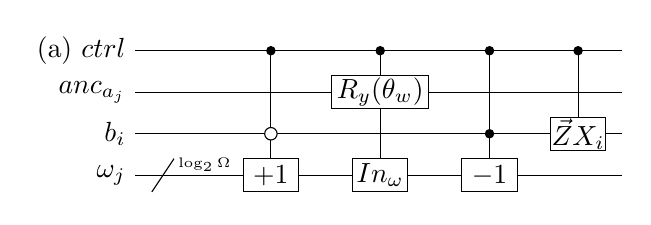
\begin{tikzpicture}[scale=1.000000,x=1pt,y=1pt]
\filldraw[color=white] (0.000000, -7.500000) rectangle (176.000000, 52.500000);
% Drawing wires
% Line 1: ctrl W \text{(a) }ctrl
\draw[color=black] (0.000000,45.000000) -- (176.000000,45.000000);
\draw[color=black] (0.000000,45.000000) node[left] {$\text{(a) }ctrl$};
% Line 2: anc_a W anc_{a_j}
\draw[color=black] (0.000000,30.000000) -- (176.000000,30.000000);
\draw[color=black] (0.000000,30.000000) node[left] {$anc_{a_j}$};
% Line 3: i W b_i
\draw[color=black] (0.000000,15.000000) -- (176.000000,15.000000);
\draw[color=black] (0.000000,15.000000) node[left] {$b_i$};
% Line 4: j W \omega_j
\draw[color=black] (0.000000,0.000000) -- (176.000000,0.000000);
\draw[color=black] (0.000000,0.000000) node[left] {$\omega_j$};
% Done with wires; drawing gates
% Line 6: j / ^{\log_2{\Omega}}
\draw (6.000000, -6.000000) -- (14.000000, 6.000000);
\draw (12.000000, 3.000000) node[right] {$\scriptstyle{^{\log_2{\Omega}}}$};
% Line 7: ctrl i anc_a j LABEL width=1
% Line 9: j G width=20 $+1$ ctrl -i
\draw (49.000000,45.000000) -- (49.000000,0.000000);
\begin{scope}
\draw[fill=white] (49.000000, -0.000000) +(-45.000000:14.142136pt and 8.485281pt) -- +(45.000000:14.142136pt and 8.485281pt) -- +(135.000000:14.142136pt and 8.485281pt) -- +(225.000000:14.142136pt and 8.485281pt) -- cycle;
\clip (49.000000, -0.000000) +(-45.000000:14.142136pt and 8.485281pt) -- +(45.000000:14.142136pt and 8.485281pt) -- +(135.000000:14.142136pt and 8.485281pt) -- +(225.000000:14.142136pt and 8.485281pt) -- cycle;
\draw (49.000000, -0.000000) node {$+1$};
\end{scope}
\filldraw (49.000000, 45.000000) circle(1.500000pt);
\draw[fill=white] (49.000000, 15.000000) circle(2.250000pt);
% Line 10: anc_a G:width=35 $R_y(\theta_w)$ j G:width=20 $In_\omega$ ctrl
\draw (88.500000,45.000000) -- (88.500000,0.000000);
\begin{scope}
\draw[fill=white] (88.500000, 30.000000) +(-45.000000:24.748737pt and 8.485281pt) -- +(45.000000:24.748737pt and 8.485281pt) -- +(135.000000:24.748737pt and 8.485281pt) -- +(225.000000:24.748737pt and 8.485281pt) -- cycle;
\clip (88.500000, 30.000000) +(-45.000000:24.748737pt and 8.485281pt) -- +(45.000000:24.748737pt and 8.485281pt) -- +(135.000000:24.748737pt and 8.485281pt) -- +(225.000000:24.748737pt and 8.485281pt) -- cycle;
\draw (88.500000, 30.000000) node {$R_y(\theta_w)$};
\end{scope}
\begin{scope}
\draw[fill=white] (88.500000, -0.000000) +(-45.000000:14.142136pt and 8.485281pt) -- +(45.000000:14.142136pt and 8.485281pt) -- +(135.000000:14.142136pt and 8.485281pt) -- +(225.000000:14.142136pt and 8.485281pt) -- cycle;
\clip (88.500000, -0.000000) +(-45.000000:14.142136pt and 8.485281pt) -- +(45.000000:14.142136pt and 8.485281pt) -- +(135.000000:14.142136pt and 8.485281pt) -- +(225.000000:14.142136pt and 8.485281pt) -- cycle;
\draw (88.500000, -0.000000) node {$In_\omega$};
\end{scope}
\filldraw (88.500000, 45.000000) circle(1.500000pt);
% Line 11: j G width=20 $-1$ ctrl i
\draw (128.000000,45.000000) -- (128.000000,0.000000);
\begin{scope}
\draw[fill=white] (128.000000, -0.000000) +(-45.000000:14.142136pt and 8.485281pt) -- +(45.000000:14.142136pt and 8.485281pt) -- +(135.000000:14.142136pt and 8.485281pt) -- +(225.000000:14.142136pt and 8.485281pt) -- cycle;
\clip (128.000000, -0.000000) +(-45.000000:14.142136pt and 8.485281pt) -- +(45.000000:14.142136pt and 8.485281pt) -- +(135.000000:14.142136pt and 8.485281pt) -- +(225.000000:14.142136pt and 8.485281pt) -- cycle;
\draw (128.000000, -0.000000) node {$-1$};
\end{scope}
\filldraw (128.000000, 45.000000) circle(1.500000pt);
\filldraw (128.000000, 15.000000) circle(1.500000pt);
% Line 13: i G width=20 $\vec{Z}X_i$ ctrl
\draw (160.000000,45.000000) -- (160.000000,15.000000);
\begin{scope}
\draw[fill=white] (160.000000, 15.000000) +(-45.000000:14.142136pt and 8.485281pt) -- +(45.000000:14.142136pt and 8.485281pt) -- +(135.000000:14.142136pt and 8.485281pt) -- +(225.000000:14.142136pt and 8.485281pt) -- cycle;
\clip (160.000000, 15.000000) +(-45.000000:14.142136pt and 8.485281pt) -- +(45.000000:14.142136pt and 8.485281pt) -- +(135.000000:14.142136pt and 8.485281pt) -- +(225.000000:14.142136pt and 8.485281pt) -- cycle;
\draw (160.000000, 15.000000) node {$\vec{Z}X_i$};
\end{scope}
\filldraw (160.000000, 45.000000) circle(1.500000pt);
% Done with gates; drawing ending labels
% Done with ending labels; drawing cut lines and comments
% Done with comments
\end{tikzpicture}

    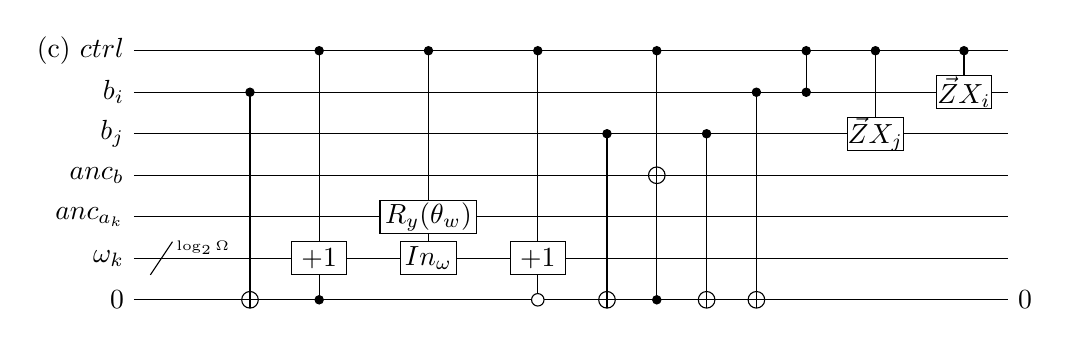
\begin{tikzpicture}[scale=1.000000,x=1pt,y=1pt]
\filldraw[color=white] (0.000000, -7.500000) rectangle (316.000000, 97.500000);
% Drawing wires
% Line 1: ctrl W \text{(c) }ctrl
\draw[color=black] (0.000000,90.000000) -- (316.000000,90.000000);
\draw[color=black] (0.000000,90.000000) node[left] {$\text{(c) }ctrl$};
% Line 2: i W b_i
\draw[color=black] (0.000000,75.000000) -- (316.000000,75.000000);
\draw[color=black] (0.000000,75.000000) node[left] {$b_i$};
% Line 3: j W b_j
\draw[color=black] (0.000000,60.000000) -- (316.000000,60.000000);
\draw[color=black] (0.000000,60.000000) node[left] {$b_j$};
% Line 4: anc_b W anc_b
\draw[color=black] (0.000000,45.000000) -- (316.000000,45.000000);
\draw[color=black] (0.000000,45.000000) node[left] {$anc_b$};
% Line 5: anc_a W anc_{a_k}
\draw[color=black] (0.000000,30.000000) -- (316.000000,30.000000);
\draw[color=black] (0.000000,30.000000) node[left] {$anc_{a_k}$};
% Line 6: k W \omega_k
\draw[color=black] (0.000000,15.000000) -- (316.000000,15.000000);
\draw[color=black] (0.000000,15.000000) node[left] {$\omega_k$};
% Line 7: c0 W 0 0
\draw[color=black] (0.000000,0.000000) -- (316.000000,0.000000);
\draw[color=black] (0.000000,0.000000) node[left] {$0$};
% Done with wires; drawing gates
% Line 9: k / ^{\log_2{\Omega}}
\draw (6.000000, 9.000000) -- (14.000000, 21.000000);
\draw (12.000000, 18.000000) node[right] {$\scriptstyle{^{\log_2{\Omega}}}$};
% Line 10: ctrl i j anc_b anc_a k c0 LABEL width=1
% Line 12: i +c0
\draw (42.000000,75.000000) -- (42.000000,0.000000);
\filldraw (42.000000, 75.000000) circle(1.500000pt);
\begin{scope}
\draw[fill=white] (42.000000, 0.000000) circle(3.000000pt);
\clip (42.000000, 0.000000) circle(3.000000pt);
\draw (39.000000, 0.000000) -- (45.000000, 0.000000);
\draw (42.000000, -3.000000) -- (42.000000, 3.000000);
\end{scope}
% Line 13: k G width=20 $+1$ ctrl c0
\draw (67.000000,90.000000) -- (67.000000,0.000000);
\begin{scope}
\draw[fill=white] (67.000000, 15.000000) +(-45.000000:14.142136pt and 8.485281pt) -- +(45.000000:14.142136pt and 8.485281pt) -- +(135.000000:14.142136pt and 8.485281pt) -- +(225.000000:14.142136pt and 8.485281pt) -- cycle;
\clip (67.000000, 15.000000) +(-45.000000:14.142136pt and 8.485281pt) -- +(45.000000:14.142136pt and 8.485281pt) -- +(135.000000:14.142136pt and 8.485281pt) -- +(225.000000:14.142136pt and 8.485281pt) -- cycle;
\draw (67.000000, 15.000000) node {$+1$};
\end{scope}
\filldraw (67.000000, 90.000000) circle(1.500000pt);
\filldraw (67.000000, 0.000000) circle(1.500000pt);
% Line 14: anc_a G:width=35 $R_y(\theta_w)$ k G:width=20 $In_\omega$ ctrl
\draw (106.500000,90.000000) -- (106.500000,15.000000);
\begin{scope}
\draw[fill=white] (106.500000, 30.000000) +(-45.000000:24.748737pt and 8.485281pt) -- +(45.000000:24.748737pt and 8.485281pt) -- +(135.000000:24.748737pt and 8.485281pt) -- +(225.000000:24.748737pt and 8.485281pt) -- cycle;
\clip (106.500000, 30.000000) +(-45.000000:24.748737pt and 8.485281pt) -- +(45.000000:24.748737pt and 8.485281pt) -- +(135.000000:24.748737pt and 8.485281pt) -- +(225.000000:24.748737pt and 8.485281pt) -- cycle;
\draw (106.500000, 30.000000) node {$R_y(\theta_w)$};
\end{scope}
\begin{scope}
\draw[fill=white] (106.500000, 15.000000) +(-45.000000:14.142136pt and 8.485281pt) -- +(45.000000:14.142136pt and 8.485281pt) -- +(135.000000:14.142136pt and 8.485281pt) -- +(225.000000:14.142136pt and 8.485281pt) -- cycle;
\clip (106.500000, 15.000000) +(-45.000000:14.142136pt and 8.485281pt) -- +(45.000000:14.142136pt and 8.485281pt) -- +(135.000000:14.142136pt and 8.485281pt) -- +(225.000000:14.142136pt and 8.485281pt) -- cycle;
\draw (106.500000, 15.000000) node {$In_\omega$};
\end{scope}
\filldraw (106.500000, 90.000000) circle(1.500000pt);
% Line 15: k G width=20 $+1$ ctrl -c0
\draw (146.000000,90.000000) -- (146.000000,0.000000);
\begin{scope}
\draw[fill=white] (146.000000, 15.000000) +(-45.000000:14.142136pt and 8.485281pt) -- +(45.000000:14.142136pt and 8.485281pt) -- +(135.000000:14.142136pt and 8.485281pt) -- +(225.000000:14.142136pt and 8.485281pt) -- cycle;
\clip (146.000000, 15.000000) +(-45.000000:14.142136pt and 8.485281pt) -- +(45.000000:14.142136pt and 8.485281pt) -- +(135.000000:14.142136pt and 8.485281pt) -- +(225.000000:14.142136pt and 8.485281pt) -- cycle;
\draw (146.000000, 15.000000) node {$+1$};
\end{scope}
\filldraw (146.000000, 90.000000) circle(1.500000pt);
\draw[fill=white] (146.000000, 0.000000) circle(2.250000pt);
% Line 16: j +c0
\draw (171.000000,60.000000) -- (171.000000,0.000000);
\filldraw (171.000000, 60.000000) circle(1.500000pt);
\begin{scope}
\draw[fill=white] (171.000000, 0.000000) circle(3.000000pt);
\clip (171.000000, 0.000000) circle(3.000000pt);
\draw (168.000000, 0.000000) -- (174.000000, 0.000000);
\draw (171.000000, -3.000000) -- (171.000000, 3.000000);
\end{scope}
% Line 18: ctrl c0 +anc_b
\draw (189.000000,90.000000) -- (189.000000,0.000000);
\filldraw (189.000000, 90.000000) circle(1.500000pt);
\filldraw (189.000000, 0.000000) circle(1.500000pt);
\begin{scope}
\draw[fill=white] (189.000000, 45.000000) circle(3.000000pt);
\clip (189.000000, 45.000000) circle(3.000000pt);
\draw (186.000000, 45.000000) -- (192.000000, 45.000000);
\draw (189.000000, 42.000000) -- (189.000000, 48.000000);
\end{scope}
% Line 19: j +c0
\draw (207.000000,60.000000) -- (207.000000,0.000000);
\filldraw (207.000000, 60.000000) circle(1.500000pt);
\begin{scope}
\draw[fill=white] (207.000000, 0.000000) circle(3.000000pt);
\clip (207.000000, 0.000000) circle(3.000000pt);
\draw (204.000000, 0.000000) -- (210.000000, 0.000000);
\draw (207.000000, -3.000000) -- (207.000000, 3.000000);
\end{scope}
% Line 20: i +c0
\draw (225.000000,75.000000) -- (225.000000,0.000000);
\filldraw (225.000000, 75.000000) circle(1.500000pt);
\begin{scope}
\draw[fill=white] (225.000000, 0.000000) circle(3.000000pt);
\clip (225.000000, 0.000000) circle(3.000000pt);
\draw (222.000000, 0.000000) -- (228.000000, 0.000000);
\draw (225.000000, -3.000000) -- (225.000000, 3.000000);
\end{scope}
% Line 22: ctrl i
\draw (243.000000,90.000000) -- (243.000000,75.000000);
\filldraw (243.000000, 90.000000) circle(1.500000pt);
\filldraw (243.000000, 75.000000) circle(1.500000pt);
% Line 24: j G width=20 $\vec{Z}X_j$ ctrl
\draw (268.000000,90.000000) -- (268.000000,60.000000);
\begin{scope}
\draw[fill=white] (268.000000, 60.000000) +(-45.000000:14.142136pt and 8.485281pt) -- +(45.000000:14.142136pt and 8.485281pt) -- +(135.000000:14.142136pt and 8.485281pt) -- +(225.000000:14.142136pt and 8.485281pt) -- cycle;
\clip (268.000000, 60.000000) +(-45.000000:14.142136pt and 8.485281pt) -- +(45.000000:14.142136pt and 8.485281pt) -- +(135.000000:14.142136pt and 8.485281pt) -- +(225.000000:14.142136pt and 8.485281pt) -- cycle;
\draw (268.000000, 60.000000) node {$\vec{Z}X_j$};
\end{scope}
\filldraw (268.000000, 90.000000) circle(1.500000pt);
% Line 25: i G width=20 $\vec{Z}X_i$ ctrl
\draw (300.000000,90.000000) -- (300.000000,75.000000);
\begin{scope}
\draw[fill=white] (300.000000, 75.000000) +(-45.000000:14.142136pt and 8.485281pt) -- +(45.000000:14.142136pt and 8.485281pt) -- +(135.000000:14.142136pt and 8.485281pt) -- +(225.000000:14.142136pt and 8.485281pt) -- cycle;
\clip (300.000000, 75.000000) +(-45.000000:14.142136pt and 8.485281pt) -- +(45.000000:14.142136pt and 8.485281pt) -- +(135.000000:14.142136pt and 8.485281pt) -- +(225.000000:14.142136pt and 8.485281pt) -- cycle;
\draw (300.000000, 75.000000) node {$\vec{Z}X_i$};
\end{scope}
\filldraw (300.000000, 90.000000) circle(1.500000pt);
% Done with gates; drawing ending labels
\draw[color=black] (316.000000,0.000000) node[right] {$0$};
% Done with ending labels; drawing cut lines and comments
% Done with comments
\end{tikzpicture}

    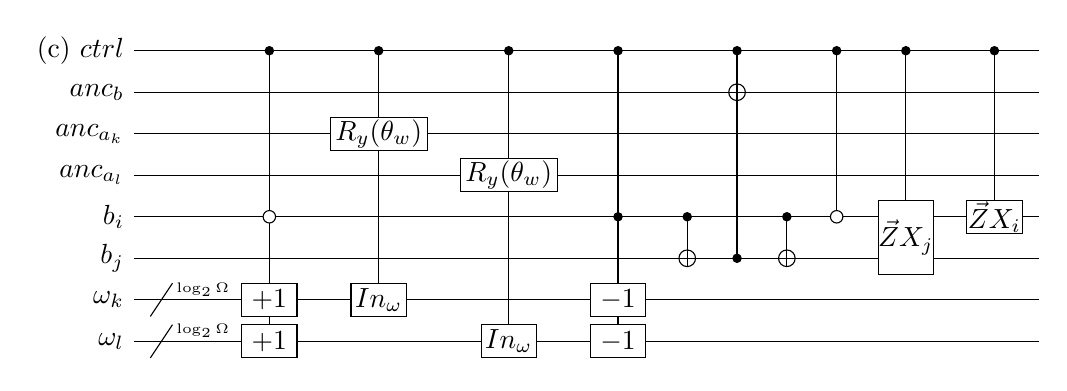
\begin{tikzpicture}[scale=1.000000,x=1pt,y=1pt]
\filldraw[color=white] (0.000000, -7.500000) rectangle (327.000000, 112.500000);
% Drawing wires
% Line 1: ctrl W \text{(c) }ctrl
\draw[color=black] (0.000000,105.000000) -- (327.000000,105.000000);
\draw[color=black] (0.000000,105.000000) node[left] {$\text{(c) }ctrl$};
% Line 2: anc_b W anc_b
\draw[color=black] (0.000000,90.000000) -- (327.000000,90.000000);
\draw[color=black] (0.000000,90.000000) node[left] {$anc_b$};
% Line 3: anc_k W anc_{a_k}
\draw[color=black] (0.000000,75.000000) -- (327.000000,75.000000);
\draw[color=black] (0.000000,75.000000) node[left] {$anc_{a_k}$};
% Line 4: anc_l W anc_{a_l}
\draw[color=black] (0.000000,60.000000) -- (327.000000,60.000000);
\draw[color=black] (0.000000,60.000000) node[left] {$anc_{a_l}$};
% Line 5: i W b_i
\draw[color=black] (0.000000,45.000000) -- (327.000000,45.000000);
\draw[color=black] (0.000000,45.000000) node[left] {$b_i$};
% Line 6: j W b_j
\draw[color=black] (0.000000,30.000000) -- (327.000000,30.000000);
\draw[color=black] (0.000000,30.000000) node[left] {$b_j$};
% Line 7: k W \omega_k
\draw[color=black] (0.000000,15.000000) -- (327.000000,15.000000);
\draw[color=black] (0.000000,15.000000) node[left] {$\omega_k$};
% Line 8: l W \omega_l
\draw[color=black] (0.000000,0.000000) -- (327.000000,0.000000);
\draw[color=black] (0.000000,0.000000) node[left] {$\omega_l$};
% Done with wires; drawing gates
% Line 10: k / ^{\log_2{\Omega}}
\draw (6.000000, 9.000000) -- (14.000000, 21.000000);
\draw (12.000000, 18.000000) node[right] {$\scriptstyle{^{\log_2{\Omega}}}$};
% Line 11: l / ^{\log_2{\Omega}}
\draw (6.000000, -6.000000) -- (14.000000, 6.000000);
\draw (12.000000, 3.000000) node[right] {$\scriptstyle{^{\log_2{\Omega}}}$};
% Line 12: ctrl i j anc_b anc_k anc_l k l LABEL width=1
% Line 14: k G width=20 $+1$ l G width=20 $+1$ ctrl -i
\draw (49.000000,105.000000) -- (49.000000,0.000000);
\begin{scope}
\draw[fill=white] (49.000000, 15.000000) +(-45.000000:14.142136pt and 8.485281pt) -- +(45.000000:14.142136pt and 8.485281pt) -- +(135.000000:14.142136pt and 8.485281pt) -- +(225.000000:14.142136pt and 8.485281pt) -- cycle;
\clip (49.000000, 15.000000) +(-45.000000:14.142136pt and 8.485281pt) -- +(45.000000:14.142136pt and 8.485281pt) -- +(135.000000:14.142136pt and 8.485281pt) -- +(225.000000:14.142136pt and 8.485281pt) -- cycle;
\draw (49.000000, 15.000000) node {$+1$};
\end{scope}
\begin{scope}
\draw[fill=white] (49.000000, -0.000000) +(-45.000000:14.142136pt and 8.485281pt) -- +(45.000000:14.142136pt and 8.485281pt) -- +(135.000000:14.142136pt and 8.485281pt) -- +(225.000000:14.142136pt and 8.485281pt) -- cycle;
\clip (49.000000, -0.000000) +(-45.000000:14.142136pt and 8.485281pt) -- +(45.000000:14.142136pt and 8.485281pt) -- +(135.000000:14.142136pt and 8.485281pt) -- +(225.000000:14.142136pt and 8.485281pt) -- cycle;
\draw (49.000000, -0.000000) node {$+1$};
\end{scope}
\filldraw (49.000000, 105.000000) circle(1.500000pt);
\draw[fill=white] (49.000000, 45.000000) circle(2.250000pt);
% Line 15: anc_k G:width=35 $R_y(\theta_w)$ k G:width=20 $In_\omega$ ctrl
\draw (88.500000,105.000000) -- (88.500000,15.000000);
\begin{scope}
\draw[fill=white] (88.500000, 75.000000) +(-45.000000:24.748737pt and 8.485281pt) -- +(45.000000:24.748737pt and 8.485281pt) -- +(135.000000:24.748737pt and 8.485281pt) -- +(225.000000:24.748737pt and 8.485281pt) -- cycle;
\clip (88.500000, 75.000000) +(-45.000000:24.748737pt and 8.485281pt) -- +(45.000000:24.748737pt and 8.485281pt) -- +(135.000000:24.748737pt and 8.485281pt) -- +(225.000000:24.748737pt and 8.485281pt) -- cycle;
\draw (88.500000, 75.000000) node {$R_y(\theta_w)$};
\end{scope}
\begin{scope}
\draw[fill=white] (88.500000, 15.000000) +(-45.000000:14.142136pt and 8.485281pt) -- +(45.000000:14.142136pt and 8.485281pt) -- +(135.000000:14.142136pt and 8.485281pt) -- +(225.000000:14.142136pt and 8.485281pt) -- cycle;
\clip (88.500000, 15.000000) +(-45.000000:14.142136pt and 8.485281pt) -- +(45.000000:14.142136pt and 8.485281pt) -- +(135.000000:14.142136pt and 8.485281pt) -- +(225.000000:14.142136pt and 8.485281pt) -- cycle;
\draw (88.500000, 15.000000) node {$In_\omega$};
\end{scope}
\filldraw (88.500000, 105.000000) circle(1.500000pt);
% Line 16: anc_l G:width=35 $R_y(\theta_w)$ l G:width=20 $In_\omega$ ctrl
\draw (135.500000,105.000000) -- (135.500000,0.000000);
\begin{scope}
\draw[fill=white] (135.500000, 60.000000) +(-45.000000:24.748737pt and 8.485281pt) -- +(45.000000:24.748737pt and 8.485281pt) -- +(135.000000:24.748737pt and 8.485281pt) -- +(225.000000:24.748737pt and 8.485281pt) -- cycle;
\clip (135.500000, 60.000000) +(-45.000000:24.748737pt and 8.485281pt) -- +(45.000000:24.748737pt and 8.485281pt) -- +(135.000000:24.748737pt and 8.485281pt) -- +(225.000000:24.748737pt and 8.485281pt) -- cycle;
\draw (135.500000, 60.000000) node {$R_y(\theta_w)$};
\end{scope}
\begin{scope}
\draw[fill=white] (135.500000, -0.000000) +(-45.000000:14.142136pt and 8.485281pt) -- +(45.000000:14.142136pt and 8.485281pt) -- +(135.000000:14.142136pt and 8.485281pt) -- +(225.000000:14.142136pt and 8.485281pt) -- cycle;
\clip (135.500000, -0.000000) +(-45.000000:14.142136pt and 8.485281pt) -- +(45.000000:14.142136pt and 8.485281pt) -- +(135.000000:14.142136pt and 8.485281pt) -- +(225.000000:14.142136pt and 8.485281pt) -- cycle;
\draw (135.500000, -0.000000) node {$In_\omega$};
\end{scope}
\filldraw (135.500000, 105.000000) circle(1.500000pt);
% Line 17: k G width=20 $-1$ l G width=20 $-1$ ctrl i
\draw (175.000000,105.000000) -- (175.000000,0.000000);
\begin{scope}
\draw[fill=white] (175.000000, 15.000000) +(-45.000000:14.142136pt and 8.485281pt) -- +(45.000000:14.142136pt and 8.485281pt) -- +(135.000000:14.142136pt and 8.485281pt) -- +(225.000000:14.142136pt and 8.485281pt) -- cycle;
\clip (175.000000, 15.000000) +(-45.000000:14.142136pt and 8.485281pt) -- +(45.000000:14.142136pt and 8.485281pt) -- +(135.000000:14.142136pt and 8.485281pt) -- +(225.000000:14.142136pt and 8.485281pt) -- cycle;
\draw (175.000000, 15.000000) node {$-1$};
\end{scope}
\begin{scope}
\draw[fill=white] (175.000000, -0.000000) +(-45.000000:14.142136pt and 8.485281pt) -- +(45.000000:14.142136pt and 8.485281pt) -- +(135.000000:14.142136pt and 8.485281pt) -- +(225.000000:14.142136pt and 8.485281pt) -- cycle;
\clip (175.000000, -0.000000) +(-45.000000:14.142136pt and 8.485281pt) -- +(45.000000:14.142136pt and 8.485281pt) -- +(135.000000:14.142136pt and 8.485281pt) -- +(225.000000:14.142136pt and 8.485281pt) -- cycle;
\draw (175.000000, -0.000000) node {$-1$};
\end{scope}
\filldraw (175.000000, 105.000000) circle(1.500000pt);
\filldraw (175.000000, 45.000000) circle(1.500000pt);
% Line 19: i +j
\draw (200.000000,45.000000) -- (200.000000,30.000000);
\filldraw (200.000000, 45.000000) circle(1.500000pt);
\begin{scope}
\draw[fill=white] (200.000000, 30.000000) circle(3.000000pt);
\clip (200.000000, 30.000000) circle(3.000000pt);
\draw (197.000000, 30.000000) -- (203.000000, 30.000000);
\draw (200.000000, 27.000000) -- (200.000000, 33.000000);
\end{scope}
% Line 20: ctrl j +anc_b
\draw (218.000000,105.000000) -- (218.000000,30.000000);
\filldraw (218.000000, 105.000000) circle(1.500000pt);
\filldraw (218.000000, 30.000000) circle(1.500000pt);
\begin{scope}
\draw[fill=white] (218.000000, 90.000000) circle(3.000000pt);
\clip (218.000000, 90.000000) circle(3.000000pt);
\draw (215.000000, 90.000000) -- (221.000000, 90.000000);
\draw (218.000000, 87.000000) -- (218.000000, 93.000000);
\end{scope}
% Line 21: i +j
\draw (236.000000,45.000000) -- (236.000000,30.000000);
\filldraw (236.000000, 45.000000) circle(1.500000pt);
\begin{scope}
\draw[fill=white] (236.000000, 30.000000) circle(3.000000pt);
\clip (236.000000, 30.000000) circle(3.000000pt);
\draw (233.000000, 30.000000) -- (239.000000, 30.000000);
\draw (236.000000, 27.000000) -- (236.000000, 33.000000);
\end{scope}
% Line 23: ctrl -i
\draw (254.000000,105.000000) -- (254.000000,45.000000);
\filldraw (254.000000, 105.000000) circle(1.500000pt);
\draw[fill=white] (254.000000, 45.000000) circle(2.250000pt);
% Line 25: i j G width=20 $\vec{Z}X_j$ ctrl
\draw (279.000000,105.000000) -- (279.000000,30.000000);
\begin{scope}
\draw[fill=white] (279.000000, 37.500000) +(-45.000000:14.142136pt and 19.091883pt) -- +(45.000000:14.142136pt and 19.091883pt) -- +(135.000000:14.142136pt and 19.091883pt) -- +(225.000000:14.142136pt and 19.091883pt) -- cycle;
\clip (279.000000, 37.500000) +(-45.000000:14.142136pt and 19.091883pt) -- +(45.000000:14.142136pt and 19.091883pt) -- +(135.000000:14.142136pt and 19.091883pt) -- +(225.000000:14.142136pt and 19.091883pt) -- cycle;
\draw (279.000000, 37.500000) node {$\vec{Z}X_j$};
\end{scope}
\filldraw (279.000000, 105.000000) circle(1.500000pt);
% Line 26: i G width=20 $\vec{Z}X_i$ ctrl
\draw (311.000000,105.000000) -- (311.000000,45.000000);
\begin{scope}
\draw[fill=white] (311.000000, 45.000000) +(-45.000000:14.142136pt and 8.485281pt) -- +(45.000000:14.142136pt and 8.485281pt) -- +(135.000000:14.142136pt and 8.485281pt) -- +(225.000000:14.142136pt and 8.485281pt) -- cycle;
\clip (311.000000, 45.000000) +(-45.000000:14.142136pt and 8.485281pt) -- +(45.000000:14.142136pt and 8.485281pt) -- +(135.000000:14.142136pt and 8.485281pt) -- +(225.000000:14.142136pt and 8.485281pt) -- cycle;
\draw (311.000000, 45.000000) node {$\vec{Z}X_i$};
\end{scope}
\filldraw (311.000000, 105.000000) circle(1.500000pt);
% Done with gates; drawing ending labels
% Done with ending labels; drawing cut lines and comments
% Done with comments
\end{tikzpicture}

    \caption{
        \textbf{Block-Encoding Terms}
        In subfigure (a), a block-encoding for the operator $b_i^\dagger a_j^\dagger + a_j b_i$ is given.
        In subfigure (b), a block-encoding for the operator $ b_i^\dagger b_j^\dagger a_k^\dagger + a_k b_j b_i$ is given.
        In subfigure (c), a block-encoding for the operator $b_i^\dagger b_j^\dagger a_k^\dagger a_l^\dagger + a_l a_k b_j b_i$ is given.
    }
    \label{fig:be-term-example}
\end{figure}


Consider the action of the operator: $b_i a_j + a_j^\dagger b_i^\dagger$ on the respective fermionic and bosonic modes.
When the fermionic mode is occupied, only the operator $b_i a_j$ will act nontrivially.
Meanwhile if the fermionic mode is unoccupied, only the operator $a_j^\dagger b_i^\dagger$ will act nontrivially.
Therefore, the occupation of the fermionic mode can be used to dictate which bosonic operator should be applied to the system.
After the appropriate bosonic operator is applied, the fermionic system is updated.
A circuit diagram for this block-encoding in given in subfigue \ref{fig:be-term-example}(a).
This block-encoding circuit will have a rescaling factor of $\lambda = \sqrt{\Omega}$, requires one block-encoding ancillae and $\lceil \log_2\Omega \rceil + 1$ clean ancillae, and uses $12 \lceil \Omega \rceil - 4$ T gates and (at most) $\Omega + 3$ arbitrary rotations.

This strategy can be employed for other combinations of bosonic and fermionic ladder operators.
In the full Yukawa model the operator $b_i^\dagger b_j^\dagger a_k^\dagger + a_k b_j b_i$ is used to model the process of a boson being annihilated to form a fermion and antifermion and a fermion and antifermion being annihilated to form a boson.
A block-encoding for this operator is shown in subfigue \ref{fig:be-term-example}(b).
When constructing the circuit, the occupation of either fermionic mode can be used to determine which bosonic operator is applied to the system.
This block-encoding circuit will have a rescaling factor of $\lambda = \sqrt{\Omega}$, requires two block-encoding ancillae and $\lceil \log_2\Omega \rceil + 1$ clean ancillae, and uses $12 \lceil \Omega \rceil$ T gates and (at most) $\Omega + 3$ arbitrary rotations.

A similar block-encoding can be constructed for the operator $b_i^\dagger b_j^\dagger a_k^\dagger a_l^\dagger + a_l a_k b_j b_i$, which appears in the full Yukawa model.
An example circuit diagram for this block-encoding is shown in subfigue \ref{fig:be-term-example}(c).
This block-encoding circuit will have a rescaling factor of $\lambda = \Omega$, requires three block-encoding ancillae and $\lceil \log_2\Omega \rceil + 1$ clean ancillae, and uses $24 \lceil \log_2\Omega \rceil - 8$ T gates and (at most) $2\Omega + 6$ arbitrary rotations.


\section{Results}
\label{sec:results}

In this section, we demonstrate the use of LOBE to block-encode physically-relevant Hamiltonians: the Yukawa and $\phi^4$ model used in \ws{insert-blah here @gus @kamil}.
We study both variants of the block-encoding described in Sections \ref{sec:block-encoding} and expanded upon in Section \ref{sec:lobe} and give numerical counts for the numbers of non-Clifford operations, the number of ancillae required beyond the system register, and the rescaling factor imposed on the resulting block-encoding.

\subsection{Yukawa Theory}
The most basic quantum field theory that describes interactions between bosons and fermions is Yukawa theory \cite{Schwartz_2013}. The interaction term is $\mathcal{L}_{\text{Yukawa}} = \bar\psi \psi \phi$, which leads to interaction vertices containing fermions and/or antifermions and bosons.

An auspicious coordinate system can be utilized called the lightfront frame \cite{Dirac1949}. In this frame, it is straightforward to write down the Hamiltonian bound state eigenvalue equation in terms of creation and annihilation operators, without the ambiguous $\sqrt{\nabla^2 + m^2}$ term that appears in a canonical instant-time frame Hamiltonian approach. 

The interaction terms in the Hamiltonian are $H_{\text{Yukawa int}} \in \{b^\dagger b a, b^\dagger b a^\dagger, d^\dagger d a, d^\dagger d a^\dagger, b^\dagger d^\dagger a, bda^\dagger, b^\dagger b a^\dagger a, d^\dagger d a^\dagger a \}$, while the free part of the Hamiltonian is $H_{\text{free}} \in \{b^\dagger b, d^\dagger d, a^\dagger a \}$.
This Hamiltonian can be written out as an integral (discretized to a sum in order to block encode with LOBE) over these free and interaction ladder operators modulated with coefficients (which are not added here). 


\begin{figure}
    \centering
    \includegraphics[width=16cm]{figures/Yukawa_hamiltonian_gates_vs_terms.pdf}
    \caption{
        \textbf{Numerical Gate Counts for Increasing $I$ (Yukawa Hamiltonian).}
        The number of rotations (left), left-elbows (middle), and right-elbows (right) are plotted as a function of the number of terms in the Hamiltonian ($L$) for an increasing number of momentum modes ($I$).
        The gate counts for the variant of LOBE using \textit{USP} are shown as the blue squares.
        The gate counts for the variant of LOBE using \textit{ASP} are shown as the orange circles.
        The bosonic occupancy cutoff ($\Omega$) is set to $3$.
        The number of rotations excludes rotations by angles that result in Clifford operations.
    }
    \label{fig:Yukawa_hamiltonian_gates_vs_terms}
\end{figure}
\begin{figure}
    \centering
    \includegraphics[width=12cm]{figures/Yukawa_hamiltonian_qubits_and_rescaling_vs_terms.pdf}
    \caption{
        \textbf{Numerical Ancillae Counts and Rescaling Factors for Increasing $I$ (Yukawa Hamiltonian).}
        The number of required ancillae (left) and the resulting rescaling factor (right) for LOBE are plotted as a function of the number of terms in the Hamiltonian ($L$) for an increasing number of momentum modes ($I$).
        The counts for the variant of LOBE using \textit{USP} are shown as the blue squares.
        The counts for the variant of LOBE using \textit{ASP} are shown as the orange circles.
        The bosonic occupancy cutoff ($\Omega$) is set to $3$.
    }
    \label{fig:Yukawa_hamiltonian_qubits_and_rescaling_vs_terms}
\end{figure}

In Figure \ref{fig:Yukawa_hamiltonian_gates_vs_terms}, we plot the numerical gate counts estimates for the Yukawa Hamiltonian (Eq. \ref{eq:Yukawa-hamiltonian}) \gus{@will do we want to explicitly show the discretized Hamiltonian for both Yukawa and $\phi^4$ in the appendix?} as the number of terms in the Hamiltonain ($L$) increases.
The number of terms ($L$) increases directly with an increasing number of momentum modes and is given by $L = 1.3I^3 + 0.65I^2 - 0.4I $ \ws{confirm this, im just eyeballing rn} \gus{I did some fits to $L$ vs. $I$, and got this from np.polyfit (see Yukawa.ipynb)}.
For the three non-Clifford operations, the number of operations increases linearly with the number of terms in the Hamiltonian for this model.
Additionally, the two different compilation strategies (\textit{USP} (blue), \textit{ASP} orange) demonstrate the same numerical scaling and have nearly identical gate counts for all types of operations.
When the number of terms ($L$) is far from the next largest power of 2, \textit{ASP} requires more arbitrary rotations due to the compilation of Grover-Rudolph that is used in this work.

In Figure \ref{fig:Yukawa_hamiltonian_qubits_and_rescaling_vs_terms}, we plot the numerical estimates for the number of required ancillae (left) and the imposed rescaling factor (right) as the number of terms in the Hamiltonain ($L$) increases.
The number of ancillae grows logarithmically with the number of terms for both implementations.
The number of ancillae used for the index register grows logarithmically with the number of terms which accounts for this scaling.
The main advantage of the \textit{ASP} variant is the effect on the rescaling factor of the block-encoding.
While the rescaling factor of both variants seemingly grows linearly with respect to the number of terms in the Hamiltonian, the rescaling factor for the \textit{ASP} variant is significantly smaller than the \textit{USP} variant.
When block-encodings are employed as a subroutine in larger algorithms, the quantum resources for the algorithm are often dependent on the rescaling factor (with a lower rescaling factor generally being preferred).
For example, in the context of using Quantum Phase Estimation to estimate the eigenvalues of a Hamiltonian, the number of gates required typically scales as $O(\frac{1}{\lambda})$ \cite{babbush2018encoding}. 
However, the exact cost associated with the rescaling factor is difficult to determine without choosing a specific algorithm to benchmark with.

\begin{figure}
    \centering
    \includegraphics[width=16cm]{figures/Yukawa_hamiltonian_gates_vs_omega.pdf}
    \caption{
        \textbf{Numerical Gate Counts for Increasing $\Omega$ (Yukawa Hamiltonian) .}
        The number of rotations (left), left-elbows (middle), and right-elbows (right) are plotted as a function of the bosonic occupation cutoff ($\Omega$).
        The gate counts for the variant of LOBE using \textit{USP} are shown as the blue squares.
        The gate counts for the variant of LOBE using \textit{ASP} are shown as the orange circles.
        The number of momentum modes ($I$) is set to $2$.
        The number of rotations excludes rotations by angles that result in Clifford operations.
    }
    \label{fig:Yukawa_hamiltonian_gates_vs_omega}
\end{figure}
\begin{figure}
    \centering
    \includegraphics[width=12cm]{figures/Yukawa_hamiltonian_qubits_and_rescaling_vs_omega.pdf}
    \caption{
        \textbf{Numerical Ancillae Counts and Rescaling Factors for Increasing $\Omega$ (Yukawa Hamiltonian).}
        The number of required ancillae (left) and the resulting rescaling factor (right) for LOBE are plotted as a function of the bosonic occupation cutoff ($\Omega$).
        The counts for the variant of LOBE using \textit{USP} are shown as the blue squares.
        The counts for the variant of LOBE using \textit{ASP} are shown as the orange circles.
        The number of momentum modes ($I$) is set to $2$.
    }
    \label{fig:Yukawa_hamiltonian_qubits_and_rescaling_vs_omega}
\end{figure}

In Figure \ref{fig:Yukawa_hamiltonian_gates_vs_omega}, we plot the numerical gate counts estimates for the Yukawa Hamiltonian (Eq. \ref{eq:Yukawa-hamiltonian}) as the cutoff on the maximum bosonic occupation ($\Omega$) increases.
For the three non-Clifford operations, the number of operations increases linearly with the bosonic occupancy cutoff for this model.
Similar to the case with increasing $I$, the two different compilation strategies (\textit{USP} (blue), \textit{ASP} orange) demonstrate the same numerical scaling and have nearly identical gate counts for all types of operations.

In Figure \ref{fig:Yukawa_hamiltonian_qubits_and_rescaling_vs_omega}, we plot the numerical estimates for the number of required ancillae (left) and the imposed rescaling factor (right) as the cutoff on the maximum bosonic occupation ($\Omega$) increases.
The number of ancillae grows logarithmically with the bosonic occupation cutoff for both implementations.
The number of ancillae needed to update the bosonic occupancy grows logarithmically with $\Omega$ (Eq. \ref{eq:ancillae-bosonic-updates}) which accounts for this scaling.
Again, the main advantage of the \textit{ASP} variant is that the imposed rescaling factor is significantly smaller than the \textit{USP} variant, especially for large values of $\Omega$ despite the asymptotic scaling being linear for both.


\subsection{$\phi^4$ Theory}
\gus{@kamil}
\input{text/results_qosc}
\input{text/results_static_yukawa}
\subsection{$\phi^4$ Results}
\label{sec:phi4_results}

The first interesting relativistic Hamiltonian studied with LOBE is $\phi^4$ theory. 
Any field theory is defined at the level of a Lagrangian, which for $\phi^4$ theory is given as
\begin{equation}
    \mathcal{L} = \frac12 \left(\partial_\mu \phi \right)^2 - \frac{m^2}{2}\phi^2 - g\phi^4.
\end{equation}

To obtain a Hamiltonian from a Lagrangian, a Legendre transformation is performed, in which an explicit set of coordinates must be chosen. 
The set of coordinates used in this paper, which lead to the simplest forms of the corresponding Hamiltonians, are front form (lightfront) coordinates \cite{Dirac1949}.
A discussion on lightfront coordinates, as well as the corresponding Hamiltonians for each theory studied will be given in appendix \ref{subsec:lightfront-hamiltonian}.

Unlike the non-relativistic theories, both relativistic theories are defined over many modes.
Thus, the results will be given as two sets of plots: one set of cost vs. \textit{resolution} (a discussion on resolution is given in the appendix. For those uninterested, this can be loosely thought of as number of modes), and one set of cost vs occupancy ($\Omega$.)

\begin{figure}[h]
    \centering
    \includegraphics[width = 15cm]{figures/phi4_resolutions.png}
    \caption{}
    \label{}
\end{figure}

\begin{figure}[h]
    \centering
    \includegraphics[width = 15cm]{figures/phi4_occupancies.png}
    \caption{}
    \label{}
\end{figure}
\input{text/results_full_yukawa}
\section{Conclusions}
\label{sec:conclusions}

In this work, we detail a framework which we refer to as LOBE (Ladder Operator Block-Encoding) which constructs block-encoding circuits for operators written in second-quantization.
We give explicit compilations for operators written as linear combinations of products of ladder operators acting on both fermionic and bosonic modes.
With this framework, many quantum operators of interest - such as Hamiltonians - can be block-encoded directly in their second-quantized form.
This avoids expanding operators in the Pauli basis prior to block-encoding which introduces a signficant overhead.

Additionally, we provide analytical and numerical costs for the relevant quantum resources required by LOBE for various operators of interest.
We compare our constructions to those that require the Jordan-Wigner and Standard Binary transformations to express ladder operators in the Pauli basis.
Our numerical results show that in most relevant cases, the LOBE framework produces block-encodings that require signficantly fewer T gates, non-Clifford rotations, block-encoding ancillae and total number of qubits and result in block-encodings with smaller rescaling factors.
In addition, the LOBE framework has better asymptotic scaling with respect to several parameters such as the maximum occupation of bosonic modes, the number of momentum modes, and the locality of the operator.
Notably, the LOBE constructions result in exponentially fewer non-Clifford operations for block-encoding products of ladder operators with respect to the locality as compared to a naive expansion of the operator in the Pauli basis.


\section{Acknowledgements}

Wop, wop, wop, wop, wop, Dot, fuck 'em up

Wop, wop, wop, wop, wop, I'ma do my stuff
\cite{Lamar_2024}

\bibliography{refs/citations}

\appendix

\section{Glossary}
\label{sec:glossary}

Here we explicitly define the technical phrases and symbols used throughout this work:

\begin{itemize}
    \item \textit{term} ($T$): An operator defined as a product of ladder operators.
    \item $L$: The number of terms in the Hamiltonian.
    \item $\Omega$: The occupation cutoff for the bosonic modes. $\Omega$ gives the maximum number of bosons that can be present in a single mode. 
    \item $I$: The number of momentum modes. The subscripts $b$, $d$, and $a$ will be used to denote the number of modes for a particular particle type.
    \item $b_i$: Fermionic annihilation (creation - $b_i^\dagger$) operator acting on mode $i$.
    \item $d_i$: Antifermionic annihilation (creation - $d_i^\dagger$) operator acting on mode $i$.
    \item $a_i$: Bosonic annihilation (creation - $a_i^\dagger$) operator acting on mode $i$.
    \item $n_{i_b}$: The number of fermions ($b$) occupying the $i^{th}$ mode. $n_{i_d}$ and $n_{i_a}$ give the occupancy for antifermions and bosons respectively.
    \item $B_l$: The number of fermionic modes with ladder operators acting on them within the term $T_l$.
    \item $D_l$: The number of antifermionic modes with ladder operators acting on them within the term $T_l$.
    \item $B$: The maximum number of fermionic \& antifermionic modes with ladder operators acting on them within a single term ($\max{b_l + d_l}$).
    \item $A_l$: The number of bosonic ladder operators within the term $T_l$. Operators raised to an exponent ($p$) count as $p$ operators.
    \item $A$: The maximum number of bosonic ladder operators acting within a single term ($\max_l A_l$). 
    \item $M_l$: The number of bosonic modes with ladder operators acting on them within the term $T_l$.
    \item $M$: The maximum number of bosonic modes with ladder operators acting on them within a single term ($\max_l M_l$).
    \item $S_{l, i}$: The exponent of bosonic annihilation operators acting on the $i^{th}$ bosonic mode within the $l^{th}$ term.
    \item $R_{l, i}$: The exponent of bosonic creation operators acting on the $i^{th}$ bosonic mode within the $l^{th}$ term.
    \item \textit{"zeroed-out"}: When the coefficient of a state becomes zero.
    \item \textit{encoded subspace}: The chosen subspace of the ancilla qubits used in the block-encoding to denote where the non-unitary operator is stored. Typically, this is the subspace where all ancillae are in the $\ket{0}$ state.
\end{itemize}
\section{Proof of $\lambda_{ASP} \leq \lambda_{USP}$}
\label{sec:proof-of-rescaling-factors}

\begin{theorem}
    $\lambda_{ASP} \leq \lambda_{USP}$
\end{theorem}

\textbf{Proof:} 

Define the following:
\begin{equation}
    \lambda_{USP} \equiv L\max_l|\tilde{\alpha}_l|
\end{equation}
and
\begin{equation}
    \lambda_{ASP} = \sum_l |\tilde{\alpha}_l|
\end{equation}

\textit{Case 1: All Coefficients are Equal}

Assume $\tilde{\alpha}_i = \tilde{\alpha}_j \forall i,j$.
Let $\tilde{\alpha}_i = \tilde{\alpha}$.
Then, $\lambda_{USP} \equiv L\max_l|\tilde{\alpha}_l| = L|\tilde{\alpha}|$ and $\sum_{l = 0}^{L - 1}|\tilde{\alpha}_l| = L|\tilde{\alpha}|$.
Thus, in this case, $\lambda_{USP} = \lambda_{ASP}$.

\textit{Case 2: Coefficients are Not All Equal}

Assume that there exist at least two coefficients, $\tilde{\alpha}_i$ and $\tilde{\alpha}_j$ such that $\tilde{\alpha}_i \neq \tilde{\alpha}_j$.
This implies that at least one coefficient, $\alpha_l$, has the largest magnitude.
Then, $\lambda_{ASP} = max_l|\tilde{\alpha}_l| + \sum_{k \neq l}|\tilde{\alpha}_k|$.
Now, if $\lambda_{ASP} < \lambda_{USP}$, then $\lambda_{ASP} - \lambda_{USP} < 0$:
\begin{align}
    \lambda_{ASP} - \lambda_{USP} &= max_l|\tilde{\alpha}_l| + \sum_{k \neq l}|\tilde{\alpha}_k| - Lmax_l|\tilde{\alpha}_l|\\ \nonumber
                                &= -(L - 1)max_l|\tilde{\alpha}_l|+ \sum_{k \neq l}|\tilde{\alpha}_k| \\ \nonumber
                                &< -(L - 1)max_l|\tilde{\alpha}_l| + \sum_{k \neq l}max_l|\tilde{\alpha}_l| \\ \nonumber
                                &= -(L - 1)max_l|\tilde{\alpha}_l| + (L - 1) max_l|\tilde{\alpha}_l|\\ \nonumber
                                &= 0 \\ \nonumber
\end{align}

Therefore, $\lambda_{ASP} \leq \lambda_{USP}$.$\blacksquare$

\section{Addition by a Known Classical Value}
\label{sec:addition}

Adding a (known) classical integer ($m$) to a quantum register encoded in binary is a required operation throughout this work:
\begin{equation}
    \label{eq:addition-by-classical-value}
    \ket{n} \rightarrow \ket{n + m}
\end{equation}
In an effort to keep this work self-contained and pedagogical, we review some methods for constructing this operation in this section.

\begin{figure}
    \centering
    \includegraphics[width=8cm]{figures/incrementer.pdf}
    \caption{
        \textbf{Controlled Incrementer} 
        A circuit diagram implementing a controlled incrementer (mod $32$) is shown.
        The controlled incrementer performs the operation $\ket{x} \rightarrow \ket{x + 1}$ when the control qubit is in the $\ket{1}$ state.
        Decrementing the register by $1$ can be achieved by applying Pauli-X gates on each qubit before and after the operation.
    }
    \label{fig:incrementer}
\end{figure}


One option is to use a series of controlled incrementer ($+1$) circuits.
An implementation of an incrementer circuit given by Gideny \cite{Gidney_2015} is shown in Figure \ref{fig:incrementer}.
If $N$ is the number of qubits in the register being incremented, this implementation requires $4(N-1)$ T gates and $N-1$ clean ancillae.
Naively, a series of $m$ incrementers will result in increasing the value of the register by $m \mod 2^N$.

\begin{figure}
    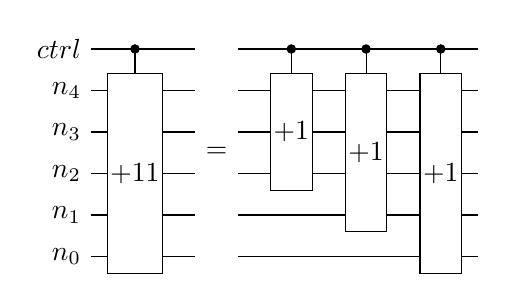
\begin{tikzpicture}[scale=1.000000,x=1pt,y=1pt]
\filldraw[color=white] (0.000000, -7.500000) rectangle (140.000000, 82.500000);
% Drawing wires
% Line 1: ctrl W ctrl
\draw[color=black] (0.000000,75.000000) -- (140.000000,75.000000);
\draw[color=black] (0.000000,75.000000) node[left] {$ctrl$};
% Line 2: n4 W n_4
\draw[color=black] (0.000000,60.000000) -- (140.000000,60.000000);
\draw[color=black] (0.000000,60.000000) node[left] {$n_4$};
% Line 3: n3 W n_3
\draw[color=black] (0.000000,45.000000) -- (140.000000,45.000000);
\draw[color=black] (0.000000,45.000000) node[left] {$n_3$};
% Line 4: n2 W n_2
\draw[color=black] (0.000000,30.000000) -- (140.000000,30.000000);
\draw[color=black] (0.000000,30.000000) node[left] {$n_2$};
% Line 5: n1 W n_1
\draw[color=black] (0.000000,15.000000) -- (140.000000,15.000000);
\draw[color=black] (0.000000,15.000000) node[left] {$n_1$};
% Line 6: n0 W n_0
\draw[color=black] (0.000000,0.000000) -- (140.000000,0.000000);
\draw[color=black] (0.000000,0.000000) node[left] {$n_0$};
% Done with wires; drawing gates
% Line 8: n4 n3 n2 n1 n0 G width=20 $+11$ ctrl
\draw (16.000000,75.000000) -- (16.000000,0.000000);
\begin{scope}
\draw[fill=white] (16.000000, 30.000000) +(-45.000000:14.142136pt and 50.911688pt) -- +(45.000000:14.142136pt and 50.911688pt) -- +(135.000000:14.142136pt and 50.911688pt) -- +(225.000000:14.142136pt and 50.911688pt) -- cycle;
\clip (16.000000, 30.000000) +(-45.000000:14.142136pt and 50.911688pt) -- +(45.000000:14.142136pt and 50.911688pt) -- +(135.000000:14.142136pt and 50.911688pt) -- +(225.000000:14.142136pt and 50.911688pt) -- cycle;
\draw (16.000000, 30.000000) node {$+11$};
\end{scope}
\filldraw (16.000000, 75.000000) circle(1.500000pt);
% Line 10: =
\draw[fill=white,color=white] (38.000000, -6.000000) rectangle (53.000000, 81.000000);
\draw (45.500000, 37.500000) node {$=$};
% Line 12: n4 n3 n2 G width=15 $+1$ ctrl
\draw (72.500000,75.000000) -- (72.500000,30.000000);
\begin{scope}
\draw[fill=white] (72.500000, 45.000000) +(-45.000000:10.606602pt and 29.698485pt) -- +(45.000000:10.606602pt and 29.698485pt) -- +(135.000000:10.606602pt and 29.698485pt) -- +(225.000000:10.606602pt and 29.698485pt) -- cycle;
\clip (72.500000, 45.000000) +(-45.000000:10.606602pt and 29.698485pt) -- +(45.000000:10.606602pt and 29.698485pt) -- +(135.000000:10.606602pt and 29.698485pt) -- +(225.000000:10.606602pt and 29.698485pt) -- cycle;
\draw (72.500000, 45.000000) node {$+1$};
\end{scope}
\filldraw (72.500000, 75.000000) circle(1.500000pt);
% Line 13: n4 n3 n2 n1 G width=15 $+1$ ctrl
\draw (99.500000,75.000000) -- (99.500000,15.000000);
\begin{scope}
\draw[fill=white] (99.500000, 37.500000) +(-45.000000:10.606602pt and 40.305087pt) -- +(45.000000:10.606602pt and 40.305087pt) -- +(135.000000:10.606602pt and 40.305087pt) -- +(225.000000:10.606602pt and 40.305087pt) -- cycle;
\clip (99.500000, 37.500000) +(-45.000000:10.606602pt and 40.305087pt) -- +(45.000000:10.606602pt and 40.305087pt) -- +(135.000000:10.606602pt and 40.305087pt) -- +(225.000000:10.606602pt and 40.305087pt) -- cycle;
\draw (99.500000, 37.500000) node {$+1$};
\end{scope}
\filldraw (99.500000, 75.000000) circle(1.500000pt);
% Line 14: n4 n3 n2 n1 n0 G width=15 $+1$ ctrl
\draw (126.500000,75.000000) -- (126.500000,0.000000);
\begin{scope}
\draw[fill=white] (126.500000, 30.000000) +(-45.000000:10.606602pt and 50.911688pt) -- +(45.000000:10.606602pt and 50.911688pt) -- +(135.000000:10.606602pt and 50.911688pt) -- +(225.000000:10.606602pt and 50.911688pt) -- cycle;
\clip (126.500000, 30.000000) +(-45.000000:10.606602pt and 50.911688pt) -- +(45.000000:10.606602pt and 50.911688pt) -- +(135.000000:10.606602pt and 50.911688pt) -- +(225.000000:10.606602pt and 50.911688pt) -- cycle;
\draw (126.500000, 30.000000) node {$+1$};
\end{scope}
\filldraw (126.500000, 75.000000) circle(1.500000pt);
% Done with gates; drawing ending labels
% Done with ending labels; drawing cut lines and comments
% Done with comments
\end{tikzpicture}

    \caption{
        \textbf{Addition via Incrementers} 
        An implementation of addition by a classical value ($11$) (mod $32$) using a series of incrementers is shown.
        An incrementer applied onto a register excluding the least-significant qubit implements a bit-shifted incrementer.
        This effectively increases the value of the register by $2$.
        Addition by the classical value $11$ can be constructed by bit-shifted incrementers adding the values $+8$, $+2$, and $+1$.
        Subtraction by the same value can be achieved by applying Pauli-X gates on each qubit before and after the operation.
    }
    \label{fig:addition-via-incrementers}
\end{figure}


However, an incrementer circuit can also be used to perform addition by a power of $2$ by acting on only the most-significant qubits.
For example, adding the value $8$ can be achieved using an incrementer circuit that treats the $4^{th}$ least significant qubit as the least significant qubit in the incrementer circuit and disregards the $3$ lesser qubits.
A circuit adding any classical value can then be constructed based on the binary representation of the classical number.
A circuit diagram for this construction is shown in Figure \ref{fig:addition-via-incrementers}.
The cost of this construction would require $N$ incrementer circuits requiring $4 \sum_{i=0}^{N - 2} N - i - 1$ T gates in total and $N - 1$ clean ancillae.

Since we are performing modular addition, the same result can also be achieved by subtracting the value $2^N - m$.
As an example, if the classical value is $31$ and $N = 5$, then this can be accomplished using a single decrementer circuit which can be constructed by conjugating an incrementer circuit with Pauli X gates acting on the qubits encoding $\ket{n}$.
The cost of these two methods can be classically determined and the more favorable option can be chosen during compilation.
The upper bound for the number of T gates, regardless of the classical value being added, is $N^2 + N$.
\ws{This scaling was determined numerically, but i think it shouldn't be hard to derive.}


\begin{figure}
    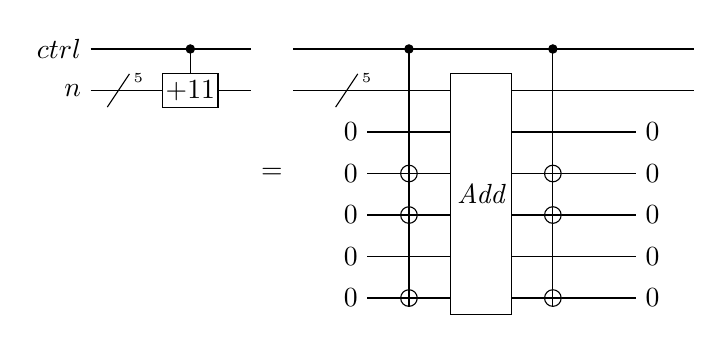
\begin{tikzpicture}[scale=1.000000,x=1pt,y=1pt]
\filldraw[color=white] (0.000000, -7.500000) rectangle (218.000000, 97.500000);
% Drawing wires
% Line 1: ctrl W ctrl
\draw[color=black] (0.000000,90.000000) -- (218.000000,90.000000);
\draw[color=black] (0.000000,90.000000) node[left] {$ctrl$};
% Line 2: n W n
\draw[color=black] (0.000000,75.000000) -- (218.000000,75.000000);
\draw[color=black] (0.000000,75.000000) node[left] {$n$};
% Line 3: m4 W 0 0
\draw[color=black] (92.500000,60.000000) -- (204.500000,60.000000);
% Line 4: m3 W 0 0
\draw[color=black] (92.500000,45.000000) -- (204.500000,45.000000);
% Line 5: m2 W 0 0
\draw[color=black] (92.500000,30.000000) -- (204.500000,30.000000);
% Line 6: m1 W 0 0
\draw[color=black] (92.500000,15.000000) -- (204.500000,15.000000);
% Line 7: m0 W 0 0
\draw[color=black] (92.500000,0.000000) -- (204.500000,0.000000);
% Done with wires; drawing gates
% Line 9: n / ^5
\draw (6.000000, 69.000000) -- (14.000000, 81.000000);
\draw (12.000000, 78.000000) node[right] {$\scriptstyle{^5}$};
% Line 11: n G width=20 $+11$ ctrl
\draw (36.000000,90.000000) -- (36.000000,75.000000);
\begin{scope}
\draw[fill=white] (36.000000, 75.000000) +(-45.000000:14.142136pt and 8.485281pt) -- +(45.000000:14.142136pt and 8.485281pt) -- +(135.000000:14.142136pt and 8.485281pt) -- +(225.000000:14.142136pt and 8.485281pt) -- cycle;
\clip (36.000000, 75.000000) +(-45.000000:14.142136pt and 8.485281pt) -- +(45.000000:14.142136pt and 8.485281pt) -- +(135.000000:14.142136pt and 8.485281pt) -- +(225.000000:14.142136pt and 8.485281pt) -- cycle;
\draw (36.000000, 75.000000) node {$+11$};
\end{scope}
\filldraw (36.000000, 90.000000) circle(1.500000pt);
% Line 13: =
\draw[fill=white,color=white] (58.000000, -6.000000) rectangle (73.000000, 96.000000);
\draw (65.500000, 45.000000) node {$=$};
% Line 15: n / ^5
\draw (88.500000, 69.000000) -- (96.500000, 81.000000);
\draw (94.500000, 78.000000) node[right] {$\scriptstyle{^5}$};
% Line 17: m4 START
\draw[color=black] (100.000000,60.000000) node[fill=white,left,minimum height=15.000000pt,minimum width=15.000000pt,inner sep=0pt] {\phantom{$0$}};
\draw[color=black] (100.000000,60.000000) node[left] {$0$};
% Line 18: m3 START
\draw[color=black] (100.000000,45.000000) node[fill=white,left,minimum height=15.000000pt,minimum width=15.000000pt,inner sep=0pt] {\phantom{$0$}};
\draw[color=black] (100.000000,45.000000) node[left] {$0$};
% Line 19: m2 START
\draw[color=black] (100.000000,30.000000) node[fill=white,left,minimum height=15.000000pt,minimum width=15.000000pt,inner sep=0pt] {\phantom{$0$}};
\draw[color=black] (100.000000,30.000000) node[left] {$0$};
% Line 20: m1 START
\draw[color=black] (100.000000,15.000000) node[fill=white,left,minimum height=15.000000pt,minimum width=15.000000pt,inner sep=0pt] {\phantom{$0$}};
\draw[color=black] (100.000000,15.000000) node[left] {$0$};
% Line 21: m0 START
\draw[color=black] (100.000000,0.000000) node[fill=white,left,minimum height=15.000000pt,minimum width=15.000000pt,inner sep=0pt] {\phantom{$0$}};
\draw[color=black] (100.000000,0.000000) node[left] {$0$};
% Line 22: ctrl +m3 +m2 +m0
\draw (115.000000,90.000000) -- (115.000000,0.000000);
\filldraw (115.000000, 90.000000) circle(1.500000pt);
\begin{scope}
\draw[fill=white] (115.000000, 45.000000) circle(3.000000pt);
\clip (115.000000, 45.000000) circle(3.000000pt);
\draw (112.000000, 45.000000) -- (118.000000, 45.000000);
\draw (115.000000, 42.000000) -- (115.000000, 48.000000);
\end{scope}
\begin{scope}
\draw[fill=white] (115.000000, 30.000000) circle(3.000000pt);
\clip (115.000000, 30.000000) circle(3.000000pt);
\draw (112.000000, 30.000000) -- (118.000000, 30.000000);
\draw (115.000000, 27.000000) -- (115.000000, 33.000000);
\end{scope}
\begin{scope}
\draw[fill=white] (115.000000, 0.000000) circle(3.000000pt);
\clip (115.000000, 0.000000) circle(3.000000pt);
\draw (112.000000, 0.000000) -- (118.000000, 0.000000);
\draw (115.000000, -3.000000) -- (115.000000, 3.000000);
\end{scope}
% Line 23: n m4 m3 m2 m1 m0 G width=22 $\textit{Add}$
\draw (141.000000,75.000000) -- (141.000000,0.000000);
\begin{scope}
\draw[fill=white] (141.000000, 37.500000) +(-45.000000:15.556349pt and 61.518290pt) -- +(45.000000:15.556349pt and 61.518290pt) -- +(135.000000:15.556349pt and 61.518290pt) -- +(225.000000:15.556349pt and 61.518290pt) -- cycle;
\clip (141.000000, 37.500000) +(-45.000000:15.556349pt and 61.518290pt) -- +(45.000000:15.556349pt and 61.518290pt) -- +(135.000000:15.556349pt and 61.518290pt) -- +(225.000000:15.556349pt and 61.518290pt) -- cycle;
\draw (141.000000, 37.500000) node {$\textit{Add}$};
\end{scope}
% Line 24: ctrl +m3 +m2 +m0
\draw (167.000000,90.000000) -- (167.000000,0.000000);
\filldraw (167.000000, 90.000000) circle(1.500000pt);
\begin{scope}
\draw[fill=white] (167.000000, 45.000000) circle(3.000000pt);
\clip (167.000000, 45.000000) circle(3.000000pt);
\draw (164.000000, 45.000000) -- (170.000000, 45.000000);
\draw (167.000000, 42.000000) -- (167.000000, 48.000000);
\end{scope}
\begin{scope}
\draw[fill=white] (167.000000, 30.000000) circle(3.000000pt);
\clip (167.000000, 30.000000) circle(3.000000pt);
\draw (164.000000, 30.000000) -- (170.000000, 30.000000);
\draw (167.000000, 27.000000) -- (167.000000, 33.000000);
\end{scope}
\begin{scope}
\draw[fill=white] (167.000000, 0.000000) circle(3.000000pt);
\clip (167.000000, 0.000000) circle(3.000000pt);
\draw (164.000000, 0.000000) -- (170.000000, 0.000000);
\draw (167.000000, -3.000000) -- (167.000000, 3.000000);
\end{scope}
% Line 25: m4 LABEL
% Line 26: m4 END
\draw[color=black] (197.000000,60.000000) node[fill=white,right,minimum height=15.000000pt,minimum width=15.000000pt,inner sep=0pt] {\phantom{$0$}};
\draw[color=black] (197.000000,60.000000) node[right] {$0$};
% Line 27: m3 END
\draw[color=black] (197.000000,45.000000) node[fill=white,right,minimum height=15.000000pt,minimum width=15.000000pt,inner sep=0pt] {\phantom{$0$}};
\draw[color=black] (197.000000,45.000000) node[right] {$0$};
% Line 28: m2 END
\draw[color=black] (197.000000,30.000000) node[fill=white,right,minimum height=15.000000pt,minimum width=15.000000pt,inner sep=0pt] {\phantom{$0$}};
\draw[color=black] (197.000000,30.000000) node[right] {$0$};
% Line 29: m1 END
\draw[color=black] (197.000000,15.000000) node[fill=white,right,minimum height=15.000000pt,minimum width=15.000000pt,inner sep=0pt] {\phantom{$0$}};
\draw[color=black] (197.000000,15.000000) node[right] {$0$};
% Line 30: m0 END
\draw[color=black] (197.000000,0.000000) node[fill=white,right,minimum height=15.000000pt,minimum width=15.000000pt,inner sep=0pt] {\phantom{$0$}};
\draw[color=black] (197.000000,0.000000) node[right] {$0$};
% Done with gates; drawing ending labels
% Done with ending labels; drawing cut lines and comments
% Done with comments
\end{tikzpicture}

    \caption{
        \textbf{Time-Efficient Controlled Addition of $11$}
        Increasing the value of a quantum register by a known classical value can be implemented using clean ancillae and an uncontrolled quantum addition circuit.
        The known classical value is loaded into a clean ancilla register using a series of CNOT gates corresponding to the binary representation of the classical value.
        Then an uncontrolled quantum addition circuit is applied to the two registers.
        Finally, the loading of the classical value is uncomputed.
    }
    \label{fig:addition-gate-efficient}
\end{figure}

Another option is to first load the classical value into an clean ancilla register, controlled on the control qubit, perform \textit{uncontrolled} (modular) addition of the two quantum registers, then ``unload'' the classical value.
If the control is off, then the classical value is not loaded and the uncontrolled addition simply adds the value $0$ and leaves the original register unchanged.
An example diagram for this construction depicting adding the value $m = 11$ to a register with $N = 5$ qubits is shown in Figure \ref{fig:addition-gate-efficient}.

The loading (and unloading) of the classical value only requires CNOTs and therefore does not contribute any non-Clifford resouces, but it does require $N$ clean ancillae.
However, if the $p$ least significant bits of $m$ are zero, then only $N - p$ qubits are required to load $m$ and the $p$ least-significant qubits of $N$ can be omitted from the addition.
Uncontrolled addition of two registers can be performed using $4(N-1)$ T gates and $N - 1$ clean ancillae using the construction for addition shown in Figure 1 of \cite{gidney2018halving}.
Therefore, in total, this compilation will require $4(N - p - 1)$ T gates and $2(N - p) - 1$ clean ancillae.

When $m$ is a power of $2$, then compilation using incrementer circuits uses the same number of T gates, but fewer clean ancillae.
When $m$ is not a power of $2$, then the compilation using uncontrolled quantum addition uses fewer T gates (at the expense of more clean ancillae).
Since $m$ is known during compilation, an implementation can be chosen that results in the fewest required resources.

\begin{figure*}
    \centering
    \includegraphics[width=12cm]{figures/ctrl-add-11-qubit-efficient.pdf}
    \caption{
        \textbf{Space-Efficient Controlled Addition of 11}
        An implementation for increasing the value of a register by a known classical value is shown for the case when the known value is $11$ and the number of qubits in the register is $5$.
        The binary representation of $11$ is $01011$ with the left-most bit being the most-significant.
        The values of these $M$ classical bits can be propagated into the control structure of the controlled quantum addition.
        If the value of the $i^\text{th}$ bit of $M$ is $0$ ($1$), the corresponding control in the circuit is controlled on the $\ket{1}$  ($\ket{0}$) state.
    }
    \label{fig:addition-qubit-efficient-11}
\end{figure*}

\begin{figure}
    \centering
    \includegraphics[width=8cm]{figures/ctrl-add-12-qubit-efficient.pdf}
    \caption{
        \textbf{Space-Efficient Controlled Addition of 12} 
        An implementation for increasing the value of a register by a known classical value is shown for the case when the known value is $12$ ($01100$ in binary) and the number of qubits in the register is $5$.
        When the least-significant bits of $M$ are $0$, the circuit can be bit-shifted, resulting in a lower cost implementation.
        In this case, the two least-significant bits are $0$, so the circuit can be bit-shifted twice.
    }
    \label{fig:addition-qubit-efficient-12}
\end{figure}

Another implementation can be chosen to reduce the number of clean ancillae, which uses the classical information about $m$ to modify the circuit for \textit{controlled} quantum addition.
Controlled addition of two registers can be performed using $4(2N - 3)$ T gates and $2N - 1$ clean ancillae using the construction for addition shown in Figure 4 of \cite{gidney2018halving}.
This circuit can be modified by propagating the classical information about the binary encoding of $m$ into the control structure of the adder circuit, thereby reducing the number of clean ancillae by $N$.
An example diagram showing this propagation in the case where $m = 11$ and $N = 5$ is shown in Figure \ref{fig:addition-qubit-efficient-11}.

Similarly, if the $p$ least-significant bits of $m$ are known to be zero, the addition can be performed beginning with the first non-zero bit of $m$.
An example circuit diagram for the case where $m=12$ ($01100$ in binary) and $N = 5$ is shown in Figure \ref{fig:addition-qubit-efficient-12}.
If the $p$ least significant bits of $m$ are zero, then this circuit uses $4(2(N - p) - 3)$ T gates and $N - p - 1$ clean ancillae.
Since this work primarily focuses on reducing the number of T gates, the quantum resource estimates quoted in this work do not utilize this strategy.

\section{Standard Binary Bosonic Encoding}
\label{sec:SB}

An explicit encoding must be chosen to map bosonic ladder operators to qubit operators.
This is necessary to construct LCU circuits of the Hamiltonians in section \ref{sec:results}.
The encoding chosen matches the encoding of LOBE circuits is the standard binary \cite{standard-binary} encoding.

The encoding starts by noting that 

\begin{align}
    a^\dagger &= \sum_{s = 0}^{\Omega - 1}\sqrt{s + 1}|s + 1\rangle \langle s| = \ket{1}\bra{0} + \sqrt{2}\ket{2}\bra{1} + \dots\\
    a &= \sum_{s = 0}^{\Omega - 1}\sqrt{s + 1}|s\rangle \langle s + 1| = \ket{0}\bra{1} + \sqrt{2}\ket{1}\bra{2} + \dots\\
\end{align}

From here, each state in the expansion of $a, a^\dagger$ is converted into binary, e.g. $|3\rangle = |...11\rangle$, where the $\dots$ are zeros depending on $\Omega$.
Now, at each qubit index, the outer product can be computed by computing the outer product of the zeros and ones tensored together.
For example, take $\Omega = 3$,$$
\ket{2}\bra{3} = \ket{10}\bra{11} = \ket{1}\bra{1} \otimes \ket{0}\bra{1}.
$$
The last step is to work out the following outer products by noting that:

\begin{align}
    \ket{0}\bra{0} &= \frac12 \left(I + Z \right)\\
    \ket{0}\bra{1} &= \frac12 \left(X + iY \right)\\
    \ket{1}\bra{0} &= \frac12 \left(X - iY \right)\\
    \ket{1}\bra{1} &= \frac12 \left(I - Z \right)\\ 
\end{align}

Thus, as an example, with $\Omega = 3$, 

\begin{align}
    a_0^\dagger \rightarrow &0.683IX -0.183 ZX - 0.683\mathrm{i} IY + 0.183\mathrm{i} ZY \\
    & +0.354 XX - 0.354\mathrm{i} YX + 0.354\mathrm{i} XY + 0.354 YY
\end{align}
\section{Uniformly Controlled Rotations}
\label{sec:multiplexed-rotations}

Implementing a series of uniformly controlled rotations is a common subroutine used in this work.
In this section, we discuss the cost and explicit circuit compilation for a series of uniformly controlled rotations around the same axis (but different angles) are applied on the same qubit:
\begin{equation}
    \sum_{l=0}^{L - 1} \ket{l} \ket{\phi} \rightarrow \sum_{l=0}^{L - 1} \ket{l} R_a (\alpha_l) \ket{\phi}
\end{equation}

Möttönen et. al \cite{mottonen2004transformation}, provide a construction for \textit{uncontrolled} uniformly controlled rotations.
This construction is only defined when the number of rotations ($L$) is explicitly a power of $2$, however, if fewer rotations are required, then this can be achieved by padding with zero-angle rotations.

In this construction, the rotation angles are classically preprocessed based on the Gray code (Eq. 3 of \cite{mottonen2004transformation}):
\begin{equation}
    \begin{bmatrix}
        \theta_{0} \\
        \theta_{1} \\
        \vdots \\
        \theta_{L - 1}
    \end{bmatrix} = M \begin{bmatrix}
        \alpha_{0} \\
        \alpha_{1} \\
        \vdots \\
        \alpha_{L - 1}
    \end{bmatrix}
\end{equation}
where $M$ is a matrix transformation defined by:
\begin{equation}
    M_{i, j} = L^{-1} (-1)^{b_{j} . g_{i}}
\end{equation}
where $b_j$ is the binary representation of the integer $j$, $g_i$ is the Gray code representation of the integer $i$, and $b_{j} . g_{i}$ is the bitwise inner product of $b_{j}$ and $g_{i}$.

\begin{figure*}
    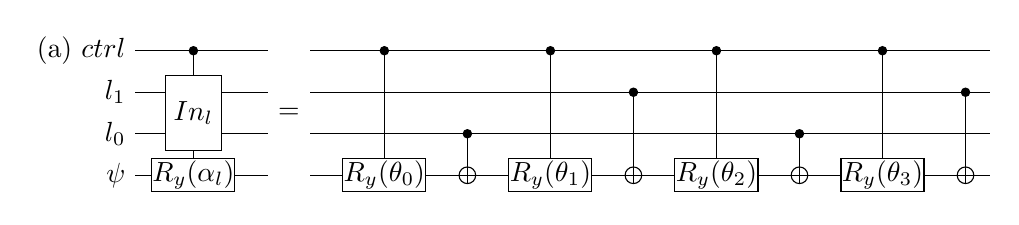
\begin{tikzpicture}[scale=1.000000,x=1pt,y=1pt]
\filldraw[color=white] (0.000000, -7.500000) rectangle (309.000000, 52.500000);
% Drawing wires
% Line 1: ctrl W \text{(a) }ctrl
\draw[color=black] (0.000000,45.000000) -- (309.000000,45.000000);
\draw[color=black] (0.000000,45.000000) node[left] {$\text{(a) }ctrl$};
% Line 2: l1 W l_1
\draw[color=black] (0.000000,30.000000) -- (309.000000,30.000000);
\draw[color=black] (0.000000,30.000000) node[left] {$l_1$};
% Line 3: l0 W l_0
\draw[color=black] (0.000000,15.000000) -- (309.000000,15.000000);
\draw[color=black] (0.000000,15.000000) node[left] {$l_0$};
% Line 4: sys W \psi
\draw[color=black] (0.000000,0.000000) -- (309.000000,0.000000);
\draw[color=black] (0.000000,0.000000) node[left] {$\psi$};
% Done with wires; drawing gates
% Line 6: l1 l0 G:width=20 $In_l$ sys G:width=30 $R_y (\alpha_l)$ ctrl
\draw (21.000000,45.000000) -- (21.000000,0.000000);
\begin{scope}
\draw[fill=white] (21.000000, 22.500000) +(-45.000000:14.142136pt and 19.091883pt) -- +(45.000000:14.142136pt and 19.091883pt) -- +(135.000000:14.142136pt and 19.091883pt) -- +(225.000000:14.142136pt and 19.091883pt) -- cycle;
\clip (21.000000, 22.500000) +(-45.000000:14.142136pt and 19.091883pt) -- +(45.000000:14.142136pt and 19.091883pt) -- +(135.000000:14.142136pt and 19.091883pt) -- +(225.000000:14.142136pt and 19.091883pt) -- cycle;
\draw (21.000000, 22.500000) node {$In_l$};
\end{scope}
\begin{scope}
\draw[fill=white] (21.000000, -0.000000) +(-45.000000:21.213203pt and 8.485281pt) -- +(45.000000:21.213203pt and 8.485281pt) -- +(135.000000:21.213203pt and 8.485281pt) -- +(225.000000:21.213203pt and 8.485281pt) -- cycle;
\clip (21.000000, -0.000000) +(-45.000000:21.213203pt and 8.485281pt) -- +(45.000000:21.213203pt and 8.485281pt) -- +(135.000000:21.213203pt and 8.485281pt) -- +(225.000000:21.213203pt and 8.485281pt) -- cycle;
\draw (21.000000, -0.000000) node {$R_y (\alpha_l)$};
\end{scope}
\filldraw (21.000000, 45.000000) circle(1.500000pt);
% Line 8: =
\draw[fill=white,color=white] (48.000000, -6.000000) rectangle (63.000000, 51.000000);
\draw (55.500000, 22.500000) node {$=$};
% Line 10: sys G width=30 $R_y (\theta_0)$ ctrl
\draw (90.000000,45.000000) -- (90.000000,0.000000);
\begin{scope}
\draw[fill=white] (90.000000, -0.000000) +(-45.000000:21.213203pt and 8.485281pt) -- +(45.000000:21.213203pt and 8.485281pt) -- +(135.000000:21.213203pt and 8.485281pt) -- +(225.000000:21.213203pt and 8.485281pt) -- cycle;
\clip (90.000000, -0.000000) +(-45.000000:21.213203pt and 8.485281pt) -- +(45.000000:21.213203pt and 8.485281pt) -- +(135.000000:21.213203pt and 8.485281pt) -- +(225.000000:21.213203pt and 8.485281pt) -- cycle;
\draw (90.000000, -0.000000) node {$R_y (\theta_0)$};
\end{scope}
\filldraw (90.000000, 45.000000) circle(1.500000pt);
% Line 11: +sys l0
\draw (120.000000,15.000000) -- (120.000000,0.000000);
\begin{scope}
\draw[fill=white] (120.000000, 0.000000) circle(3.000000pt);
\clip (120.000000, 0.000000) circle(3.000000pt);
\draw (117.000000, 0.000000) -- (123.000000, 0.000000);
\draw (120.000000, -3.000000) -- (120.000000, 3.000000);
\end{scope}
\filldraw (120.000000, 15.000000) circle(1.500000pt);
% Line 12: sys G width=30 $R_y (\theta_1)$ ctrl
\draw (150.000000,45.000000) -- (150.000000,0.000000);
\begin{scope}
\draw[fill=white] (150.000000, -0.000000) +(-45.000000:21.213203pt and 8.485281pt) -- +(45.000000:21.213203pt and 8.485281pt) -- +(135.000000:21.213203pt and 8.485281pt) -- +(225.000000:21.213203pt and 8.485281pt) -- cycle;
\clip (150.000000, -0.000000) +(-45.000000:21.213203pt and 8.485281pt) -- +(45.000000:21.213203pt and 8.485281pt) -- +(135.000000:21.213203pt and 8.485281pt) -- +(225.000000:21.213203pt and 8.485281pt) -- cycle;
\draw (150.000000, -0.000000) node {$R_y (\theta_1)$};
\end{scope}
\filldraw (150.000000, 45.000000) circle(1.500000pt);
% Line 13: +sys l1
\draw (180.000000,30.000000) -- (180.000000,0.000000);
\begin{scope}
\draw[fill=white] (180.000000, 0.000000) circle(3.000000pt);
\clip (180.000000, 0.000000) circle(3.000000pt);
\draw (177.000000, 0.000000) -- (183.000000, 0.000000);
\draw (180.000000, -3.000000) -- (180.000000, 3.000000);
\end{scope}
\filldraw (180.000000, 30.000000) circle(1.500000pt);
% Line 14: sys G width=30 $R_y (\theta_2)$ ctrl
\draw (210.000000,45.000000) -- (210.000000,0.000000);
\begin{scope}
\draw[fill=white] (210.000000, -0.000000) +(-45.000000:21.213203pt and 8.485281pt) -- +(45.000000:21.213203pt and 8.485281pt) -- +(135.000000:21.213203pt and 8.485281pt) -- +(225.000000:21.213203pt and 8.485281pt) -- cycle;
\clip (210.000000, -0.000000) +(-45.000000:21.213203pt and 8.485281pt) -- +(45.000000:21.213203pt and 8.485281pt) -- +(135.000000:21.213203pt and 8.485281pt) -- +(225.000000:21.213203pt and 8.485281pt) -- cycle;
\draw (210.000000, -0.000000) node {$R_y (\theta_2)$};
\end{scope}
\filldraw (210.000000, 45.000000) circle(1.500000pt);
% Line 15: +sys l0
\draw (240.000000,15.000000) -- (240.000000,0.000000);
\begin{scope}
\draw[fill=white] (240.000000, 0.000000) circle(3.000000pt);
\clip (240.000000, 0.000000) circle(3.000000pt);
\draw (237.000000, 0.000000) -- (243.000000, 0.000000);
\draw (240.000000, -3.000000) -- (240.000000, 3.000000);
\end{scope}
\filldraw (240.000000, 15.000000) circle(1.500000pt);
% Line 16: sys G width=30 $R_y (\theta_3)$ ctrl
\draw (270.000000,45.000000) -- (270.000000,0.000000);
\begin{scope}
\draw[fill=white] (270.000000, -0.000000) +(-45.000000:21.213203pt and 8.485281pt) -- +(45.000000:21.213203pt and 8.485281pt) -- +(135.000000:21.213203pt and 8.485281pt) -- +(225.000000:21.213203pt and 8.485281pt) -- cycle;
\clip (270.000000, -0.000000) +(-45.000000:21.213203pt and 8.485281pt) -- +(45.000000:21.213203pt and 8.485281pt) -- +(135.000000:21.213203pt and 8.485281pt) -- +(225.000000:21.213203pt and 8.485281pt) -- cycle;
\draw (270.000000, -0.000000) node {$R_y (\theta_3)$};
\end{scope}
\filldraw (270.000000, 45.000000) circle(1.500000pt);
% Line 17: +sys l1
\draw (300.000000,30.000000) -- (300.000000,0.000000);
\begin{scope}
\draw[fill=white] (300.000000, 0.000000) circle(3.000000pt);
\clip (300.000000, 0.000000) circle(3.000000pt);
\draw (297.000000, 0.000000) -- (303.000000, 0.000000);
\draw (300.000000, -3.000000) -- (300.000000, 3.000000);
\end{scope}
\filldraw (300.000000, 30.000000) circle(1.500000pt);
% Done with gates; drawing ending labels
% Done with ending labels; drawing cut lines and comments
% Done with comments
\end{tikzpicture}

    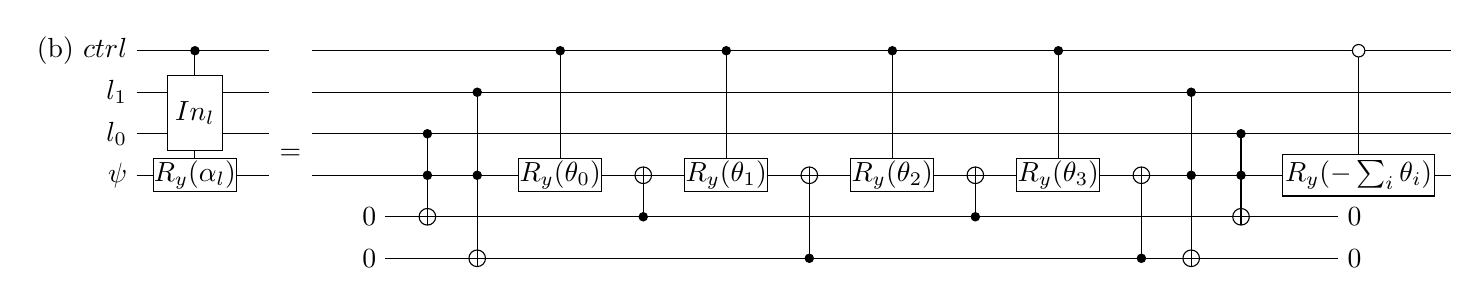
\begin{tikzpicture}[scale=1.000000,x=1pt,y=1pt]
\filldraw[color=white] (0.000000, -7.500000) rectangle (475.000000, 82.500000);
% Drawing wires
% Line 1: ctrl W \text{(b) }ctrl
\draw[color=black] (0.000000,75.000000) -- (475.000000,75.000000);
\draw[color=black] (0.000000,75.000000) node[left] {$\text{(b) }ctrl$};
% Line 2: l1 W l_1
\draw[color=black] (0.000000,60.000000) -- (475.000000,60.000000);
\draw[color=black] (0.000000,60.000000) node[left] {$l_1$};
% Line 3: l0 W l_0
\draw[color=black] (0.000000,45.000000) -- (475.000000,45.000000);
\draw[color=black] (0.000000,45.000000) node[left] {$l_0$};
% Line 4: sys W \psi
\draw[color=black] (0.000000,30.000000) -- (475.000000,30.000000);
\draw[color=black] (0.000000,30.000000) node[left] {$\psi$};
% Line 5: c0 W 0 0
\draw[color=black] (82.500000,15.000000) -- (441.500000,15.000000);
% Line 6: c1 W 0 0
\draw[color=black] (82.500000,0.000000) -- (441.500000,0.000000);
% Done with wires; drawing gates
% Line 8: sys G:width=30 $R_y (\alpha_l)$ l1 l0 G:width=20 $In_l$ ctrl
\draw (21.000000,75.000000) -- (21.000000,30.000000);
\begin{scope}
\draw[fill=white] (21.000000, 30.000000) +(-45.000000:21.213203pt and 8.485281pt) -- +(45.000000:21.213203pt and 8.485281pt) -- +(135.000000:21.213203pt and 8.485281pt) -- +(225.000000:21.213203pt and 8.485281pt) -- cycle;
\clip (21.000000, 30.000000) +(-45.000000:21.213203pt and 8.485281pt) -- +(45.000000:21.213203pt and 8.485281pt) -- +(135.000000:21.213203pt and 8.485281pt) -- +(225.000000:21.213203pt and 8.485281pt) -- cycle;
\draw (21.000000, 30.000000) node {$R_y (\alpha_l)$};
\end{scope}
\begin{scope}
\draw[fill=white] (21.000000, 52.500000) +(-45.000000:14.142136pt and 19.091883pt) -- +(45.000000:14.142136pt and 19.091883pt) -- +(135.000000:14.142136pt and 19.091883pt) -- +(225.000000:14.142136pt and 19.091883pt) -- cycle;
\clip (21.000000, 52.500000) +(-45.000000:14.142136pt and 19.091883pt) -- +(45.000000:14.142136pt and 19.091883pt) -- +(135.000000:14.142136pt and 19.091883pt) -- +(225.000000:14.142136pt and 19.091883pt) -- cycle;
\draw (21.000000, 52.500000) node {$In_l$};
\end{scope}
\filldraw (21.000000, 75.000000) circle(1.500000pt);
% Line 10: =
\draw[fill=white,color=white] (48.000000, -6.000000) rectangle (63.000000, 81.000000);
\draw (55.500000, 37.500000) node {$=$};
% Line 12: c0 c1 START
\draw[color=black] (90.000000,15.000000) node[fill=white,left,minimum height=15.000000pt,minimum width=15.000000pt,inner sep=0pt] {\phantom{$0$}};
\draw[color=black] (90.000000,15.000000) node[left] {$0$};
\draw[color=black] (90.000000,0.000000) node[fill=white,left,minimum height=15.000000pt,minimum width=15.000000pt,inner sep=0pt] {\phantom{$0$}};
\draw[color=black] (90.000000,0.000000) node[left] {$0$};
% Line 13: +c0 sys l0
\draw (105.000000,45.000000) -- (105.000000,15.000000);
\begin{scope}
\draw[fill=white] (105.000000, 15.000000) circle(3.000000pt);
\clip (105.000000, 15.000000) circle(3.000000pt);
\draw (102.000000, 15.000000) -- (108.000000, 15.000000);
\draw (105.000000, 12.000000) -- (105.000000, 18.000000);
\end{scope}
\filldraw (105.000000, 30.000000) circle(1.500000pt);
\filldraw (105.000000, 45.000000) circle(1.500000pt);
% Line 14: +c1 sys l1
\draw (123.000000,60.000000) -- (123.000000,0.000000);
\begin{scope}
\draw[fill=white] (123.000000, 0.000000) circle(3.000000pt);
\clip (123.000000, 0.000000) circle(3.000000pt);
\draw (120.000000, 0.000000) -- (126.000000, 0.000000);
\draw (123.000000, -3.000000) -- (123.000000, 3.000000);
\end{scope}
\filldraw (123.000000, 30.000000) circle(1.500000pt);
\filldraw (123.000000, 60.000000) circle(1.500000pt);
% Line 16: sys G width=30 $R_y (\theta_0)$ ctrl
\draw (153.000000,75.000000) -- (153.000000,30.000000);
\begin{scope}
\draw[fill=white] (153.000000, 30.000000) +(-45.000000:21.213203pt and 8.485281pt) -- +(45.000000:21.213203pt and 8.485281pt) -- +(135.000000:21.213203pt and 8.485281pt) -- +(225.000000:21.213203pt and 8.485281pt) -- cycle;
\clip (153.000000, 30.000000) +(-45.000000:21.213203pt and 8.485281pt) -- +(45.000000:21.213203pt and 8.485281pt) -- +(135.000000:21.213203pt and 8.485281pt) -- +(225.000000:21.213203pt and 8.485281pt) -- cycle;
\draw (153.000000, 30.000000) node {$R_y (\theta_0)$};
\end{scope}
\filldraw (153.000000, 75.000000) circle(1.500000pt);
% Line 17: +sys c0
\draw (183.000000,30.000000) -- (183.000000,15.000000);
\begin{scope}
\draw[fill=white] (183.000000, 30.000000) circle(3.000000pt);
\clip (183.000000, 30.000000) circle(3.000000pt);
\draw (180.000000, 30.000000) -- (186.000000, 30.000000);
\draw (183.000000, 27.000000) -- (183.000000, 33.000000);
\end{scope}
\filldraw (183.000000, 15.000000) circle(1.500000pt);
% Line 18: sys G width=30 $R_y (\theta_1)$ ctrl
\draw (213.000000,75.000000) -- (213.000000,30.000000);
\begin{scope}
\draw[fill=white] (213.000000, 30.000000) +(-45.000000:21.213203pt and 8.485281pt) -- +(45.000000:21.213203pt and 8.485281pt) -- +(135.000000:21.213203pt and 8.485281pt) -- +(225.000000:21.213203pt and 8.485281pt) -- cycle;
\clip (213.000000, 30.000000) +(-45.000000:21.213203pt and 8.485281pt) -- +(45.000000:21.213203pt and 8.485281pt) -- +(135.000000:21.213203pt and 8.485281pt) -- +(225.000000:21.213203pt and 8.485281pt) -- cycle;
\draw (213.000000, 30.000000) node {$R_y (\theta_1)$};
\end{scope}
\filldraw (213.000000, 75.000000) circle(1.500000pt);
% Line 19: +sys c1
\draw (243.000000,30.000000) -- (243.000000,0.000000);
\begin{scope}
\draw[fill=white] (243.000000, 30.000000) circle(3.000000pt);
\clip (243.000000, 30.000000) circle(3.000000pt);
\draw (240.000000, 30.000000) -- (246.000000, 30.000000);
\draw (243.000000, 27.000000) -- (243.000000, 33.000000);
\end{scope}
\filldraw (243.000000, 0.000000) circle(1.500000pt);
% Line 20: sys G width=30 $R_y (\theta_2)$ ctrl
\draw (273.000000,75.000000) -- (273.000000,30.000000);
\begin{scope}
\draw[fill=white] (273.000000, 30.000000) +(-45.000000:21.213203pt and 8.485281pt) -- +(45.000000:21.213203pt and 8.485281pt) -- +(135.000000:21.213203pt and 8.485281pt) -- +(225.000000:21.213203pt and 8.485281pt) -- cycle;
\clip (273.000000, 30.000000) +(-45.000000:21.213203pt and 8.485281pt) -- +(45.000000:21.213203pt and 8.485281pt) -- +(135.000000:21.213203pt and 8.485281pt) -- +(225.000000:21.213203pt and 8.485281pt) -- cycle;
\draw (273.000000, 30.000000) node {$R_y (\theta_2)$};
\end{scope}
\filldraw (273.000000, 75.000000) circle(1.500000pt);
% Line 21: +sys c0
\draw (303.000000,30.000000) -- (303.000000,15.000000);
\begin{scope}
\draw[fill=white] (303.000000, 30.000000) circle(3.000000pt);
\clip (303.000000, 30.000000) circle(3.000000pt);
\draw (300.000000, 30.000000) -- (306.000000, 30.000000);
\draw (303.000000, 27.000000) -- (303.000000, 33.000000);
\end{scope}
\filldraw (303.000000, 15.000000) circle(1.500000pt);
% Line 22: sys G width=30 $R_y (\theta_3)$ ctrl
\draw (333.000000,75.000000) -- (333.000000,30.000000);
\begin{scope}
\draw[fill=white] (333.000000, 30.000000) +(-45.000000:21.213203pt and 8.485281pt) -- +(45.000000:21.213203pt and 8.485281pt) -- +(135.000000:21.213203pt and 8.485281pt) -- +(225.000000:21.213203pt and 8.485281pt) -- cycle;
\clip (333.000000, 30.000000) +(-45.000000:21.213203pt and 8.485281pt) -- +(45.000000:21.213203pt and 8.485281pt) -- +(135.000000:21.213203pt and 8.485281pt) -- +(225.000000:21.213203pt and 8.485281pt) -- cycle;
\draw (333.000000, 30.000000) node {$R_y (\theta_3)$};
\end{scope}
\filldraw (333.000000, 75.000000) circle(1.500000pt);
% Line 23: +sys c1
\draw (363.000000,30.000000) -- (363.000000,0.000000);
\begin{scope}
\draw[fill=white] (363.000000, 30.000000) circle(3.000000pt);
\clip (363.000000, 30.000000) circle(3.000000pt);
\draw (360.000000, 30.000000) -- (366.000000, 30.000000);
\draw (363.000000, 27.000000) -- (363.000000, 33.000000);
\end{scope}
\filldraw (363.000000, 0.000000) circle(1.500000pt);
% Line 25: +c1 sys l1
\draw (381.000000,60.000000) -- (381.000000,0.000000);
\begin{scope}
\draw[fill=white] (381.000000, 0.000000) circle(3.000000pt);
\clip (381.000000, 0.000000) circle(3.000000pt);
\draw (378.000000, 0.000000) -- (384.000000, 0.000000);
\draw (381.000000, -3.000000) -- (381.000000, 3.000000);
\end{scope}
\filldraw (381.000000, 30.000000) circle(1.500000pt);
\filldraw (381.000000, 60.000000) circle(1.500000pt);
% Line 26: +c0 sys l0
\draw (399.000000,45.000000) -- (399.000000,15.000000);
\begin{scope}
\draw[fill=white] (399.000000, 15.000000) circle(3.000000pt);
\clip (399.000000, 15.000000) circle(3.000000pt);
\draw (396.000000, 15.000000) -- (402.000000, 15.000000);
\draw (399.000000, 12.000000) -- (399.000000, 18.000000);
\end{scope}
\filldraw (399.000000, 30.000000) circle(1.500000pt);
\filldraw (399.000000, 45.000000) circle(1.500000pt);
% Line 27: c0 c1 END
\draw[color=black] (434.000000,15.000000) node[fill=white,right,minimum height=15.000000pt,minimum width=15.000000pt,inner sep=0pt] {\phantom{$0$}};
\draw[color=black] (434.000000,15.000000) node[right] {$0$};
\draw[color=black] (434.000000,0.000000) node[fill=white,right,minimum height=15.000000pt,minimum width=15.000000pt,inner sep=0pt] {\phantom{$0$}};
\draw[color=black] (434.000000,0.000000) node[right] {$0$};
% Line 29: sys G:width=55:height=15 $R_y(-\sum_i \theta_i)$ -ctrl
\draw (441.500000,75.000000) -- (441.500000,30.000000);
\begin{scope}
\draw[fill=white] (441.500000, 30.000000) +(-45.000000:38.890873pt and 10.606602pt) -- +(45.000000:38.890873pt and 10.606602pt) -- +(135.000000:38.890873pt and 10.606602pt) -- +(225.000000:38.890873pt and 10.606602pt) -- cycle;
\clip (441.500000, 30.000000) +(-45.000000:38.890873pt and 10.606602pt) -- +(45.000000:38.890873pt and 10.606602pt) -- +(135.000000:38.890873pt and 10.606602pt) -- +(225.000000:38.890873pt and 10.606602pt) -- cycle;
\draw (441.500000, 30.000000) node {$R_y(-\sum_i \theta_i)$};
\end{scope}
\draw[fill=white] (441.500000, 75.000000) circle(2.250000pt);
% Done with gates; drawing ending labels
% Done with ending labels; drawing cut lines and comments
% Done with comments
\end{tikzpicture}

    \caption{
        \textbf{Controlled Uniformly Controlled Rotations}
        Two implementations for controlling a series of uniformly controlled rotations are shown.
        In (a), a naive implementation is shown which doubles the number of arbitrary rotations required.
        The implementation shown in (b) uses only one additional controlled rotation and $\log_2 L$ Toffoli gates, but requires $\log_2 L$ clean ancillae.
    }
    \label{fig:controlled-multiplexed-rotations}
\end{figure*}

However, in this work we require the use of a \textit{controlled} series of uniformly controlled rotations.
Naively, this can be implemented by controlling each of the arbitrary rotations in the construction given by Möttönen et al. \cite{mottonen2004transformation}.
An example circuit diagram for this construction is shown in subfigure \ref{fig:controlled-multiplexed-rotations}a.
Since each controlled rotation can be implemented by two uncontrolled rotations, this compilation strategy uses $2L$ uncontrolled arbitrary rotations.

An alternative approach which uses $4 \log_2 L$ T gates, $L + 3$ arbitrary rotations, and $\log_2 L$ clean ancillae is shown in subfigure \ref{fig:controlled-multiplexed-rotations}b.
In this construction, the temporary logical-AND of each qubit in the index register and the control qubit is computed using $\log_2 L$ Toffoli gates.
CNOTs from these clean ancillae then conjugate each of the arbitrary rotations which are left uncontrolled.
When the control is on, this fully recovers the construction given by Möttönen et. al.

However, when the control is off, the uncontrolled arbitrary rotations are still applied, resulting an undesired rotation of angle $\sum_{i} (\theta_i)$.
This undesired rotation can then be undone using one $0$-controlled rotation of angle $- \sum_{i} (\theta_i)$.

\section{Grover-Rudolph State Preparation}
\label{sec:grover-rudolph}

In this section, we will describe the Grover-Rudolph state-preparation routine \cite{grover2002creating} in the context that it is used in this work.
The Grover-Rudolph state-preparation algorithm constructs quantum circuits that prepare states of the form given by:
\begin{equation}
    \ket{0^{\otimes \lceil \log_2{L} \rceil}} \rightarrow_{\textit{Grover-Rudolph}} \sum_{l=0}^L \sqrt{p(l)} \ket{l}
\end{equation}
where $p(l)$ is a probability distribution along the different indices ($l$) with the constraint that $\sum_l p(l) = 1$.

In the context of block-encodings, preparing such probability distributions can be used to construct the $Prepare$ oracle:
\begin{equation}
    \ket{0^{\otimes \lceil \log_2{L} \rceil}} \rightarrow_{\textit{Prepare}} \sum_{l = 0}^{L-1} \sqrt{|\alpha_l| / \lambda_{ASP}} \ket{l}
\end{equation}
where the probability distribution is defined by the normalized magnitudes of the coefficients of the terms in the linear combination: $p(l) = |\alpha_l| / \lambda_{ASP}$.

The Grover-Rudolph algorithm works by sequentially summing up the probability distribution to the left and right of a given index and then performing a rotation controlled based on the current index.

For example, given the coefficients $\alpha_0$, $\alpha_1$, $\alpha_2$, and $\alpha_3$, the Grover-Rudolph algorithm proceeds as follows:
\begin{enumerate}
    \item Perform a Pauli-Y rotation on the top (left-most) qubit in the register by an angle: $\theta = 2 \cos^{-1}\big( \sqrt{\alpha_0 + \alpha_1} \big)$.
    \item Perform a Pauli-Y rotation on the second qubit in the register, controlled on the first qubit being in the state $\ket{0}$ by an angle: $\theta = 2 \cos^{-1}\big( \sqrt{\frac{\alpha_0}{\alpha_0 + \alpha_1}} \big)$
    \item Perform a Pauli-Y rotation on the second qubit in the register, controlled on the first qubit being in the state $\ket{1}$ by an angle: $\theta = 2 \cos^{-1}\big( \sqrt{\frac{\alpha_2}{\alpha_2 + \alpha_3}} \big)$
\end{enumerate}

The evolution of the quantum state is described by:
\begin{equation}
    \begin{split}
        \ket{00} &\rightarrow_{\textit{(i)}} \sqrt{\alpha_0 + \alpha_1} \ket{00} + \sqrt{\alpha_2 + \alpha_3} \ket{10} \\
        &\rightarrow_{\textit{(ii)}} \sqrt{\alpha_0} \ket{00} + \sqrt{\alpha_1} \ket{01} + \sqrt{\alpha_2 + \alpha_3} \ket{10} \\
        &\rightarrow_{\textit{(iii)}} \sqrt{\alpha_0} \ket{00} + \sqrt{\alpha_1} \ket{01} + \alpha_2 \ket{10} + \alpha_3 \ket{11}
    \end{split}
\end{equation}

In Figure \ref{fig:grover-rudolph} a, we show how implementing Grover-Rudolph can be viewed as a series of multiplexed rotations that sequentially act on the next qubit while indexing over the preceeding qubits in the register being prepared.
Prior works \cite{mottonen2004transformation, low2021halving} have shown that multiplexed rotations can be implemented more efficiently than other multiplexed operations by classically preprocessing the rotation angles. 
In Figure \ref{fig:grover-rudolph} b, we show how implementing Grover-Rudolph using the decomposition for multiplexed rotations of \cite{mottonen2004transformation} leads to requiring $L-1$ uncontrolled rotations when preparing $L$ coefficients.
\ws{This value of $L-1$ rotations is certainly true when $L$ is a power of 2. It's not clear that when some of the rotation angles are zero before the classical preprocessing that this cost will still be $L-1$ rotations and not the next highest power of 2.}

\begin{figure}
    \centering
    \includegraphics[width=16cm]{figures/grover-rudolph.pdf}
    % \includegraphics[width=16cm]{figures/grover-rudolph-4-qubits.pdf}
    \caption{
        \textbf{Grover-Rudolph Circuit Compilation.} 
        This figure shows an implementation of the Grover-Rudolph algorithm using multiplexed rotations when preparing 8 coefficients.
        The left subfigure shows the circuit diagram explicitly written as multiplexors, while the right subfigure shows the circuit when the multiplexed rotations are decomposed via \cite{mottonen2004transformation}.
        This circuit requires 7 rotations and the angles of the rotations are changed ($\theta_i \rightarrow \alpha_i$) based on classical preprocessing.
    }
    \label{fig:grover-rudolph}
\end{figure}

\section{Example}
\label{subsec:example}
%Step-by-step example (intention is to move this to an appendix)
Here, a contrived Hamiltonian is used to show the step-by-step procedure of LOBE. The example Hamiltonian, with a bosonic occupancy cutoff $\Omega = 3$, that will be used is 

\begin{equation}
    H = b_0^\dagger d_0(a_0^\dagger)^2 + 2 d_0^\dagger a_0^\dagger a_0+3 b_0^\dagger d_0^\dagger d_0
\end{equation}

\textbf{Step 1: Rescale Hamiltonian from bosonic terms:}
Via equation \ref{bose coeff rescale}, $\frac{1}{(\Omega + 1)^{K/2}} = \frac{1}{4}$ because $K = 2$ (there are at most 2 bosonic creation/annihilation terms, which in this case come from the first term). Now the Hamiltonian becomes 
\begin{equation}
    H^* = \frac{1}{4}H
\end{equation}

\textbf{Step 2: Rescale coefficients of Hamiltonian (assuming USP):} In order to load the Hamiltonian coefficients into the circuit via the $R_y$ gates in the \textit{coefficient} oracle, we need to ensure the coefficients are $\leq 1$. This is done via equation \ref{usp scale}. 
In this case, $L = 3$ since there are three terms, and $\alpha^* = 3$, the largest term coefficient. Thus, $\lambda_{usp} = 12$. Now, via \ref{Hbar scale}, the fully rescaled Hamiltonian is:
\begin{equation}
    \bar{H} = \frac{1}{48}b_0^\dagger d_0(a_0^\dagger)^2 + \frac{1}{24} d_0^\dagger a_0^\dagger a_0+\frac{1}{16} b_0^\dagger d_0^\dagger d_0
\end{equation}

\textbf{Step 3: Obtain the corresponding LOBE circuit:} In the style of figure \ref{fig:select-normal-ordering}, for this particular Hamiltonian, the three \textit{select} oracle unitaries: $U_{T_0}, U_{T_1}, U_{T_2}$ appear as:
\begin{figure}[h]
    \includegraphics[width = 0.7\linewidth]{figures/T0.png}
    \caption{\textit{Select} unitary $U_{T_0}$ that block-encodes $T_0 = \frac{1}{48}b_0^\dagger d_0(a_0^\dagger)^2$}
\end{figure}
\begin{figure}[h]
    \includegraphics[width = 0.7\linewidth]{figures/T1.png}
    \caption{\textit{Select} unitary $U_{T_1}$ that block-encodes $T_1 = \frac{1}{24}a_0^\dagger a_0 d_0^\dagger$}
\end{figure}
\begin{figure}[h]
    \includegraphics[width = 0.7\linewidth]{figures/T2.png}
    \caption{\textit{Select} unitary $U_{T_2}$ that block-encodes $T_2 = \frac{1}{16}b_0^\dagger d_0^\dagger d_0$}
\end{figure}

\textbf{Step 4: Count gates:} Using the notation in \ref{count gates not.}, the preceeding three unitaries have the following gate counts:

\begin{align}
    C_{U_{T_0}} &= (3, 1, 5, 5)\\
    C_{U_{T_1}} &= (4, 1, 5, 5)\\
    C_{U_{T_2}} &= (1, 1, 3, 3)
\end{align}
Thus, the total cost of the \textit{select} oracle is $C_{\textit{select}} = (8, 3, 13, 13)$. 

\textbf{Step 5: Post-process the eigenvalues:} After obtaining the full block-encoding of the Hamiltonian, the eigenvalues (which can be obtained via phase estimation) must be post-processed. This is because the eigenvalues of the block encoded Hamiltonian will correspond to $\bar{H}$, \textit{not} $H$ (the original problem Hamiltonian).
For this example, $\bar{H} = \frac{1}{48}H$, so if eigenvalues of the block Hamiltonian are obtained as $\bar{E}_i$, then $\bar{E_i} = \frac{1}{48}E_i$. Thus,
\begin{equation}
    E_i = 48\bar{E}_i
\end{equation}
\section{Lightfront Hamiltonians}
\label{subsec:lightfront-hamiltonian}

Here, the Yukawa and $\phi^4$ Hamiltonians will be written out in lightfront coordinates in one space ($x^-$) and one time ($x^+$) dimension.
In the continuum, the Hamiltonian, which is derived from the Lagrangian, can be written as integrals of the relevant fields over longitudinal momentum. 
In the discrete case, the momentum is discretized, and thus integrals become sums.
Each model will have a different $\mathcal{H}$, depending on the fields involved and the interaction term.

Each model is composed of fields with discrete momenta $k \in \{1/2, 3/2, \dots\}$ for fermions or $k \in \{1, 2, 3, \dots\}$ for bosons due to their symmetry properties. 
The discretized fields are given as:

\begin{equation}
    \label{eq:psi_discrete}
    \psi(q) = 2L \frac{\theta(k)u(p_k^+)b_k+ \theta(-k)v(p_{-k}^+)d_{-k}^\dagger}{\sqrt{4\pi \abs{k}}}
\end{equation}
\begin{equation}
    \label{eq:psibar_discrete}
    \bar \psi(q) = 2L \frac{\theta(k)\bar u(p_k^+)b_k^\dagger + \theta(-k)\bar v(p_{-k}^+)d_{-k}}{\sqrt{4\pi \abs{k}}}
\end{equation}
\begin{equation}
    \label{eq:phi_discrete}
    \phi(x) = 2L \frac{\theta(k)a_k + \theta(-k)a_{-k}^\dagger}{\sqrt{4\pi \abs{k}}}
\end{equation}
The discretized momentum is given by $p_k^+ = \frac{2\pi}{L}k$. 
In the discretized Hamiltonians below, the momentum sums run to a value $K$, known as the \textit{resolution}.
This is analogous to the mode cutoff discribed throughout the text. 
Increasing the resolution $K$ recovers the continuum limit.

The spinors $u, v$ and gamma matrices $\gamma^+$ have the following definitions in 1+1D lightfront coordinates:

\begin{align*}
    u(p_k^+) = \frac{1}{\sqrt{p_k^+}}\left[\begin{matrix} p^+ \\ m \end{matrix}\right]\\
    v(p_k^+) = \frac{1}{\sqrt{p_k^+}}\left[\begin{matrix} -p^+ \\ m \end{matrix}\right]\\
    \gamma^+ = \left[\begin{matrix} 0 & 1 \\ 1 & 0 \end{matrix}\right]
\end{align*}


\subsection{Yukawa}
In the Yukawa model, the discrete Hamiltonian is a sum of three terms: $H = H_0 + H_{\text{3-point}} + H_{\text{inst.}}$.
The free part of the Hamiltonian is 

\begin{equation}
    H_0 = \frac{L}{2\pi}\sum_{k = 1/2}^K \frac{m_f^2}{p_k^+}\left(b_k^\dagger b_k + d_k^\dagger d_k \right) + \frac{L}{2\pi}\sum_{k = 1}^K \frac{m_b^2}{p_k^+}a_k^\dagger a_k 
\end{equation}

The 3-body interaction piece comes from a sum over the fields $\bar \psi \psi \phi$:

\begin{equation}
    H_{\text{3-body}} = \frac{2Lg}{(2L)^3}\sum_{\substack{k_1, k_2 \in \mathbb{Z} + \frac{1}{2} \\ k_3 \in \mathbb{Z} \setminus \{0\}}}
    \delta_{k1, k2 + k3}:\bar \psi(k_1)\psi(k_2)\phi(k_3):.
\end{equation}

Lastly, the instantaneous interaction, arising from constraints on the spinor fields in lightfront coordinates can be written in terms of fields as:
\begin{equation}
    H_{\text{inst.}} = \frac{2Lg^2}{(2L)^4}\sum_{\substack{k_1, k_4 \in \mathbb{Z} + \frac{1}{2} \\ k_2, k_3 \in \mathbb{Z} \setminus \{0\}}}
    \delta_{k1, k2 + k3 + k4}:\bar \psi(k_1)\phi(k_2)\frac{\gamma^+}{k_3 + k_4}\phi(k_3)\psi(k_4):.
\end{equation}

The explicit form of these Hamiltonians written in the manner of equation \ref{eq:lco} can be found by expanding the fields in the forms found above.

\subsection{$\phi^4$}
The $\phi^4$ Hamiltonian can be written out in lightfront coordinates, similar to Yukawa theory. Using the same field given in equation \ref{eq:phi_discrete}, the discrete Hamiltonian is


\begin{align}
    H = 
\sum_{k_1 = 1}^{K} \frac{m_B^2}{p_{k_1}^+} a_1^\dagger a_1
&+
4 g
\frac{1}{2L} \sum_{k_1, k_2, k_3, k_4 = 1}^{K}
\frac{1}{\sqrt{p_{k_1}^+ p_{k_2}^+ p_{k_3}^+ p_{k_4}^+}}
\delta_{k_1 + k_2 + k_3, k_4}
\left(
  a_1^\dagger a_2^\dagger a_3^\dagger a_4
+ a_4^\dagger a_3 a_2 a_1
\right)
\\ 
& +6 g
\frac{1}{2L} \sum_{k_1, k_2, k_3, k_4 = 1}^{K}
\frac{1}{\sqrt{p_{k_1}^+ p_{k_2}^+ p_{k_3}^+ p_{k_4}^+}}
\delta_{k_1 + k_2, k_3 + k_4}
a_1^\dagger a_2^\dagger a_3 a_4 \\ \nonumber
\end{align}
\section{Results (Random Operators)}
\label{sec:random-op-results}

In the previous subsections, the costs associated with LOBE are benchmarked for physically relevant models.
In this subsection, we benchmark the same costs for LOBE for randomly generated operators of form of Eq. \ref{eq:lclo}.
%\ws{@Gus, we need to describe here how the "random" protocol in OpenParticle works.}
Randomly generated operators were generated with the open-sourced package, \textit{OpenParticle} \cite{openparticle}. In OpenParticle, terms are represented by objects called \textit{ParticleOperators}. The random method takes in parameters: particle types ((anti)fermions or bosons), number of terms in the sum, then max mode and length of term. 
The random method relies on NumPy's \cite{harris2020array} random method to generate \textit{ParticleOperators} with a random configuration of terms, modes, and lengths. 

\begin{figure}
    \centering
    \includegraphics[width=16cm]{figures/random_hamiltonians_metrics_vs_terms.pdf}
    \caption{
        \textbf{Block-Encoding Metrics for Increasing $L$ (Random Hamiltonians).}
        The number of rotations (upper left), left-elbows (upper middle), right-elbows (upper right), number of qubits (lower left), and rescaling factors (lower middle) are plotted as a function of the number of terms in the operator ($L$).
        In the lower right subfigure, the ratio of the two rescaling factors is shown.
        The gate counts for the variant of LOBE using \textit{USP} are shown as the solid lines and those using \textit{ASP} are shown as the dotted lines.
        Metrics for different values of the bosonic occupation cutoff ($\Omega$) are represented in the different colors: $\Omega = 15$ (blue), $\Omega = 7$ (orange), $\Omega = 3$ (green), and $\Omega = 1$ (purple).
        The number of momentum modes ($I$) is set to $15$ and the maximum number of ladder operators per term is set to $5$ ($A_l + B_l + D_l \leq 5$).
        The number of rotations excludes rotations by angles that result in Clifford operations.
    }
    \label{fig:random_hamiltonians_metrics_vs_terms}
\end{figure}

\begin{figure}
    \centering
    \includegraphics[width=6cm]{figures/random_hamiltonians_rescaling_factor_ratios_vs_omega.pdf}
    \caption{
        \textbf{Ratio of Rescaling Factors for Increasing $\Omega$ (Random Hamiltonians).}
        The average ratio of the two rescaling factors ($\lambda_{USP}$ and $\lambda_{ASP}$) is shown as a function of increasing bosonic occupation cutoff ($\Omega$).
        The number of momentum modes ($I$) is set to $15$ and the maximum number of ladder operators per term ($A + B$) is set to $5$.
        The ratios plotted are the average ratio over 20 unique values of $L$ linearly spaced between $1$ and $10000$.
    }
    \label{fig:random_hamiltonians_rescaling_factor_ratios_vs_omega}
\end{figure}

In Figure \ref{fig:random_hamiltonians_metrics_vs_terms}, we plot the spacetime quantum resources associated with a LOBE block-encoding for randomly generated Hamiltonians.
As is seen for the other models, the number of non-Clifford operations scales linearly with $L$ and the number of qubits scales logarithmically with $L$.
The rescaling factors for both implementations scale logarithmically with $L$.
Additionally, the ratio between the rescaling factors is seemingly independent of $L$, however does appear to increase with $\Omega$.

In Figure \ref{fig:random_hamiltonians_rescaling_factor_ratios_vs_omega}, we plot the average ratio of the rescaling factors for the two variants of LOBE as a function of $\Omega$.
The ratio increases as a function of $\Omega$, indicating that the implementation using \textit{ASP} is increasingly more favorable for models that include a large number of bosons.



\end{document}